
%% Template by Michal Forisek


\documentclass[a4paper]{report}
\usepackage{slovak}
\usepackage[utf8]{inputenc}
\usepackage{a4wide}
\usepackage{tabularx}
\usepackage{amsfonts}
\usepackage{amssymb}
\usepackage{amsmath}
\usepackage{epsfig}
\usepackage{color}
\usepackage{mathrsfs}
\usepackage{verbatim}
\usepackage{hyperref}
\usepackage{algorithm2e}
\usepackage{subfigure}
\usepackage{float}
% vim: set fdm=marker:
%% Original by Michal Forisek

\ifx \RestyleAlgo \undefined
    \def\RestyleAlgo#1{\restylealgo{#1}}
\fi

\RestyleAlgo{boxed} %% nastav styl algorithm2e

%% zakladne definicie
\newcommand{\quoteme}[1]{\clqq#1\crqq}
\def\todo#1{[{\color{red} TODO:} {\bf  #1}]}
\def\fixme#1{[{\color{red} FIXME:} {\bf  #1}]}
\def\verify#1{\todo{verify: #1}}

\def\xor{\oplus}
\def\concat{\|}
%\def\inr{\in_{R}}
\def\toa #1 {\overset{#1}{\rightarrow}}
\def\inr{\overset{\$}{\leftarrow}}
\def\assign{\leftarrow}
\def\send{\rightarrow}
\def\isomorph{\cong}
\def\nsd{NSD}
\def\union{\cup}
\newcommand{\unit}[1]{\ensuremath{\, \mathrm{#1}}}
\DeclareMathOperator{\dlog}{dlog}

\def\compactlist{
  \setlength{\itemsep}{1pt}
  \setlength{\parskip}{0pt}
  \setlength{\parsep}{0pt}
}
\def\mod{\,{\rm mod}\,}

%%% original od Misofa:
%% {{{

\catcode`\@=11

\def\R{{\cal R}}
\def\cent{{c\kern-0.3em|\kern0.1em}}
\def\N{{N}} % FIXME FIXME 

\let\eps=\varepsilon

\def\relupdown#1#2#3{\mathrel{\mathop{#1}\limits^{#2}_{#3}} }

\let\then=\Rightarrow
\let\neht=\Leftarrow

\def\krok#1{\relupdown{\Longrightarrow}{}{#1}}
\def\thenrm{\relupdown{\Longrightarrow}{}{rm}}

\def\bicik{\upharpoonright}
\def\B{{\mathbf B}}
\def\kodTS#1{{\tt <}#1{\tt >}}

\newtheorem{definicia}{Definícia}[section]
\newtheorem{HLPpoznamka}{Poznámka}[section]
\newtheorem{HLPpriklad}{Príklad}[section]
\newtheorem{HLPcvicenie}[HLPpriklad]{Cvičenie}
\newtheorem{zadanie}{Úloha}[section]
\newenvironment{poznamka}{\begin{HLPpoznamka}\rm}{\end{HLPpoznamka}}
\newenvironment{priklad}{\begin{HLPpriklad}\rm}{\end{HLPpriklad}}
\newenvironment{cvicenie}{\begin{HLPcvicenie}\rm}{\end{HLPcvicenie}}
\newtheorem{veta}{Veta}[section]
\newtheorem{lema}[veta]{Lema}
\newtheorem{dosledok}[veta]{Dôsledok}
\newtheorem{teza}[veta]{Téza}
% \newtheorem{dokaz}{Dôkaz}[section]

\long\def\odsadene#1{
\leftskip=\parindent
\parindent=0pt
\vskip-5pt

\parskip=5pt
#1
\parskip=0pt

\parindent=\leftskip
\leftskip=0pt

} % end \odsadene




%%%%%%%%%%% PROSTREDIE PRE PISANIE KOMENTAROV

%\newenvironment{komentar}{%
%\vskip\baselineskip
%\tabularx{0.95\textwidth}{|X|}
%\sl
%}
%{\endtabularx
%\vskip\baselineskip
%}

\newenvironment{komentar}{%
\vskip\baselineskip\noindent
\tabularx{\textwidth}{>{\hsize=.2\hsize}X>{\hsize=1.8\hsize}X}
\sl ~ & \sl
}
{\endtabularx
\vskip\baselineskip
}

%\newenvironment{komentar}{%
%\vskip\baselineskip
%\trivlist\vspace{-4pt}\raggedleft\item\relax\tabularx{0.9\textwidth}{X}\sl}
%{\endtabularx\vspace{-4pt}\endtrivlist
%\vskip\baselineskip
%}

\newenvironment{dokaz}{\trivlist
  \item[\hskip \labelsep{\bfseries Dôkaz.}]}{\endtrivlist}
  
%\newenvironment{dokaz}{%
%\vskip\baselineskip\noindent
%\tabularx{\textwidth}{||X||}
%\sl
%}
%{\endtabularx
%\vskip\baselineskip
%}

%%%%%%%%%%% PROSTREDIE PRE MOJE ITEMIZE 

\newenvironment{myitemize}{%
\begin{itemize}
\itemsep-3pt
}
{\end{itemize}
}

%%%%%%%%%%% MATICKE MAKRA

\font\tenrm=csr10

\def\eps{\varepsilon}
% \def\R{{\mathbb R}}
\def\lvec#1{\overrightarrow{#1}}
\def\uhol{{\measuredangle}}
\def\then{\Rightarrow}
% \def\lg{{\rm lg}}
\def\lg{\log_2}
%\def\div{\mathbin{\rm div}}
\def\div{{\rm div}}

%%%%%%%%%%% PDF

\newif\ifpdf
\ifx\pdfoutput\undefined
  \pdffalse
\else
  \pdfoutput=1 \pdftrue
\fi

%%%%%%%%%%% OBRAZKY 

\newcommand{\myincludegraphics}[2][]{\includegraphics[#1]{images/#2}}

%%%%%%%%%%% SLOVNICEK

\openout2=\jobname.slo

\newcommand{\definuj}[3][]{%
\def\tmpvoid{}\def\tmpfirst{#1}%
\ifx\tmpvoid\tmpfirst%
  {\sl #2}\label{definicia:#2}\write2{#2 & #3 & \pageref{definicia:#2} \cr}%
\else%
  {\sl #2}\label{definicia:#2}\write2{#1 & #3 & \pageref{definicia:#2} \cr}%
\fi}

\newcommand{\definujsilent}[2]{%
\label{definicia:#1}\write2{#1 & #2 & \pageref{definicia:#1} \cr}%
}

\newcommand\myglossary{
  \immediate\closeout2 
  %\if@twocolumn\@restonecoltrue\onecolumn\else\@restonecolfalse\fi
  \chapter{Slovníček pojmov}
  \begin{tabular}{|l|l|r|}
  \hline
  {\bfseries slovenský pojem} & {\bfseries anglický preklad} & {\bfseries str.} \\ 
  \hline
  \InputIfFileExists{\jobname.srs}{}{~ & ~ & ~ \\}
  \hline
  \end{tabular}
  %\if@restonecol\twocolumn\fi
}

%%%%%%%%%%% UVODZOVKY

\catcode`\"=13
\def "{\begingroup\clqq\def "{\endgroup\crqq}}
\def\dospecials{\do\ \do\\\do\{\do\}\do\$\do\&%
  \do\#\do\^\do\^^K\do\_\do\^^A\do\%\do\~\do\"}

%%%%%%%%%%% DANGER BENDS 

\font\manual=manfnt % font used for the METAFONT logo, etc.
\def\dbend{{\manual\char127}} % dangerous bend sign

\newlength{\bendwidth}   \settowidth{\bendwidth}{\dbend}    \newlength{\hangwidth}

\def\hangone{%
  \hangwidth=\bendwidth%
  \advance\hangwidth 5pt%
  \hangindent\hangwidth%
}
\def\hangtwo{%
  \hangwidth=\bendwidth%
  \multiply\hangwidth 2%
  \advance\hangwidth 6pt% 
  \hangindent\hangwidth%
}

\def\medbreak{\par\ifdim\lastskip<\medskipamount \removelastskip\penalty-100\medskip\fi}
\let\endgraf=\par

\def\d@nger{\medbreak\begingroup\clubpenalty=10000
%\def\d@nger{\begingroup\clubpenalty=10000
%  \def\par{\endgraf\endgroup\medbreak} \noindent\hangone\hangafter=-2
  \def\par{\endgraf\endgroup} \noindent\hangone\hangafter=-2
  \hbox to0pt{\hskip-\hangindent\dbend\hfill}}
\outer\def\danger{\d@nger}

\def\dd@nger{\medbreak\begingroup\clubpenalty=10000
%  \def\par{\endgraf\endgroup\medbreak} \noindent\hangtwo\hangafter=-2
  \def\par{\endgraf\endgroup} \noindent\hangtwo\hangafter=-2
  \hbox to0pt{\hskip-\hangindent\dbend\kern1pt\dbend\hfill}}
\outer\def\ddanger{\dd@nger}

\def\enddanger{\endgraf\endgroup} % omits the \medbreak
\def\enddangerhop{\endgraf\endgroup\medbreak}




\def\@nakedcite#1#2{{#1\if@tempswa , #2\fi}}
\DeclareRobustCommand\nakedcite{%
  \@ifnextchar [{\@tempswatrue\@nakedcitex}{\@tempswafalse\@nakedcitex[]}}
\def\@nakedcitex[#1]#2{%
  \let\@citea\@empty
  \@nakedcite{\@for\@citeb:=#2\do
    {\@citea\def\@citea{,\penalty\@m\ }%
     \edef\@citeb{\expandafter\@firstofone\@citeb\@empty}%
     \if@filesw\immediate\write\@auxout{\string\citation{\@citeb}}\fi
     \@ifundefined{b@\@citeb}{\mbox{\reset@font\bfseries ?}%
       \G@refundefinedtrue
       \@latex@warning
         {Citation `\@citeb' on page \thepage \space undefined}}%
       {\hbox{\csname b@\@citeb\endcsname}} }}{#1}}

\long\def\FIXME#1{
  \begin{center}
  \begin{minipage}{0.8\textwidth}
  {\bf FIXME:~}\sl #1
  \end{minipage}
  \end{center}
}


\catcode`\@=12
%% }}}


\begin{document}

\thispagestyle{empty}
\begin{minipage}{0.25\textwidth}

\includegraphics[width=0.9\textwidth]{img/komlogo-new}
\end{minipage}
\begin{minipage}{0.69\textwidth}
\begin{center}
\sc Katedra Informatiky \\
Fakulta Matematiky, Fyziky a Informatiky \\
Univerzita Komenského, Bratislava
\end{center}
\end{minipage}

\vfill
\begin{center}
\begin{minipage}{0.8\textwidth}
\hrule
\bigskip\bigskip
\centerline{\LARGE\sc Krypto II}
\smallskip
\centerline{(spísané poznámky, draft)}
\smallskip
\centerline{\url{http://code.google.com/p/krypto2}}
\bigskip
\bigskip
\centerline{\large\sc Vladimír Boža, Peter Perešíni}
\bigskip
\centerline{\large\sc (prednášal RNDr. Martin Stanek, PhD.)}
\bigskip\bigskip
\hrule
\end{minipage}
\end{center}
\vfill
{~}
\hfill verzia zo dňa {\bf\today} 
\eject % EOP i

\section*{Úvod a disclaimer}

Tieto poznámky obsahujú študijné materiály k predmetu 
\emph{Kryptológia II}
na Fakulte matematiky, fyziky a informatiky UK.
Základná verzia bola spísaná podľa prednášky RNDr. Martina Staneka v
roku 2010. Poznámky však nie sú oficiálny študijný materiál, preto
autori neručia za ich aktuálnosť a vhodnosť na štúdium. Navyše, obsah
prednášky sa môže z roka na rok meniť, a preto je odporúčané dávať
pozor na prípadné rozdiely a dopísať si časti nepokryté týmito
poznámkami.

Aby sme umožnoli jednoduchšie spravovanie a udržali poznámky dlhšie
aktuálne, rozhodli sme sa verejne publikovať zdrojové kódy na stránke
\url{http://code.google.com/p/krypto2}. Ak máte akékoľvek pripomienky,
návrhy, opravy, môžete nám ich prostredníctvom tejto stránky oznámiť.

PPershing a U\$ama.


\tableofcontents

\chapter{Úvod}
\label{chapter:uvod}
\section{Prerekvizity a označenia}

\todo{odkaz na skripta z krypto I}

V zvyšnom texte budeme dodržiavať (až na občasné výnimky) nasledujúce
označenia:
\begin{itemize}
\item $A,B$ - účastníci komunikácie, $E$ - útočník, $E(A)$ - útočník
            tváriaci sa ako účastník $A$.
\item $E(p,k); E_k(p)$ - zašifrovanie otvoreného textu $p$ pomocou kľúča $k$
\item $D(c,k); D_k(c)$ - odšifrovanie šifrového textu $c$ pomocou kľúča $k$
\item $E_A(m)$ - zašifrovanie správy $m$ pomocou verejného kľúča účastníka $A$
\item $D_A(c)$ - odšifrovanie správy $c$ pomocou súkromného kľúča účastníka $A$
\item $H(t)$ - spracovanie textu $t$ pomocou hashovacej funkcie $H$
\item $x \inr M$ - $x$ je \emph{náhodne zvolený} prvok množiny $M$
\item $\exists !$ - existuje práve jeden
\item $p(A)$ - pravdepodobnosť javu $A$
\item $p(A|B)$ - podmienená pravdepodobnosť, čiže aká je pravdepodobnosť javu $A$, ak platí $B$
\end{itemize}

\section{Prerekvizity}

\section{Označenia}

\begin{itemize}
\item $E(p,k); E_k(p)$ - zašifrovanie otvoreného textu $p$ pomocou kľúča $k$
\item $D(c,k); D_k(c)$ - odšifrovanie šifrového textu $c$ pomocou kľúča $k$
\item $E_A(m)$ - zašifrovanie správy $m$ pomocou verejného kľúča účastníka $A$
\item $D_A(c)$ - odšifrovanie správy $c$ pomocou súkromného kľúča účastníka $A$
\item $H(t)$ - spracovanie textu $t$ pomocou hashovacej funkcie $H$
\end{itemize}

\section{0. prednáška (Ako (ne)šifrovať disky}

V decembri 2009 bola nájdená bezpečnostná chyba v niektorých šifrovaných USB diskoch
(Kingston DataTraveler BlackBox, SanDisk Cruzer Enterprise FIPS Edition a
Verbatim Corporate Secure FIPS Edition). Všetky výrobcovia uvádzajú, že disky
spĺňajú bezpečnostný štandart FIPS 140-2 a používajú úplne rovnaký systém zabezpečenia,
ktorý vyzerá nasledovne:
\begin{itemize}
\item Používateľ zadá disku heslo.
\item Heslo za pretransformuje cez MD5 hash a prvá polovica výslednej hashe sa použije ako kľúč K.
\item Následne sa pomocou AES-256 a kľúča K odšifruje daných 32 bajtov z disku (označme ich $X$). Potom zistí, či
$D_K(X)=C$, kde $C$ je pevne známa konštanta (u všetkých výrobcov dokonca rovnaká). Ak áno, tak sa disk odomkne a dáta sa sprístupnia.
Ak nie, tak sa požiadavka zamietne. Dešifrovanie ostatných dát nezávisí od hesla.
\end{itemize}

\begin{figure}[htp]
    \centering
    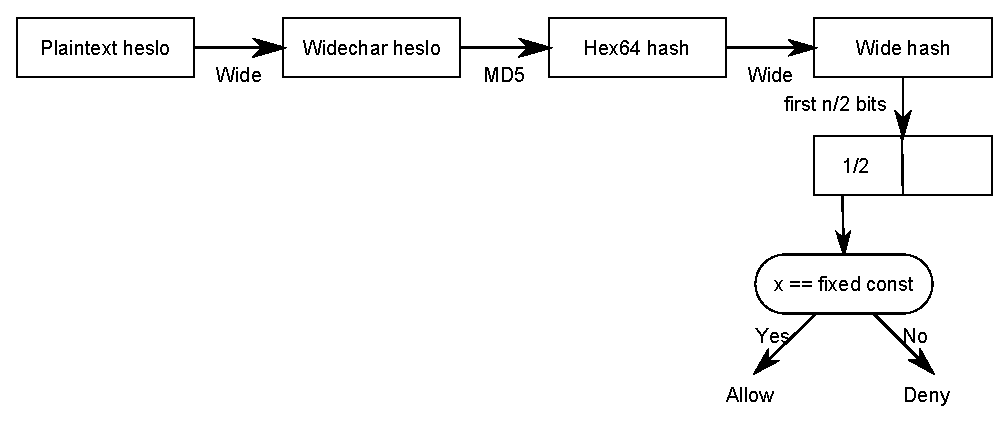
\includegraphics[scale=0.75]{img/0/extern_drive_encryption}
    \label{fig:extern_drive_encryption}
    \caption{Šifrovanie externého disku}
\end{figure}

Útok na tento systém je vcelku jednoduchý. Stačí v pamäti prepísať výsledok dešifrovacej transformácie. 

%Viac na:
%\url{http://www.h-online.com/security/news/item/NIST-certified-USB-Flash-drives-with-hardware-encryption-cracked-895308.html}

%A ešte na (pekny dokument nie priamo suvisiaci):
%Investigating 'secure'USB stickspsu.edu [PDF]
%PJ Bakker… - Citeseer
%\url{http://citeseerx.ist.psu.edu/viewdoc/download?doi=10.1.1.84.2539&rep=rep1&type=pdf}



\chapter{Krypto I}
\label{chapter:krypto}
\section{Interaktívne dokazovacie systémy}

V tejto časti sa budeme venovať dokazovacím systémom. Pôjde o akýsi
typ spoločného výpočtu dvoch účastníkov - jedného výpočtovo
neobmedzeného provera $P$ a výpočtovo obmedzeného overovateľa $V$.
Cieľom provera je akýmsi spôsobom presvedčiť overovateľa o znalosti
nejakého faktu.
Formálne,
interaktívnym dokazovacím systémom (IDS) nazveme dvojicu
$\langle P,V \rangle$, kde $P$ je pravdepodobnostný TS
s neobmedzenou výpočtovou silou,
$V$ je pravdepodobnostný TS pracujúci v polynomiálnom čase.
Oba stroje zdieľajú spoločný vstup $x$, môžu počas svojho výpočtu
komunikovať a o akceptovaní resp. zamietaní vstupu $x$ rozhoduje iba
$V$.
IDS pre jazyk $L$ je dvojica $\langle P,V \rangle$ pre ktorú platí
\begin{itemize}
\item {\bf úplnosť} -- $\forall x \in L:
    Pr[V\textit{ akceptuje } x \textit{ v systéme }
        \langle P,V \rangle ] \ge 2/3$
\item {\bf korektnosť} -- $\forall P^*: \forall x \not \in L:
    Pr[V\textit{ akceptuje } x \textit{ v systéme }
        \langle P^*,V \rangle ] \le 1/3$
\end{itemize}
Prvá podmienka hovorí o tom, že ak $x\in L$, dokazovateľ s veľkou
pravdepodobnosťou presvedčí overovateľa o správnosti.
Naopak, korektnosť tvrdí, že ľubovoľný (podvodný) dokazovateľ
presvedčí overovateľa na zlom vstupe len s nízkou pravdepodobnosťou.

\begin{poznamka}
    Pre $L \in P$ je jednoduché navrhnúť IDS. Overovateľ bude ignorovať
    komunikáciu a môže si vypočítať príslušnosť slova sám.
    Pre $L \in NP$ je jednoduché navrhnúť IDS posielajúci práve jednu
    správu -- konkrétny dôkaz, či výpočet NTS pre problém L.
\end{poznamka}

\begin{priklad}
    Uvažujme problém $GNI \not \in NP$ -- problém grafového neizomorfizmu.
    Vstup pozostáva zo zápisu dvoch grafov $G_0, G_1$, akceptovať chceme, keď
    dané dva grafy nie sú izomorfné. Môžeme použiť nasledovný protokol
    pri dôkaze: Uvažujme $k$ kôl, v každom z nich prebehne takáto
    komunikácia:
    %% FIXME: preco 'P \send V' je vizualne dlhsie ako 'V \send P'?
    \begin{itemize}
        \item $V$ si zvolí $i \inr \{0,1\}$ a permutáciu
         $\pi \inr perm(|G_i|)$
        \item $V \send P: H = \pi(G_i)$.
        \item $P \send V: i'$ reprezentujúce graf $G_{i'}$, s ktorým je $H$
        izomorfný ($P$ je neobedzene výpočtovo silný).
        \item $V$ zamietne vstup ak $i \not = i'$.
    \end{itemize}
    Po $k$ úspešných kolách $V$ akceptuje.

    Ak $G_0 \isomorph G_1$, tak $P$ má v každom kole šancu 50\% na
    uhádnutie indexu $i$, ktorý si vymyslí $V$. 
    Pravdepodobnosť akceptovania po $k$ kolách je teda $2^{-k}$.
    Naopak, ak $G_0 \not \isomorph G_1$, tak čestný dokazovateľ vie
    vždy odlíšiť permutáciu $G_0$ a $G_1$,
    čize akceptujeme s pravdepodobnosťou 1.
\end{priklad}

Pre interaktívne dokazovacie systémy sa dá dokázať mnoho zaujímavých
vlastností. Napríklad, že $IP=PSPACE$,
čiže inak povedané, čokoľvek čo
vieme robiť v polynomiálnom priestore vieme robiť interaktívnym
dokazovacím systémom. O tom, ako na to je písané napr. v
\cite{ip-pspace}. Aby sme neostali staromódni, nedávnym dôkazom
(August 2009) bolo $QIP=PSPACE$ \cite{qip-pspace}, čiže to,
že kvantové počítače nepomôžu sile interaktívnych dôkazov.
Dôkaz je veľmi technický a využíva viacero rôznych redukcií a známych
rovností tried zložitosti. Odporúčame si ho prečítať hlavne ak má
čitateľ pocit, že kvantovým výpočtom aspoň trochu chápe.

Ďalšou možnosťou, kam môžeme rozvíjať interaktívne dokazovacie systémy
sú takzvané MIP -- multiprover IP. Pri týchto akoby overovaťel mohol
krížovo vyslúchať dokazovateľov, ktorí so sebou nemôžu komunikovať.

\section{Zero knowledge}
Špeciálnym prípadom interaktívnych dokazovacích systémov sú takzvané
bezznalostné dôkazy. Základná myšlienka sa dá ilustrovať na príklade 
"Alibaba a jaskyňa tajomstiev".

Alibaba na svojich potulkách narazil (alebo skôr naďabil) na jaskyňu,
ktorá má čarovnú stenu. Táto stena sa na vyslovenie čarovnej formuly
otvorí a prepustí človeka na druhú stranu. Po dlhšom skúmaní
prišiel na to, že jaskyňa vyzerá ako na obr. \ref{fig:alibaba}. Pretože v
jaskyni neboli žiadne poklady (alebo boli, ale niekto ich stihol
vybrať skorej), Alibaba sa rozhodol zbohatnúť na TV show.
Bude ukazovať, že vie tajnú formulku a nafilmujú ho pritom. Nechce ale
prezradiť tajomstvo zvyšku sveta.

\begin{figure}[htp]
    \centering
    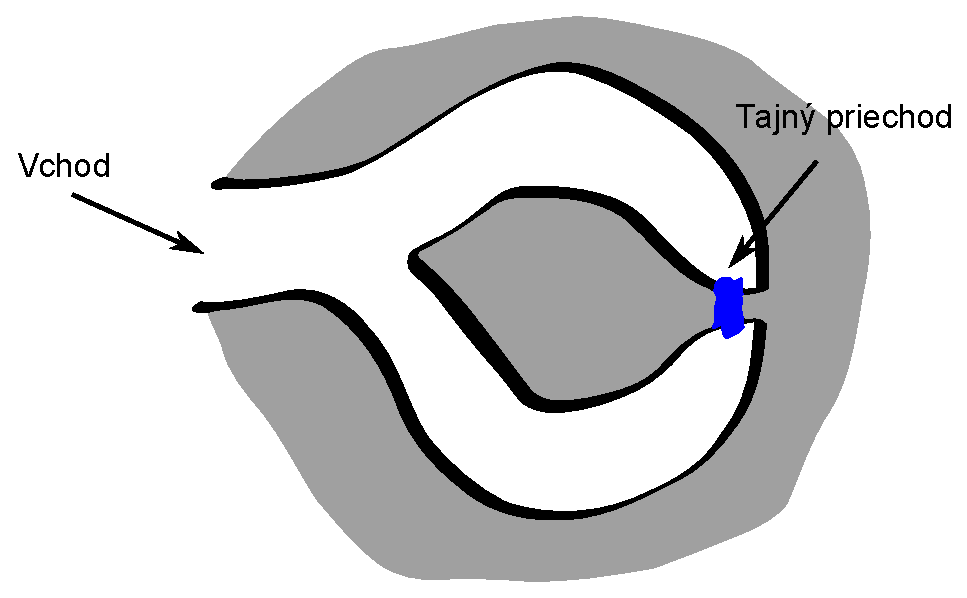
\includegraphics[scale=0.4]{img/x/alibaba}
    
    \label{fig:alibaba}
    \caption{Alibabova jaskyňa}
\end{figure}

Preto sa s filmármi dohodol na nasledujúcom postupe - vôjde do jaskyne
sám. Následne dnu vojde aj filmový štáb a ten zakričí Aladinovi, z
ktorej strany má dôjsť. Ten na demonštráciu znalosti prechádzania cez
steny vyjde zo správnej strany.

Poučenie z príbehu: Môžeme si všimnúť, že Aladin nikomu neprezradí
svoje tajomstvo. Zároveň ale presvedčí štáb o tom, že cez tie steny
chodí, pretože inak by si musel vedieť niekoľkokrát po sebe správne
tipnúť, čo sa mu rozhodnú zakričať, keď dôjdu na rázcestie.
Dôkaz má ale aj ďalšiu vlastnosť - Aladin síce presvedčil štáb, ale
môže presvedčiť aj divákov? Nie. Čo ak bolo napríklad video
"nastrihané" iba na dobré pokusy? Takémuto ``strihanie'' bude
vo formálnej definícii zodpovedať simulátor -- mohli by sme povedať,
že bude zastupovať šikovného strihača filmu, ktorý nepodarené pokusy
vystrihne.

Bezznalostné dokazovacie systémy sú preto také systémy, pri ktorých
dokazovateľ presvedčí overovateľa o svojej pravde bez toho aby mu
prezradil čokoľvek iné. Taktiež, ľubovoľný externý pozorovateľ
komunikácie nemá byť schopný odlíšiť reálny dôkaz od akéhosi
vykonštruovaného. 

\begin{definicia}[Zero knowledge]

Označme:
\begin{itemize}
\itemsep -1.2mm
    \item $V^*$ -- overovateľ (nečestný)
    \item $S^*$ -- simulátor, pravdepodobnostný stroj pracujúci
        v polynomiálnom čase
    \item $T(V^*, x)$ -- množina komunikácií na vstupe $x$
    \item $F(V^*, x)$ -- množina simulovaných komunikácií na vstupe $x$
    \item $p_t(x,y)$ -- pravdepodobnosť, že komunikácia na vstupe $x$
            bude $y$
    \item $p_f(x,y)$ -- pravdepodobnosť, že simulátor vygeneruje na
            vstupe $x$ komunikáciu $y$
\end{itemize}

Potom interaktívny dokazovací systém pre jazyk L je perfektné bezznalostný,
ak 
\begin{equation*}
    \forall V^*\ \exists S^*\ \forall x \in L \mbox{ platí }
        T(V^*, x) = F(V^*, x) \mbox{ a tiež } 
        \forall t \in T(V^*,x) \colon p_t(x,t) = p_f(x,t)
\end{equation*}

Teda ak simulátor vie generovať takú komunikáciu, ktorá má presne rovnaké rozloženie
pravdepodobnosti ako reálna komunikácia.
\end{definicia}

\begin{poznamka}
Pokiaľ sú distribúcie v množinách $T$ a $F$ nerozlíšiteľné
v polynomiálnom čase hovoríme, že systém je výpočtovo bezznalostný.
\end{poznamka}


\todo{zvysok, blackbox simulator}
\todo{ZK pre izomorfizmus}

\begin{poznamka}
    Na tomto mieste by sme upozornili čitateľa na fakt, že nami
    prezentovaný algoritmus v predchádzajúcej sekcii na neizomorfizmus grafov
    nie je bezznalostný.
    
    Prečo? Uvažujme falošného verifikátora $V'$,
    ktorý má graf $G$ a vie, že je izomorfný buď s $G_0$ alebo s
    $G_1$. V tomto prípade môže využiť provera $P$ ako orákulum na
    problém izomorfizmu grafov -- jednoducho mu pošle $G$, čo je
    validná správa a vráti sa mu index.

    No dobre. A ako súvisí to, že $V'$ vie niečo zistiť s definíciou
    bezznalosti, t.j. s existenciou simulátora? Jednoducho tak, že
    každý polynomiálny simulátor by musel vedieť simulovať komunikáciu
    $P$ s $V'$. Toto ale nemôže vedieť, pretože by sme vedeli v
    polynomiálnom čase riešiť izomorfizmus grafov, čo za predpokladu
    $P\neq NP$ nevieme. Preto dôkaz nie je bezznalostný z definície.
    Záverom teda môžeme usudzovať, že existencia polynomiálneho
    simulátora je naozaj ekvivalentná našej intuícii, čo to znamená
    "bezznalostný".

    Pre záujemcov o bezznalostný algoritmus pre neizomorfizmus grafov
    odporúčame prečítať \cite{nig}, kde je uvedené rozšírenie našeho
    postupu tak, aby $P$ nič neprezradil.
\end{poznamka}

\section{Bit commitment}

Bit commitment schéma je protokol pre dvoch účastníkov, kde sa najprv účastník
zaviaže k nejakému bitu (ktorý zatiaľ zostáva utajený pre ostatných) 
a následne po istom čase ho odhalí. Formálne to môžeme definovať takto:

\begin{definicia}
    Majme dve množiny $X,Y$ a funkciu $f\colon \{0,1\} \times X \mapsto Y$,
    ktorú vieme ``ľahko'' počítať.
    Od $f$ požadujeme navyše ešte tieto vlastnosti:
    \begin{itemize}
    \item \emph{vlastnosť utajenia} --
        Zo znalosti $f(b,x)$ je ťažké určiť $b$.

    \item \emph{vlastnosť záväznosti} --
        Je ťažké nájsť $x, y$ také, že $x \neq y$ a 
            $f(0,x) = f(1,y)$.
    \end{itemize}

    Potom bit commitment protokol vyzerá nasledovne:

    \begin{enumerate}
    \item $A$ si zvolí $b \in \{0,1\}$ ku ktorému sa chce zaviazať a
            taktiež si zvolí náhodný prvok $x \inr X$
    \item $A \to B$: $y = f(b,x)$ -- záväzok
    \item $A \to B$: $x$ -- odhalenie, môže prísť po istom čase
    \item $B$ overí, či $y = f(0,x)$ alebo $y = f(1,x)$
    \end{enumerate}
\end{definicia}

\noindent
Tento protokol môžeme realizovať viacerými spôsobmi:

\subsection{Bit commitment pomocou RSA}

Majme nejakú inštanciu RSA systému, teda trojicu $(n,e,d)$,
kde účastník $B$ nepozná súkromný kľúč.
Bit commitment realizujeme nasledovne:
\begin{enumerate}
    \item Záväzok: $A$ si zvolí $x \inr \mathbb{Z}_n^*$, také, že
        $b$ je najmenej významný bit $x$ a pošle 
        $y = x^e \pmod n$.
    \item Odhalenie: $A \send B:x$. Účastník $B$ overí, či
        $x^e \pmod n = y$.
\end{enumerate}

Vlastnosť utajenia je dodržaná, keďže možnosť zistiť $b$
je ekvivalentná rozbitiu RSA schémy.
Vlastnosť záväznosti je tiež dodržaná,
keďže k jednému $y$ existuje iba jedno $x$.
V tomto prípade ide o nepodmienenú bezpečnosť.

\begin{poznamka}
    V krypto I sme si spomínali, že posledný bit je v RSA bezpečný.
    Tak trochu sa tam ale zavádzalo. To, čo sa v skutočnosti dokázalo
    bolo totiž ``Ak vieme zisťovať posledný bit $\then$ vieme lámať
    RSA''. Otázka ale znie, čo ak vieme určovať posledný bit napr. s
    pravdepodobnosťou 51\% bez toho, aby to implikovalo zlomenie celej
    schémy? Odpoveď je, že nevieme, ako dokázali Chor a Goldreich v 
    \cite{rsa-lsb}.
\end{poznamka}

\subsection{Bit commitment pomocou diskrétneho logaritmu}
Majme konečnú grupu $G$ a jej prvky $g, h \in G$,
pričom v tejto grupe nevieme efektívne počítať diskrétny logaritmus.
Zároveň predpokladáme, že
nevieme diskrétny logaritmus $h$ pri základe $g$.
Realizácia funkcie $f(b,x)$ bude nasledovná: 
\begin{equation*}
    f(b,x) = g^x h^b
\end{equation*}

Utajenie je v tomto prípade nepodmienene bezpečné,
lebo existujú $x, y$ také, že: $g^x = g^y h$ 
a teda nevieme jednoznačne určiť $b$ zo znalosti $f(b,x)$.
Vlastnosť záväznosti výplýva z toho, že nepoznáme
diskrétny logaritmus $h$ pri základe $g$.

\todo{BC pomocou kvadratických rezíduí}

\subsubsection{Nepodmienená bezpečnosť a záväznosť}
Môžeme si všimnúť, že sme vedeli dosiahnúť pri jednej vlastnosti 
(utajenie, záväznosť) nepodmienenú bezpečnosť.
Nasledujúca veta hovorí o tom, že nepodmienenú bezpečnosť 
nevieme dosiahnúť pri oboch vlastnostiach.

\begin{veta}
Neexistuje bit commitment schéma, ktorá by garantovala 
nepodmienenú bezpečnosť pri utajení a záväznosti.
\end{veta}

\begin{dokaz}
Sporom. 
Uvažujeme funkciu bit commitment schémy $f(b,x)$.
Ak je táto schéma garantuje nepodmienenú záväznosť, tak
platí $\forall x, y\colon f(x,b_1) = f(y,b_2) \Rightarrow b_1 = b_2$
(teda neexistuje vhodná dvojica
$x, y$ ktorou by sme vedeli porušiť záväzok).
Z toho vyplýva, že keď dostaneme $z = f(x,b)$, tak vieme 
vyskúšaním všetkých možných hodnôt $(x,b)$ určiť vyhovujúce dvojice,
tieto ale musia mať rovnaký commitnutý bit.
Preto táto schéma nemôže garantovať nepodmienené utajenie.
\end{dokaz}
\todo{IDS pre ham cycle pomocou BC}



\section{Oblivious transfer}

Ďalším základným primitívom, na ktorom vieme budovat kryptografické
prvky je takzvaný oblivious transfer. Ide o akýsi prenos údajov,
pričom sender sa nedozvie, či boli údaje prenesené, prípadne ktoré
údaje boli prenesené.

\begin{definicia}[1-2 OT]
    1-2 oblivious transferom nazveme komunikáciu podľa nasledujúcej
    schémy:
    \begin{itemize}
        \item $A \send B: m_0, m_1$, kde $m_0$ a $m_1$ sú 2 rôzne
        správy, ktoré chce $A$ poslať.
        \item $B$ si vyberie niektorú zo správ, ktorú chce prijať a
        toto prijatie mu bude umožnené.
        \item $A$ sa nedozvie, ktorú správu $B$ prijal.
        \item $B$ nemá možnosť prijať obe správy naraz.        
    \end{itemize}
\end{definicia}

\begin{definicia}[50\% OT]
    50\% oblivious transferom nazveme komunikáciu podľa nasledujúcej
    schémy:
    \begin{itemize}
        \item $A \send B: m$, kde $m$ je správa.
        \item $B$ s spravdepodobnosťou 50\% správu prijme, inak sa o
        nej nedozvie nič.
        \item $A$ sa nedozvie, či $B$ správu prijal
    \end{itemize}
\end{definicia}

\begin{priklad}[Realizácia 50\% OT]
    Nech $A$ chce poslať správu účastníkovi $B$ s 50\%-nou
    pravdepodobnosťou úspechu. Na začiatku si $A$ zvolí inštanciu RSA
    s $n=pq$, kde $p,q$ sú veľké prvočísla. Bude nasledovať
    komunikácia
 \begin{itemize}
    \compactlist
    \item $A \send B: n,e,E(m)$ 
    \item $B$ si zvolí $x \inr Z_n$
    \item $B \send A: x^2$
    \item $A$ s pomocou faktorizácie vyberie nejakú odmocninu
        $z \inr \{x,-x,y,-y\}$.
    \item $A \send B: z$.
    $B$ vie faktorizovať $n$ (a dešifrovať správu) s
    pravdepodobnosťou 50\% (ak $z \not = \pm x$, tak jednoducho
    spočíta pomocou $\nsd(z-x, n)$).
 \end{itemize} 
\end{priklad}

\begin{priklad}[Realizácia 1-2 OT]
 1-2 OT budeme realizovať za pomoci diskrétneho logaritmu.
 Účastník $A$ si zvolí grupu $G$, $n=|G|$ a generátor $g\in G$.
 \begin{itemize}
    \compactlist
    \item $A \send B: c \inr G$.
    \item $B$ si zvolí $b\in\{0,1\}$ - číslo správy, ktorú chce
    prijať.
    \item $B$ si zvolí $x \inr G$ a vypočíta hodnoty $y_b = g^x$,
    $y_{1-b} = c/ y_b$. Platí $y_0 y_1 = c$ a tiež existuje (pretože
    $g$ je generátor) hodnota $x': g^{x'} = y_{1-b}$. Teda, $A$ nevie
    odlíšiť jednotlivé hodnoty.
    \item $B \send A: y_0$.
    \item $A$ si zvolí $k_0,k_1 \inr G$ a vytvorí šifrované správy 
    $E_0 = \langle g^{k_0}, y_0^{k_0} \xor m_0 \rangle$,
    $E_1 = \langle g^{k_1}, y_1^{k_1} \xor m_1 \rangle$.
    \item $A \send B: E_0, E_1$.
    \item $B$ dešifruje $m_b$ ako $(g^{k_b})^x \xor (y_b ^ {k_b} \xor
    m_b)$.
    Pokiaľ $B$ nevie riešiť DH problém, druhú správu nedostane.
    \todo{dokaz}
 \end{itemize}
\end{priklad}

\subsection{Konverzie}

\begin{lema}
    50\% OT sa dá simulovať pomocou 1-2 OT.
\end{lema}
\begin{dokaz}
    Postup je jednoduchý. Nech $A$ chce poslať správu 
    $m \ne 0$.\footnote{Predpokladáme, že vieme posielať správy, ktoré
        sú dlhšie ako 1 bit.\fixme{ako spravit konveziu z 1 bitu?}
    }
    Nech $c \inr \{0,1\}$ a nech $m_c = m, m_{1-c} = 0$. $A$ pošle
    správy $m_0, m_1$ pomocou 1-2 OT. $B$ prijme správu $m$ s
    pravdepodobnosťou 50\%, inak prijme 0 a vie, že sa prenos
    nepodaril.
\end{dokaz}

\todo{1-2 OT pomocou 50}
\todo{BC pomocou 50 OT}
Pre záujemcov je predchádzajúca konštrukcia presnejšie popísaná v
\cite{ot_equiv}.

\section{Bezpečný výpočet viacerých účastníkov}

Uvažujme nasledujúci problém ``starých dám''. Dve dámy sa stretnú a
chceli by zistiť, ktorá z nich je staršia.\footnote{V skutočnosti
sa každá chce ubezpečiť, že tá druhá je staršia :-)}
Neboli by to však dámy v svojom veku, kebyže o sebe nechcú nič prezradiť.
Presnejšie povedané -- nechcú prezradiť nič iné okrem informácie, ktorá z
nich je staršia. Navyše budeme predpokladať, že dámy budú
spolupracovať a jedna druhú nepodrazí.
Teraz navrhneme protokol, ktorý túto ich dilemu vyrieši.

Uvažujme, že vek môže nadobúdať len jednu z konečne veľa diskrétnych
hodnôť (napríklad $v_A,v_B \in V = \{1,\dots,100\}$).
Ďalej uvažujme inštanciu asymetrického šifrovacieho systému s
veľkosťou šifrovacieho kľúča $N$. 
Budeme požadovať, aby účastník $A$ vedel (efektívne) iba šifrovať.

\begin{itemize}
    \compactlist
    \item $A$ si zvolí $x$ -- náhodné $N$-bitové číslo.
        Pomocou tohoto čísla budeme ``maskovať''  $v_A$.
    \item $A \send B: c = E(x) - v_A $ (pošleme maskované $v_A$).
    \item $B$ vygeneruje čísla $y_1, \dots, y_{100}$ tak aby
            $y_i = D(c + i)$ (kde $y_{v_A} =x$, ostatné hodnoty
            sú nepredikovateľné).
    \item $B$ si teraz vygeneruje náhodné $N/2$ bitové prvočíslo $p$ a
    vypočíta $z_1,\dots,z_{100}$ ako $z_i = y_i \pmod{p}$.
    Ak by náhodou existovali indexy $i,j: |z_i - z_j| < 2$, tak si
    zvolí iné prvočíslo.
    \item $B \send A:p$ a 100 čísel $t_1, \dots, t_{100}$ --
        budú to hodnoty $z_i$ zvýšené o hodnotu predikátu
        $v_B < i$, teda hodnoty
        $z_1,\ z_2,\ \dots,\ z_{v_B}, \
         z_{v_B+1}+1,\ z_{v_B+2}+1,\ \dots,\ z_{100}+1$.
    \item $A$ sa teraz pozrie na pravdivosť
        $x \pmod{p} \overset{?}{=} t_{v_A}$. Ak tvrdenie platí,
        tak $v_A \le v_B$.
    \item $A \send B:$ výsledok porovnania
\end{itemize}
Je jasné, že $B$ nemá šancu sa dozvedieť nič o hodnote $v_A$ počas
výpočtu, pretože $A$ si mohol zvoliť $x$ pre ľubovoľnú hodnotu
$v_A$ ako $x=D(c + v_A)$ s rovnakou pravdepodobnosťou.\footnote{V
    skutočnosti musí kryptografický systém spĺňať nejaké požiadavky
    navyše, aby to platilo, čitateľ si môže premyslieť aké.
}
Otázne teda je, či $A$ sa môže dozvedieť niečo o $v_B$.
Na to by ale potreboval vedieť dešifrovať hodnoty $y_i$, čo sme
zamietli v predpokladoch.
\begin{poznamka}
    Samozrejme, náš dôkaz ``správnosti'' by ostražitého čitateľa nemal
    presvedčiť úplne. V takomto prípade je odporúčané nazrieť do
    \cite{yao}.
\end{poznamka}

\todo{bezpecny vypocet funkcie}



\chapter{Krypto II}
\label{chapter:krypto2}
\section{Absolútne bezpečná šifra}

Tento krát sa ideme zaoberať nepodmienenou bezpečnosťou. Uvažujme 
výpočtovo neobmedzene silného útočníka a cypher text only attack (COA).
Požadujeme aby útočník zo znalosti šifrového textu nezískal nič nové.

Označme množinu otvorených textov ako $P$, kľúčov ako $K$, šifrových textov ako $C$
(uvažujeme iba množinu reálne možných šifrových textov). Každému $x \in P$ vieme priradiť
pravdepodobnosť výskytu $pr(x)$, pravdepodobnosť
výskytu konkrétneho kľúča $k \in K$ označíme ako $pr(k)$. Predpokladáme, že
konkrétny kľúc používame iba raz a že jeho voľba nezávisí od otvoreného textu.
Takisto pravdepodobnosť výskytu šifrového textu $c \in C$ označíme $pr(c)$. Táto pravdepodobnosť
bude vždy väčšia ako nula (keďže uvažujeme len šifrové texty, ktoré môžu vzniknúť zašifrovaním).
Všetky tieto množiny považujeme za konečné.

\begin{definicia}
    Šifrovací systém $(E,D)$ je absolútne bezpečný ak:
    $$\forall x \in P, \forall c \in C\colon pr(x | c) = pr(x)$$
\end{definicia}
\begin{komentar}
    Táto definícia vlastne hovorí o tom, že znalosť šifrového textu útočníkovi nepovie nič
    nové, keďže distribúciu pravdepodobnosti otvorených textov pozná.
\end{komentar}

Niekoľko zaujímavých vlastností:
Vzhľadom na to, že dešifrovanie musí byť uskutočniteľné, musí platiť $|C| \geq |P|$.
Ďalej určite platí $|K| \geq |P|$, ináč by sme pri znalosti šifrového textu mohli 
vyskúšať dešifrovanie všetkými kľúčmi a niektoré otvorené texty by sme mohli vylúčiť
($pr(x|c) = 0$). Zaujímavá je situácia keď $|P| = |C| = |K|$, tú popisuje nasledujúca veta:

\begin{veta}{(Shanon)}
    Nech $(E,D)$ je šifrovací systém, kde $|P|=|C|=|K|$. Potom tento šifrovací systém je
    absolútne bezpečný práve vtedy, keď sú splnené nasledujúce vlastnosti:
    \begin{enumerate}
        \item $\forall k \in K\colon pr(k) = \frac{1}{|K|}$
        \item $\forall x \in P, \forall y \in C: \exists! k \in K\colon E_k(x) = y$
    \end{enumerate}
\end{veta}

\begin{dokaz}
    \noindent
    \begin{itemize}
    \item[$\Rightarrow:$] 
        Nech systém $(E,D)$ je absolútne bezpečný.
        Ak by pre $x \in P, y \in C$ neexistoval kľúč $k \in K$ taký, 
        že $E_k(x) = y$, útočník zo znalosti $y$ vie vylúčiť otvorený text $x$,
        čo odporuje tomu, že systém $(E,D)$ je absolútne bezpečný. 
        Keďže $|C|=|K|$, tak tento kľúč môže byť maximálne jeden 
        (keby ich bolo viac, tak by $\exists z \in C$ taký, že
        $x$ nevieme zašifrovať na $z$). 

        Keďže $P$ je konečná, môžeme otvorené texty očíslovať, 
        teda $P = \{ x_1, x_2, \dots, x_n\}$. 
        Teraz fixujme $c \in C$. Pre každý otvorený text musí platiť:
        \begin{equation*}
            pr(x_i) = pr(x_i | c) = \frac{pr(c | x_i) pr(x_i)}{pr(c)}
        \end{equation*}
        a teda
        \begin{equation*}
            pr(c) = pr(c | x_i) = pr(k_i)
        \end{equation*}
        kde $k_i \in K$ je taký kľúč, že platí $E_{k_i}(x_i)=c$. 
        Z toho vyplýva, že všetky kľúče majú rovnakú pravdepodobnosť a keďže
        súčet výskytu ich pravdepodobnosti je $1$, tak 
        $\forall k \in K\colon pr(k) = \frac{1}{|K|}$.

    \item [$\Leftarrow:$]
        Vypočítame $pr(x|c)$ a ukážeme, že definícia platí. Vieme, že:
        \begin{equation*}
            pr(x|c) = \frac{pr(c|x)pr(x)}{pr(c)}
        \end{equation*}
        Ďalej $pr(c|x) = pr(k)$, kde $E_k(x)=c$ a teda 
        $pr(c|x) = \frac{1}{|K|}$. Ešte treba určiť $p(c)$.
        \begin{equation*}
            pr(c) = \sum_{k \in K} pr(k) pr(D_k(c)) = 
                \frac{1}{|K|} \sum_{x \in P} pr(x) = \frac{1}{|K|}
        \end{equation*}
        (Pri dešifrovaní všetkými možnými kľúčmi dostaneme 
        všetky možné otvorené texty (a každý práve raz). 
        A súčet pravdepodobností výskytu všetkých otvorených textov je 1).

        Takže dostávame:
        \begin{equation*}
            pr(x|c) = \frac{pr(c|x)pr(x)}{pr(c)} = 
                \frac{\frac{1}{|K|} pr(x)}{\frac{1}{|K|}} = pr(x)
        \end{equation*}

        A teda systém $(E,D)$ je absolútne bezpečný, čím je náš dôkaz hotový.
    \end{itemize}
\end{dokaz}

\begin{priklad}
    Vernamova šifra je príklad absolútne bezpečného šifrovacieho systému.
\end{priklad}

Iným uhlom pohľadu na absolútne bezpečnú šifru je nerozlíšiteľnosť 2 otvorených textov. 
Teda útočník dostane dva otvorené texty a jeden šifrový text a má určiť, z ktorého otvoreného
textu šifrový text vznikol. Tu nesmie uspieť.

\begin{veta}
    Šifrovací systém $(E,D)$ je absolútne bezpečný práve vtedy, keď:
    \begin{equation*}
        \forall x_1 \in P, \forall x_2 \in P, \forall c \in C
            \colon pr(c|x_1)=pr(c|x_2)
    \end{equation*}
\end{veta}

\begin{dokaz}
    \noindent
    \begin{itemize}
    \item[$\Rightarrow:$] 
        Vieme, že $pr(c|x_1) = \frac{pr(x_1|c) pr(c)}{pr(x_1)}$. 
        Keďže systém $(E,D)$ je absolútne bezpečný, 
        tak $pr(x_1|c) = pr(x_1)$, čiže $pr(c|x_1) = p(c)$. 
        To isté dostaneme aj pre $x_2$.

    \item[$\Leftarrow:$]
        $pr(c|x)$ je rovnaká pre všetky $x \in P$, čiže je konštantná. 
        Nech $pr(c|x) = t$. Potom
        \begin{equation*}
            pr(c) = \sum_{k \in K} pr(k) pr(c|D_k(c)) = 
                t \sum_{k \in K} pr(k) = t
        \end{equation*}
        Čiže $pr(x|c) = pr(x)$, čo sme chceli dokázať.
    \end{itemize}
\end{dokaz}

Takto môžeme podať trochu inú definíciu absolútne bezpečnej šifry.

\begin{definicia}
    Uvažujme kryptoanalytickú hru s nasledovným priebehom:
    \begin{enumerate}
        \item Útočník $A$ pošle druhej strane $B$ dva otvorené texty $p_1, p_2$.
        \item $B$ si zvolí náhodne $b \inr \{0,1\}$
            a náhodný kľúč $k \in K$.
        \item $B\send A: c = E_k(p_b)$.
        \item $A$ sa snaží zistiť z ktorého otvoreného textu $c$ vznikol. 
            Svoj úsudok pošle ako $b'$.
        \item Ak $b' = b$, tak $A$ uspel. V opačnom prípade neuspel.
    \end{enumerate}
    Pokiaľ je systém $(E,D)$ absolútne bezpečný, 
    tak pravdepodobnosť úspechu $A$ je $\frac{1}{2}$.
\end{definicia}

Dá sa ukázať, že tieto dve definície sú ekvivalentné.
\todo{dokaz}

\subsection{PSS -- Probabilistic signature scheme}

PSS je dokázateľne bezpečná (za istých predpokladov) schéma na
digitálne podpisy. Navrhli ju páni Mihir Bellare a Philip Rogaway
v \cite{pss}. Celá schéma je vlastne akýmsi znáhodnením hashovania -- k
správe sa pridá náhodný reťazec dĺžky $k_0$ a hash sa počíta až
potom. Samozrejme, pri overovaní hashu treba nejakým spôsobom
vyriešiť, aby sme sa dozvedeli použitý náhodný reťazec. Ako sa ukáže
neskôr, toto nie je až taký veľký problém ak použijeme ďalšiu
hashovaciu funkciu.

PSS má oproti doteraz spomínaným schémam jednu veľkú výhodu -- pri
dôkaze jej bezpečnosti sa ukáže ``tesná'' hranica. T.j., možnosť
prelomiť PSS s pravdepodobnosťou $\eps$ priamo umožňuje lámanie RSA s
rovnakou pravdepodobnosťou.


\subsubsection{RSA-PSS}

Podpisová schéma $PSS[k_0,k_1]=\langle GenPSS,SignPSS,VerifyPSS\rangle$ je
parametrizovaná dvoma hodnotami $k_0, k_1$.
Generovanie kľúča $k$ je presne rovnaké ako v $GenRSA\mbox{-}FDH$.

Pri podpisovaní bude náš algoritmus používať dve hashovacie funkcie.
Prvú si označíme $h$ a nazveme ju kompresor, pretože bude skracovat
správu, $h:\{0,1\}^* \rightarrow \{0,1\}^{k_1}$.
Druhá funkcia bude $g$ (nazvaná aj generátor), pričom
$g:\{0,1\}^{k_1} \rightarrow \{0,1\}^{k-k_1-1}$.

Ešte si označíme $g_1$, resp. $g_2$ ako funkciu, ktorá vracia
prvých $k_0$ (resp. zvyšných $k-k_0-k_1-1$) bitov funkcie $g$.

Na obrázku \todo{} je schematicky naznačený postup podpisovania
podľa pseudokódu \ref{proc:signpss}

% {{{ proc SignPSS
\begin{procedure}
    \caption{SignPSS($m$)}
    \label{proc:signpss}
    $r \inr \{0,1\}^{k_0}$\;
    $w \assign h(M \concat r)$\;
    $r^* \assign g_1(w) \xor r$\;
    $y \assign 0 \concat w \concat r^* \concat g_2(w)$\;
    \Return $y^d \bmod N$\;
\end{procedure}
%% }}}

Môžeme si všimnúť, že náhodný reťazec $r$ sme neuviedli v
``otvorenom'' tvare, ale zviazali sme ho funkciou $g_1$. Intuitívne,
toto nám umožní zaručiť jeho integritu a zároveň máme možnosť ho
zrekonštruovať.

Overovanie podpisu je popísané v pseudokóde \ref{proc:verifypss}

%%% {{{ proc VerifyPSS
\begin{procedure}
    \caption{VerifyPSS($m$,$x$)}
    \label{proc:verifypss}
    $y \assign x^e \bmod N$\;
    rozdeľ $y$ na $b \concat w \concat r^* \concat \gamma$\;
    $r \assign r^* \xor g_1(w)$\;
    \eIf{$(b \ne 0) \vee (g_2(w) \ne \gamma) 
            \vee (h(m \concat r) \ne w)$}
    {% then
        \Return reject\;
    }{% else
        \Return accept\;
    }
\end{procedure}
%%% }}}

\todo{nejake omacky okolo funkcnosti a preco je  to zhruba tak
spravene}

\subsubsection{Dôkaz bezpečnosti}
\todo{dokaz bezpecnosti - tesna redukcia}

\section{Faktorizácia}

\subsection{Náhodné zobrazenia}
Ešte predtým, ako sa vrhneme na algoritmy pre faktorizáciu, zhrnieme
si niekoľko užitočných tvrdení, ktoré budeme neskôr využívať. Jedná sa
hlavne o vlastnosti náhodného zobrazenia.

Majme náhodné zobrazenie $f:X \rightarrow X$, kde $|X| = n$.
Budeme uvažovať postupnosť $x_0 = s,\ x_1=f(s)=f(x_0),\ x_2 =
f(f(s))=f(x_1),\ \dots,\ x_{i+1} = f(x_{i})$ pre nejaké začiatočné $s$.
Keďže obor hodnôt je konečný, najviac po $n$ krokoch sa nám nejaké
číslo zopakuje a dostaneme cyklus. Vo všeobecnosti môžeme postupnosť
rozdeliť na začiatočný ``chvost'' dĺžky $\lambda$ a cyklus dĺžky
$\mu$, ako na obrázku \ref{fig:cyclelen}.

\begin{figure}[h!]
    \centering
    \includegraphics[scale=0.9]{img/03/cyclelen.1.mps}
    \caption{Chvost a telo cyklu pri náhodnom zobrazení}
    \label{fig:cyclelen}
\end{figure}

\noindent
Základom pre ďalšiu analýzu bude nasledujúce tvrdenie:

\begin{lema}
    Nech $f:X\rightarrow X, |X|=n$ je náhodné zobrazenie.
    Potom pre $n\rightarrow \infty$ platí
    $\lambda \sim \sqrt{\pi n/8}$ a 
    $\mu \sim \sqrt{\pi n/8}$.
\end{lema}
\begin{dokaz}
    Dôkaz nebudeme robiť, nakoľko vyžaduje netriviálne znalosti
    z generujúcich funkcií. Čitateľ ho môže nájsť napríklad v článku
    \cite{randommap}.
\end{dokaz}

Za pomoci predchádzajúceho tvrdenia môžeme hľadať ``kolízie'' v
postupnosti v očakávanom čase $\Theta(\sqrt{n})$.
Jednoduchým riešením je napríklad použiť hashovanie na každý prvok
postupnosti $x_i$. Praktický problém, ku ktorému ale narážame je
pamäť, ktorá by musela byť $\Theta(\sqrt{n})$, čo je v dnešnej dobe
limitujúci faktor. Existujú však aj metódy na hľadanie cyklov,
ktoré používajú konštantnú pamäť.

\subsubsection{Metódy na hľadanie cyklov}

Začneme Floydovou metódou, ktorá sa niekedy aj označuje metódou dvoch
bežcov. Pracuje na veľmi jednoduchom princípe -- predstavme si, že máme
2 bežce -- ukazovatele na prvky postupnosti. Ak jedným bežcom budeme
pohybovať rýchlejšie ako druhým a oba tieto prvky ležia v cykle, po
istom čase (najneskôr celý prechod cyklu) jeden z ukazovateľov dobehne
ten prvý. Formálne, metóda porovnáva nasledujúce dvojice prvkov:
$(x_1,x_2),\ (x_2,x_4),\ (x_3,x_6),\ (x_4,x_8),\ \dots$.
Jej funkčnosť dokážeme nasledovne: Predpokladajme, že v aktuálnom
kroku algoritmu máme prvky $x_i, x_{j=2i}$. Ďalej redpokladajme,
že oba tieto prvky ležia v cykle, ktorého dĺžka je $\lambda$.
Ak by platilo $i \equiv j \pmod{\lambda}$, tak nutne platí $x_i = x_j$.
Uvažujme teda, že rovnosť nenastáva. V tom prípade ale platí 
$j-i \equiv i \pmod{\lambda}$. Na začiatku je táto hodnota 0 
a každým krokom algoritmu vzrastie o 1. Čiže,
najneskôr o $\lambda$ krokov bude $j-i \equiv 0 \pmod{\lambda}$.
Preto môžeme časovú zložitosť algoritmu ohraničiť ako $O(\mu+\lambda)$.

\begin{algorithm}
    \caption{Floydov algoritmus na hľadanie cyklov}
    \label{algo:floyd}
    $x1 \assign f(s)$\;
    $x2 \assign f(f(s))$\;
    \While{$x1 \ne x2$}{
        $x1 \assign f(x1)$\;
        $x2 \assign f(f(x2))$\;
    }
    output $\assign$ prvok cyklu je $x1$\;
\end{algorithm}

\medskip
Ďalšou metódou je Brentova metóda detekcie cyklov. Má rovnakú
asymptotickú časovú zložitosť ako Floydova, v praxi však používa menej
výpočtov funkcie $f$ a preto je zväčša preferovaná.
Metóda funguje v akýchsi blokoch mocniny dvojky.
Porovnáva hodnotu $x_{2^i}$ postupne s nasledujúcimi číslami
$x_{2^i+k}$, až dosiahneme ďalšiu mocninu dvojky, vtedy začneme ďalším
blokom. Algoritmus skončí v okamihu, keď je dĺžka aktuálneho bloku
(mocnina dvojky) väčšia ako dĺžka cyklu a už sme do cyklu vošli.
Preto je čas Brentovej metódy $O(\lambda + \mu)$.
Graficky je to naznačené na obrázku \ref{fig:brent} a príslušný
algoritmus je \ref{algo:brent}.

\begin{figure}[h!]
    \centering
    \includegraphics{img/03/brent.1.mps}
    \caption{Brentova metóda na hľadanie cyklov}
    \label{fig:brent}
\end{figure}

\begin{algorithm}
    \caption{Brentov algoritmus}
    \label{algo:brent}
    $x1 \assign f(s)$\;
    $x2 \assign f(f(s))$\;
    $i \assign 2$\;
    \While{$x1 \ne x2$}{
        \If{$i$ je 2. mocnina}{
            $x1 \assign x2$\;
        }
        $x2 \assign f(x2)$\;
        $i \assign i+1$\;
    }
    output $\assign$ prvok cyklu je $x1$\;
\end{algorithm}

\subsection{Pollardova metóda na faktorizáciu}
\todo{Pollard}
\todo{Dixon}
\todo{Quadratic sieve}

\section{Algoritmy na výpočet diskrétneho logaritmu}
Počas celej tejto kapitoly sa budeme pohybovať v cyglickej grupe 
$G, |G|=n$ generovanej generátorom $g \in G$.
Našim cieľom bude vypočítať diskrétny logaritmus prvku $y$
pri základe $g$, t.j. nájsť hodnotu $x$, takú, že $g^x=y$ (počítané
v grupe $G$).


Triviálnym algoritmom je postupné skúšanie možných hodnôt $x$, teda
$g^0,g^1,\dots,g^{n-1}$.
Časová zložitosť je v tomto prípade $O(n)$, pamäťová $O(1)$.

\subsection{Shanksov Baby-step/giant-step algoritmus}
Baby-step/giant step je spôsob, ako preliať čas do pamäte.
Algoritmus sa skadá z 2 častí - ``veĺkých'' a ``malých'' krokov.
Veľké kroky sa dajú predpočítať raz, malé kroky treba robiť pre každé
číslo, z ktorého chceme zistiť diskrétny logaritmus.

Najskôr budeme robiť "veľké kroky".
Zoberme si $t=\lfloor \sqrt{n} \rfloor$.
Vypočítajme si postupne hodnoty $g^0,g^t,\dots,g^{\lfloor n/t \rfloor t}$.
Pre každú hodnotu, ktorú takto vypočítame si zapamätáme (napríklad do
hashovacej tabuľky) aj jej diskrétny logaritmus, t.j. zapamätáme si hodnoty
$(k,g^{kt})$ pre $k=0,1,\dots,\lfloor n/t \rfloor t$.
Táto časť algoritmu trvá $O(t)$, teda $O(\sqrt{n})$, potrebná pamäť je
tiež $O(t)=O(\sqrt{n})$.

Po tomtp predpočítaní môžeme pokračovať malými krokmi.
Počítajme postupne hodnoty $y g^0,yg,yg^2,\dots, yg^{t-1}$ a pozeráme sa,
či niektorá z týchto hodnôt sa nenachádza v zapamätanej tabuľke.
Grafické znázornenie činnosti celého algoritmu je na obrázku
\ref{fig:babygiant}.
\begin{figure}[h]
    \centering
    \includegraphics{img/04/babygiant.1.mps}
    \label{fig:babygiant}
    \caption{Kroky v baby-step/giant-step algoritme}
\end{figure}

Zložitosť druhého kroku je maximálne $t$ krát tabuľkový lookup, pretože
najneskôr o $t$ hodnôt narazíme na nejakú hodnotu, ktorá už v tabuľke bude.
Dokopy teda po oboch krokoch nájdeme diskrétny logaritmus
v čase $O(\sqrt{n})$ a pamäti $O(\sqrt{n})$.

Problém pamäťovej zložitosti sa snaží riešiť Pollardov algoritmus.

\subsection{Pollardov $\rho$ algoritmus}
Podobne ako pri faktorizácii sa budeme snažiť nájsť nejakú funkciu, ktorá
by sa správala ako čo najlepšie náhodné zobrazenie. Pri takejto funkcii
potom môžeme očakávať nájdenie cyklu/kolízie v čase $O(\sqrt{n})$.

Zvoľme si $x_0 = g^{a_0} y^{b_0}$ kde $a_0,b_0 \inr Z_{n-1}$.
$x_0$ bude začiatočný prvok postupnosti. Na ``znáhodnenie'' našej funkcie
si grupu $G$ rozdelíme na 3 disjunktné množiny:
$G=S_1 \union S_2 \union  S_3$.

Potom môžeme uvažovať nasledujúcu funkciu $f$:
\begin{equation*}
    x_{i+1} = f(x_i) =
        \begin{cases}
         y x_i & x_i \in S_1 \\
         x_i^2 & x_i \in S_2 \\
         g x_i & x_i \in S_3
        \end{cases}
\end{equation*}
Je dôležité, že vďaka operáciam, ktoré sme zvolili, vieme vypočítať aj
"rozklad" $x_{i+1}$ nasledovne:

\begin{equation*}
    (a_{i+1},b_{i+1}) =
        \begin{cases}
         (a_i,b_i+1) & x_i \in S_1 \\
         (2a_i,2b_i) & x_i \in S_2 \\
         (a_i+1,b_i) & x_i \in S_3 \\
        \end{cases}
\end{equation*}

Našim cieľom je teda nejak rozdeliť $G$ na $S_1,S_2,S_3$ tak, aby
funkcia $f$ čo najviac pripomínala náhodné zobrazenie.
Pre prvočíselné grupy to môžeme napríklad rozdeliť modulo 3.
Pre všeobecné grupy môže byť dobrý spôsob zobrať hash vnútornej binárnej
reprezentácie prvku a tento hash zobrať modulo 3.

Keď už máme funkciu $f$ danú, môžeme použiť niektorý z algoritmov na
hľadanie cyklov spomínaných v kapitole o faktorizácii.

Ak nájdeme kolíziu, dostávame
\begin{align*}
    g^{a_i} y^{b_i} &= g^{a_j} y^{b_j} \\
    y^{b_i-b_j} &= g^{a_j-a_i} \\
    x &=(a_j - a_i)(b_i-b_j)^{-1} \pmod n
\end{align*}
a teda vieme $x$ vypočítať.

Časová zložitosť algoritmu (ak predpokladáme,
že $f$ má charakteristiku náhodného zobrazenia) je
$O(\sqrt{n})$, pamäťová zložitosť $O(1)$.

\subsection{Pohligov-Hellmanov algoritmus}
Tento algoritmus funguje vo všeobecnosti, ale veľmi efektívny je hlavne v
prípade, že $n$ má prvočíselný rozklad s malými prvočíslami.
$n=p_1^{m_1} \dots p_k^{n_k}$
\todo{dokoncit algoritmus}



\subsection{Index calculus}
Narozdiel od predchádzajúcich algoritmov, tento algoritmus nie je
všeobecný. Dá sa použiť napríklad $(Z_p^*,\cdot), GF(2^m)$.
V prípade eliptických kriviek sa nedá použiť. Tento jeho hendikep
ale kompenzuje jeho časová zložitosť, ktorá je subexponenciálna.

Uvažujme pre jednoduchosť grupu $G=(Z_p^*,\cdot)$.
Algoritmus pozostáva z 2 krokov - predvýpočtu a samotného výpočtu.
Predvýpočet sa môže spraviť raz pre jednu grupu.

Predvýpočet:

Majme zvolenú prvočíselnú bázu $B=\{p_1,\dots,p_b\}$.
Položme $a \inr Z_{p-1}$. 
Našou snahou bude rozložiť $g^a$ nad bázou $B$, teda nájsť hodnoty
$e_1,\dots,e_b$ také, že $g^a \mod p = p_1^{e_1} p_2^{e_2} \dots
p_b^{e_b}$.
Našou ambíciou je nazbierať čo najviac takýchto závislostí, optimálne
$b+1$. Ak totiž zlogaritmujeme dané rovnosti, dostaneme sústavu
lineárnych rovníc.
$a=e_1 \dlog_g p_1 + e_2 \dlog_g p_2 + \dots + e_b \dlog_g p_b \pmod{p-1}$.
V tejto sústave sú neznáme $\dlog_g p_1, \dlog_g p_2, \dots, \dlog_g p_b$.

Ak sme úspešne zvládly tento predvýpočet, môžeme skúšať počítať dlog y
nasledovne.
Zvolíme si $b\inr Z_{p-1}$ a skúšame, či vieme hodnotu
$y g^a = p_1 ^ {e_1} \dots p_b ^ {e_b}$. Tým pádom
$x+a = e_1 d_1 + \dots + e_b d_b$.

Časová zložitosť (veľmi podobná Dixonovmu algoritmu) je
$O(e^{(1+O(1))\sqrt{\log p \log \log p}})$.

\begin{poznamka}
    Výpočet v prípade, že $G$ je $GF(p^m)$ je veľmi podobný, bázu budú ale
    tvoriť ireducibilné polynómy.
\end{poznamka}
\begin{poznamka}
    Nech G je podgrupa $Z_p^*$, ktorej veľkost $|G|=q$ je prvočíslo.
    Ak mame generator $g\in G$, potom výpočet $\dlog_g x$ v $G$ 
    realizujeme buď pollard rho metodou.
    \todo{doplnit}
\end{poznamka}

\section{Bezpečnosť niektorých hašovacích funkcíí}

S hašovacími funkciami sme sa zoznámili v zimnom semestri.
Pripomeňme, že je to zobrazenie $h: X \to Y$, kde $Y$ je konečná množina.
Pre jednoduchosť predpokladajme, že $Y = \{0,1\}^n$. 

Dobrá hašovacia funkcia by mala spĺňať nasledovné požiadavky 
(vychádzajú z toho, že by sa mala čo najviac priblížiť náhodnému orákulu). 
Okrem požiadaviek zo zimného semestra formulujeme niekoľko ďalších:
\begin{enumerate}
\itemsep -1.2mm
\item Odolnosť prvého vzoru: K danému $y$ je ťažké nájsť $x$ také, 
že $h(x) = y$. Očakávaný čas hľadania $x$ je $\Theta(2^n)$.
\item Odolnosť druhého vzoru: K danému $x$ je ťažké nájsť 
$z \neq x$ také, že $h(x) = h(z)$. Očakávaný čas hľadania je opäť
$\Theta(2^n)$.
\item Odolnosť proti kolíziám: Je ťažké nájsť $x \neq x$ také, 
že $h(x) = h(z)$. Očakávaný čas hľadania je $\Theta(2^{n/2})$ (narodeninový útok).
\vskip 0.5cm
\item $k$-odolnosť prvého vzoru: K danému $y$ je ťažké nájsť navzájom rôzne 
$x_1, x_2, \dots, x_k$ také, že $h(x_i) = y$. Očakávaný čas hľadania
je $\Theta(k 2^n)$.
\item $k$-odolnosť druhého vzoru: K danému $x$ je ťažké nájsť navzájom rôzne 
$x_1, x_2, \dots, x_k$ také, že $h(x_i) = h(x)$ a $x_i \neq x$.
Očakávaný čas hľadania je $\Theta(k 2^n)$.
\item $k$-odolnosť proti kolíziám: Je ťažké nájsť navzájom rôzne 
$x_1, x_2, \dots, x_k$ také, že $\forall i, j\colon h(x_i) = h(x_j)$. 
Dá sa ukázať, že pokiaľ je $k$ zanedbateľné oproti $2^n$, tak očakávaný 
čas hľadania $k$-kolizie je $\Theta(2^{\frac{n(k-1)}{k}})$.
Pre väčšie $k$ je očakávaný čas väčší.
\end{enumerate}

\subsection {Iteratívne konštrukcie hašovacích funcíí a ich slabiny}

Rozdeľme text $M$ na rovnakodlhé bloky $m_1, m_2, \dots, m_l$
(v poslednom bloku môžeme očakávať nejaký padding).
Položme $h_0 = IV$ a $h_i = f(h_{i-1}, m_i)$ pre $i \geq 1$, kde $f$ 
je kompresná funkcia, ktorej obor hodnôt je $\{0,1\}^n$.
Výstupom hašovacej funkcie je hodnota $h_l$. Takúto konštrukciu 
používa väčšina v súčasnosti používaných hašovacích funkcií
(MD5, SHA-1, SHA-xxx, \dots).

\begin{figure}[h!]
    \label{fig:iter}
    \centering
    \includegraphics[scale=1.0]{img/05/iter.1.mps}
    \caption{Iteratívna hašovacia funkcia}
\end{figure}


V roku 2004 \cite{Joux04} bol nájdený nasledovný útok:
\begin{enumerate}
\itemsep -1.2mm
\item Položme $h_0 = IV$.
\item Nájdime $m_1 \neq m_1'$ také, že $f(h_0, m_1) = f(h_0, m_1') = h_1$, 
toto vieme v čase $O(2^{n/2})$.
\item Podobne nájdime dvojice $m_2 \neq m_2', \dots, m_k \neq m_k'$ také, 
že $f(h_{i-1}, m_i) = f(h_{i-1}, m_i') = h_i$.
\item Toto celé vieme spraviť v čase $O(k 2^{n/2})$. A dostaneme $2^k$ 
kolidujúcich textov (pre každý z $k$ blokov si môžeme vybrať
2 rôzne texty). Hash každého z nich bude $h_k$.
\end{enumerate}

\begin{figure}[h!]
    \label{fig:joux1}
    \centering
    \includegraphics[scale=1.0]{img/05/joux.1.mps}
    \caption{Útok na multikolíziu}
\end{figure}


Samotný tento útok ešte veľa neznamená. Ale ukazuje sa, že
ho vieme využiť na nájdenie podstatnejších slabín.

Ukážeme si rýchlejšie hľadanie $2^k$-vzoru:
\begin{enumerate}
\itemsep -1.2mm
\item Nájdeme $2^k$-kolíziu.
\item Následne nájdeme posledný blok $m_{k+1}$ tak, aby $f(h_k, m_{k+1}) = y$. Toto vieme v čase $O(2^n)$.
\end{enumerate}

\begin{figure}[h!]
    \label{fig:joux2}
    \centering
    \includegraphics[scale=1.0]{img/05/joux.2.mps}
    \caption{Využitie multikolízie pri hľadaní multivzoru}
\end{figure}

Celkový čas hľadania bude $O(2^n)$ namiesto očakávaného $\Theta(k 2^n)$. Presne rovnako vieme hľadať aj druhý vzor.

Niekedy v záujme zvýšenia bezpečnosti niekedy zreťazujeme za sebou výstup dvoch rôznych hašovacích funkcíí, napr.
MD5 a SHA-1. Dostaneme takzvanú kaskádovú hašovaciu funkciu, formálne $H(m) = H_1(m)||H_2(m)$. 
Ukazuje sa, že ak v jednej z týchto dvoch hašovacích funkcíí vieme efektívne hľadať multikolízie, tak vieme
v kaskádovej hašovacej funkcii hľadať kolízie efektívnejšie ako len narodeninovým útokom.
Pre jednoduchosť predpokladajme, že obor hodnôt $H_1$
a $H_2$ je $\{0,1\}^n$. Teda dĺžka výstupu $H$ je $2n$ a teda očakávaný čas hľadania kolízie je $\Theta(2^n)$.
Predpokladajme, že $H_1$ je iteratívna. Potom vieme v čase $O(\frac{n}{2} 2^{n/2})$ nájsť $2^{n/2}$ kolízií. Tieto dosadíme
na vstup $H_2$ a narodeninový paradox nám zaručí vysokú úspešnosť nájdenia kolízie aj pre $H_2$. Takto sme dostali
kolíziu pre $H$ v čase $O(n 2^{n/2})$.

\subsection{Hľadanie expandovateľnej správy a jej využitie}

Niekedy je výhodné mať kolidujúce správy rôznej dĺžky. 
V nasledujúcom texte si popíšeme nájdenie takej multikolízie,
kde všetky správy majú rôzne dĺžky. Nech $m^*$ je ľubovoľný
text dĺžky 1 blok.
Označme ako $F(h_i, a_1||a_2||\dots||a_x) = f(f(\dots f(h_i, a_1), a_2), \dots, a_x)$,
teda viackrát za sebou použitú kompresnú funkciu $f$.
Postup je podobný ako pri hľadaní multikolízie:
\begin{enumerate}
\itemsep -1.2mm
\item Položme $h_0 = IV$
\item Nájdime $m_1$ a $m_1'$ také, že: $f(h_0, m_1) = f(f(h_0, m^*), m_1') = F(h_0, m^*||m_1') = h_1$. 
\item Nájdeme ďalšie dvojice $m_2, m_2', \dots, m_k, m_k'$ také, že platí:
$f(h_{i-1}, m_i) = F(h_{i-1}, (m^*)^{2^{i-1}}||m_i') = h_i$
\item Každú dvojicu vieme nájsť v čase $O(2^{n/2})$. Celkový čas bude $O(k 2^{n/2})$.
Dostali sme opäť $2^k$ rôznych kolidujúcich textov, ktoré tentokrát 
majú dlžky $k, k+1, \dots, k+2^k-1$ blokov. 
Blok príslušnej dĺžky nájdeme tak, že od dĺžky odpočítame $k$, následne
sa pozrieme na binárny zápis výsledku postupne odzadu. Ak je tam $0$, ideme
po hrana, ktorá nemá $m^*$, v prípade $1$ ideme po tej druhej.
\end{enumerate}

\begin{figure}[h!]
    \centering
    \includegraphics{img/05/expand.1.mps}
    \caption{Konštrukcia multikolízie rôznej dĺžky}
    \label{fig:expand1}
\end{figure}


Pri niektorých hašovacích funkciách, ktoré využívajú
Davies-Meyerovu konštrukciu vieme expandovateľnú správu hľadať
ešte jednoduchšie. Príkladom môže byť SHA-1, ktorej kompresná funkcia
je definovaná nasledovne:
$f(h, m) = E_m(h)+h$

Zoberme náhodné $m$. Potom vieme vypočítať tzv. pevný bod, teda vnútorný
stav ktorý sa po \clqq zhašovaní\crqq $m$ nezmení:
$$f(h,m) = h$$
$$E_m(h) + h= h$$
$$h = E_m^{-1}(0)$$

Vypočítajme si $2^{n/2}$ pevných bodov $h_1, h_2, \dots, h_{2^{n/2}}$ a k ním príslušné správy
$m_1, m_2, \dots, m_{2^{n/2}}$. 
Následne skúšajme rôzne $m'$ a hľadajme také, kde $f(h_0, m') = h_i$, kde $i \in \{1, 2, \dots 2^{n/2}\}$.
Vďaka narodeninovému paradoxu stačí $2^{n/2}$ pokusov. Takto sme v čase $O(2^{n/2})$ našli správu, ktorú
vieme ľubovoľne natiahnuť.
\todo{OBRAZOK}

Následne hľadanie expandovateľnej správy vieme využiť na efektívnejšie hľadanie druhého vzoru ako hrubou silou.
Majme správu, ktorá je dlhá $k + 2^k - 1$ blokov. Následne zostrojme expandovateľnú správu dĺžky $k$, ktorej hash je $h_k'$.
Následne skúšajme nájsť  $\tilde{m}$ také, že $f(h_k', \tilde{m})$ sa rovná niektorej z hodnôt $h_{k+1}, \dots h_{k+2^k-1}$. Ak áno 
(označme takú hodnotu ako $h_x$), tak môžeme bloky $m_1, m_2, \dots, m_x$ nahradiť príslušnou expandovateľnou správou.
Očakávaný počet pokusov je $\Theta(2^{n-k})$. 

Čo to v praxi znamená? Zoberme bežne používanú SHA-1, ktorej výstup má 160 bitov. Teda,
očákavaný počet operácií pre nájdenie druhého vzoru je úmerný $2^{160}$. Maximálna dĺžka správy
pre SHA-1 je $2^{64} - 1$ bytov, čo je asi $2^{55}$ blokov. Zoberme správu dĺžky
$54 + 2^{54} - 1$ blokov. Najprv v čase $2^{80}$ nájdeme expandovateľnú správu (SHA-1 je DM konštrukcia).
Následne potrebujeme ešte $2^{106}$ pokusov na nájdenie \clqq spájacieho\crqq bloku.
Toto je síce stály veľký počet, ale oproti očakávanému počtu je to značné zlepšenie.

\subsection{Obrana pred týmto druhom útokov}
Tieto útoky ukazujú, že iteratívna konštrukcia nie je najvhodnejšia.
To, čo ju môže zachrániť je mať aspoň 2-krát dlhší medzistav 
(t.j. hodnoty $h_1, h_2, \dots, h_{k-1}$). Potom sa skomplikuje hľadanie
kolízií v medzistavoch a konštrukcia je proti týmto útokom bezpečná.

\subsection{Nostradamov útok}

Uvažujme nasledujúcu situáciu. Svetovo známy prorok Nostradamus
vyriekne začiatkom roka 2009 proroctvo, týkajúce sa budúcnosti.
Môže to byť napríklad stav akciového indexu na konci roka 2010.
Akurát ho nezverejní (nechce predsa ovplyvniť burzu) a zverejní
len hash tohoto proroctva (v podstate je to niečo ako commitment).

Následne na konci roka odhalí svoje proroctvo. Hash je v poriadku, proroctvo
o akciách hovorí pravdu, za ním sú ešte nejaké ďalšie proroctvá.
Otázkou je ako veľmi môžeme veriť tomu, že prorok poznal stav
akcií na konci roka. Ukazuje sa, že na iteratívnu konštrukciu
hašovacích funkciu existuje tzv. chosen prefix attack.

\subsubsection{Konštrukcia ``proroctva''}

Pripravme si najprv $2^k$ hodnôt $h_{0,1}, h_{0,2}, \dots, h_{0,2^k}$.
Následne hľadajme $m_{0,1}, m_{0,2}, \dots, m_{0,2^k}$ také, že
\begin{align*}
    f(h_{0,1}, m_{0,1}) &= f(h_{0,2}, m_{0,2}) = h_{1,1} \\
  &  \dots \\
    f(h_{0,2^k-1}, m_{0,2^k-1}) &= f(h_{0,2^k}, m_{0,2^k}) = h_{1,
        2^{k-1}} 
\end{align*}
Následne pokračujme podobným spôsobom aj na ďalších úrovniach
pokiaľ nedostaneme jedinú hodnotu $h_{k,1}$.
Túto hodnotu zverejníme ako hash nášho proroctva.
Navyše, aby sme za správu vedeli \clqq prilepiť\crqq rozumný obsah,
je vhodné aby tieto správy dávali aspoň nejaký zmysel.

Aký čas strávime prípravou tohoto stromu?
Nájdenie jednej kolízie trvá čas $O(2^{n/2})$, na prvej úrovni treba 
$2^{k-1}$ kolízii, na druhej $2^{k-2}$ a na poslednej
potrebujeme jednu kolíziu. Celkový čas je teda
$O(2^n (2^{k-1} + 2^{k-2} + \dots + 1)) = O(2^{n/2} 2^k)$.
Lepší spôsob je nehľadať kolízie na jednotlivých úrovniach po dvojiciach,
ale rovno pre celú úroveň.
Vtedy na prvej úrovni strávime čas $O(2^{k/2 + n/2})$. 
Celkový čas bude tiež $O(2^{k/2 + n/2})$.

\begin{figure}[h]
    \centering
    \includegraphics[scale=0.9]{img/05/nostradamus.1.mps}
\end{figure}

Nostradamus na konci roka (po zatvorení burzy) zistí stav akciového
trhu a pripraví si podľa neho správu.
Označme ju $m$. Po jej zahashovaní sa dostaneme do odtlačku
$h_m$. Teraz hľadáme správu $\tilde{m}$, pre ktorú platí
$f(h_m, \tilde{m}) = h_{0,x_0}$, kde $x_0 \in \{1, 2, \dots, 2^k\}$.
Následne na základe pripraveného stromu vieme za správu dolepiť patričné 
$m_{0,x_0}, m_{1,x_1}, \dots, m_{k,x_k}$ také, že
výsledný hash bude predtým zverejnený $h_{k,1}$.
\fixme{jazykove okienko - ten hash alebo ta hash?}
Teda na konci zverejníme správu 
$m || \tilde{m} || m_{0,x_0} || m_{1,x_1} || \dots || m_{k, x_k}$.

Čas hľadania $\tilde{m}$ bude $2^{n-k}$.

\subsubsection{Celkový čas útoku}
Bolo by dobré, aby čas trvania oboch častí útoku bol viacmenej vyvážený. 
Uvažujme najprv pomalšiu variantu predspracovania.
Vtedy chceme, aby $2^{n-k} = 2^{k+n/2}$, z čoho dostaneme
$k=\frac{n}{4}$ a celkový čas bude $2^{\frac{3}{4} n}$.
Pri rýchlejšom predspracovaní máme podmienku $2^{n-k} = 2^{k/2 + n/2}$,
z čoho máme $k = \frac{n}{3}$ a celkový čas $2^{\frac{2}{3}n}$.

\fixme{realne priklady}

\section{Jednorázové a fail-stop podpisové schémy}

Jednorázové podpisové schémy, ako už ich názov napovedá, slúžia na
podpísanie práve jednej správy. Ich bezpečnosť je v prípade viacnásobného
podpisovania ohrozená. Načo sú nám teda takéto podpisové schémy? Zatiaľ to
vyzerá tak, že sú iba menej výhodné. Existujú však dôvody, prečo sa zaoberať
aj takýmito zjavne ``okrátenými'' podpisovými schémami.

Ich hlavná výhoda bude spočívať v jednoduchších predpokladoch pri dôkaze
bezpečnosti. Kým pri bežných podpisových schémach sme stavali na
tažkosti istých matematických problémov (RSA, dlog, Diffie-Hellman),
pri jednorázových schémach nám bude stačiť napríklad jednosmernosť
hashovacej funkcie.\footnote{Už aj toto je pomerne náročný predpoklad,
    keďže nevieme povedať veľa o existencii one-way funkcií}
Druhou výhodou môže byť rýchlosť -- zrejme je jednoduchšie hashovať hodnoty
ako napríklad umocňovať.
Treťou výhodou (i keď skôr teoretickou) je možnosť odolať kvantovým
výpočtom -- pre väčsinu používaných ťažkých problémov sú známe kvantové
algoritmy, ktoré ich efektívne počítajú. Pre invertovanie hashovacích
funkcií ale takéto algoritmy nie sú známe.

Otázka teda môže znieť, že či jednorázovosť je až taká obmedzujúca
vlastnosť. Môžeme napríklad uvažovať komunikáciu s bankou a podpisovanie
prevodných príkazov. Je jednoducho predstaviteľné, že
bežný človek za mesiac nespraví viac ako povedzme 20 príkazov.
Preto môžeme použiť
niečo ako pohľad z opačnej strany -- namiesto toho, aby sme navrhovali
podpisové schémy na polynomiálny počet podpísaných správ,
môžeme sa snažiť navrhnúť schémy na jednorázové podpisy a tie potom
rozšíriť nejakým spôsobom pre viac správ.

Jednorázovú podpisovou schému formálne definujeme veľmi podobne ako bežné
podpisové schémy

\begin{definicia}[Jednorázová podpisová schéma]
    je trojica algoritmov 
    $\langle Gen, Sign_{sk}, Verify_{pk} \rangle$ kde
    $Gen(1^k) \rightarrow \langle pk, sk \rangle$ je generátor kľúčov,
    $Sign_{sk}(m) \rightarrow \sigma$ je podpisovací algoritmus a
    $Verify_{pk}(m,\sigma) \rightarrow \{0,1\}$ je overovací algoritmus.
\end{definicia}

Pojem bezpečnosti takejto schémy si upravíme na jednu správu.
\begin{definicia}[Bezpečnosť]
    Uvažujme útočníka ako PPT algoritmus, ktorý má navyše k dispozícii
    orákulum $Sig_{sk}$. Útočník sa môže raz opýtať orákula na podpis
    $\sigma$ správy $m$ a jeho cieľom je zostrojiť
    správu $m' \ne m$ a k nej platný podpis $\sigma'$.
    Budeme hovoriť, že schéma je bezpečná ak pravdepodobnosť,
    že ľubovoľný útočník uspeje (t.j. nájde $(m',\sigma')$), je zanedbateľná.
\end{definicia}

\subsection{Lamportova schéma}

Uvažujme, že máme funkciu $f: X \rightarrow Y$, ktorá je jednosmerná.
Budeme podpisovať správy $m$ fixnej veľkosti $|m|=n$. Toto samo o sebe nie
je žiadny problém, ak uvážime, že budeme podpisovať len hash správy, ktorý je
fixnej veľkosti.

Generovanie kľúča bude vyzerať nasledovne:

%%% {{{ proc GenLamport
\begin{procedure}[H]
    \caption{GenLamport($n$)}
    \For{$i:=1$ \KwTo $n$}{
        $x_{i,0} \inr X$\;
        $x_{i,1} \inr X$\;
        $y_{i,0} \assign f(x_{i,0})$\;
        $y_{i,1} \assign f(x_{i,1})$\;
    }
    \Return $\langle sk=(x_{1,0},x_{1,1},\ldots,x_{n,0},x_{n,1}),\quad
             pk=(y_{1,0},y_{1,1},\ldots,y_{n,0},y_{n,1}) \rangle$\;
\end{procedure}
%%% }}}

Čitateľ už môže tušiť, ako budeme podpisovať správu -- jednoducho postupne
podpíšeme všetky jej bity tým, že zverejníme príslušnú časť súkromného
kľúča.

%%% {{{ SignLamport
\begin{procedure}[H]
    \caption{SignLamport($m$)}
    \For{$i:=1$ \KwTo $n$}{
        $\sigma_i \assign f(x_{i, m_i})$\;
    }
    \Return $\sigma = (\sigma_1, \ldots, \sigma_n)$
\end{procedure}
%%% }}}

Overovanie spočíva v overení každého podpísaného bitu správy.

%%% {{{ VerifyLamport
\begin{procedure}[H]
    \caption{VerifyLamport($m, \sigma$)}
    \For{$i:=1$ \KwTo $n$}{
        \If{$f(x_{i, m_i}) \ne y_{i, m_i}$}{
            \Return reject\;
        }
    }
    \Return accept\;
\end{procedure}
%%% }}}

Bezpečnosť schémy je založená na nasledujúcom pozorovaní:
Aby bol útočník k správe $m$ a jej podpisu $\sigma$ vygenerovať
falošnú správu $m' \ne m$ a jej podpis $\sigma'$, musel by byť schopný
vygenerovať $x_{i,b}$ pre nejakú novú dvojicu $(i,b)$.
To ale znamená invertovať niektorú hodnotu $y_{i,b}$ z verejnej
funkcie a to predpokladáme, že je možné iba so zanedbateľnou
pravdepodobnosťou.

Na druhej strane, schéma je evidentne jednorázová.
Až na špeciálny prípad, keď sú podpísané dve správy $m_1,m_2$ líšiace
sa v práve jednom bite (vtedy si útočník nepomôže), vieme kombinovať
jednotlivé bity podpisov a podpísať inú správu. V prípade, že
podpisujeme hash hodnotu, je navyše očakávané, že správy sa budú líšiť
na zhruba polovici bitov.

\medskip
Uvažujme teraz praktické aspekty používania takejto schémy. Podpisujme
hash, napríklad výstup z funkcie SHA-256. Ďalej predpokladajme, že
$|X|=|Y|=256 \unit{bit}$. Potom dostávame pre súkromný kľúč veľkosť
$|sk|=2*256*256 \unit{bit} =16 \unit{kB}$. Verejný kľúč je rovnako dlhý, čiže
$|pk|=16 \unit{kB}$ a podpis má polovičnú dĺžku kľúčov - $|\sigma|=8
\unit{kB}$.
V porovnaní napríklad s RSA je to výrazne horšie. Bolo by teda dobré
nejakým spôsobom skrátiť kľúče.

\subsubsection{Skrátenie súkromného kľúča}

Namiesto celého kľúča $(x_{1,0}, x_{1,1},
\ldots x_{n,1})$ si budeme pamätať iba náhodné $x \inr X$ -- seed pre
pseudonáhodý generátor, ktorý postupne vygeneruje dané hodnoty
$x_{i,b}$. Problém v tomto prípade je ďalší predpoklad -- bezpečnost
pseudonáhodného generátora (t.j. že z niektorých hodnôt postupnosti
$x_{1,0}, \ldots, x_{n,1}$ nevieme efektívne vypočítať žiadnu ďalšiu -
to by bolo ekvivalentné zlomeniu podpisovej schémy).

\subsubsection{Skrátenie verejného kľúča}
Namiesto celého kľúča zverejníme iba hash
$y=H(y_{1,0},y_{1,1},\ldots,y_{n,1})$. Tým pádom ale pri podpisovaní
musíme uviesť aj všetky hodnoty $y$, aby si to overovateľ mohol
overiť. Po chvíli zamyslenia sa ale môžeme pozorovať, že na overenie
stačí poslať tie hodnoty $y_{i,b}$, ktoré si overovateľ nemôže
spočítať. Tieto sú presne negácie bitov správy a teda nám stačí poslať
iba polovicu hodnôt $y_{i,b}$. Podpis sa nám tým predĺži na $16
\unit{kB}$.

\subsubsection{Merkleho konštrukcia}
Ďalši nezávislú možnosť ako skrátiť dĺžku postupnosti vymyslel
Merkle. Hlavnou pointou bude pridať akúsi formu checksumu -- počtu
nulových bitov správy. Potom budeme pri podpisovaní podpisovať iba
jednotkové bity, čím ušetríme v priemernom prípade takmer polovicu bitov
(čiže v našom prípade $|\sigma| \approx 4 \unit{kB}$).

Presnejšie, majme správu dĺžky $l$. K nej pridáme checksum dĺžky
$\lceil \log l \rceil$ a na výsledok dĺžky $n=l+\lceil \log l \rceil$
použijeme podpis, kde podpíšeme iba jednotkové bity.

V prvom rade by sme mali ukázať, že takáto zmena nepokazí bezpečnosť
schémy. Majme preto známu správu $m$ s podpisom $\sigma$ a
predpokladajme, že sa útočník snaží vyrobiť $m'$.
Ak existuje bit $i$, $m_i=0$ a platilo by $m'_i=1$, tak sa dostávame
do známej situácie, kedy útočník musí vyrobiť platný vzor pre $y_{i,1}$.
Ošemetná situácia ale nastáva, ak máme bit $m_i=1$ a útočník ho zmení
na nulu. V tomto prípade totiž nemusí nič podvrhnúť, lebo pre nulový
bit nemusí nič uviesť. Zachráni nás však checksum -- totiž, ak zmenšíme
celkový počet jednotiek v správe (a to jediné nám ostáva, ak nemáme
nablyšťanú guľu na lámanie one-way funkcie), vznikne nám aspoň jedna
jednotka na doteraz neodhalenom mieste. Nie je totiž možné, aby sme
po pričítaní čísla k checksume dostali checksumu pozostávajúci iba zo
známych bitov -- to by znamenalo, že daná checksuma používa iba
niektoré jednotky z pôvodnej, lenže to je v spore s tým, že je
väčšia. Preto aj v tomto prípade musí útočník úspešne nájsť vzor
jednosmernej fukncie a schéma ostáva naďalej bezpečná.

Ďalšou príjemnou vlastnosťou tejto úpravy je automatické zmenšenie
súkromného a verejného kľúča na polovicu - vôbec nepotrebujeme
generovať $x_{i,0}$ a $y_{i,0}$.

\subsection{Merkleho stromy}

Ako sme už písali, jedna z možností ako ``vylepšiť'' našu schému
je nájsť spôsob, ako z jednorazovej schémy spraviť schému na pár
použití. Jednoduchý spôsob je vygenerovať potrebný počet inštancií
schémy a zverejniť príslušné verejné kľúče. Problém tohoto prístupu je
čisto praktický -- musíme zverejniť veľmi dlhý verejný kľúč (všetky
verejné kľúče). V prípade, že máme napríklad jednu centrálnu autoritu,
ktorá vydáva súkromné kľúče a na svojej stránke zverejňuje všetky
verejné kľúče, môže to robiť isté problémy.

Preto by sme chceli akýmsi spôsobom zredukovať údaje o všetkých
verejných kľúčoch do nejakého odtlačku. Môžeme to spraviť rekurzvívne
-- označme si $H_{i,j}$ ako odtlačok všetkých kľúčov v intervale $<i,j>$.
Potom môžeme definovať rekurzívne $H_{l,r}=h(H_{l,m} || H_{m+1,r})$ kde
$m$ je stred medzi $l$ a $r$, čiže $m=\lfloor (l+r)/2 \rfloor$ a
$h$ je hashovacia funkcia. Takýmto spôsobom môžeme vybudovať celý
strom.
\begin{figure}[h]
    \centering
    \includegraphics{img/06/merkle.1.mps}
    \caption{Merkleho strom}
    \label{fig:merkle}
\end{figure}

Použitie bude nasledovné: Ako verejný kľúč zverejníme $H_{1,n}$. Toto je
malá hodnota a preto sa dobre distribuuje. Následne, predpokladajme, že
chceme použiť na podpisovanie kľúč číslo $x$. Na to, aby sme mohli overiť
podpis potrebujeme vedieť overiť celú cestu od kľúča $x$ ku koreňu. Toto
môžeme spraviť nasledovne -- zverejníme hodnotu pre každého súrodenca
nejakého vrcholu na ceste (týchto súrodencov si označíme ako
``autentifikačnú cestu'').
Ak totiž vieme vypočítať hodnotu vrchola na ceste a poznáme
súrodenca, tak vieme vypočítať hodnotu otca daného vrcholu.
Teda ak vieme hodnotu $pk_x$ a poznáme hodnoty všetkých súrodencov po ceste ku
koreňu, vieme postupne vypočítať hodnotu až ku koreňu. Následne stačí
overiť, či vypočítaná hodnota sedí so zverejnenou hodnotou $H_{1,n}$.

\begin{figure}[h]
    \centering
    \includegraphics{img/06/merkle.2.mps}
    \caption{Autentizačná cesta pre kľúč č.4}
    \label{fig:merkle}
\end{figure}

Pri tomto riešení teda pri jednom podpise musíme zverejniť popri podpise aj
celú autentiazačnú cestu, jej dĺžka je logaritmická od počtu kľúčov, ktoré
chceme používať. Je teda len na nás, či obetujeme zväčšenie podpisu na to,
aby sme mohli mať menší verejný kľúč.

Ďalšia zaujímavá otázka je výpočet autentifikačnej cesty. Vo všeobecnosti
pri veľkom strome totiž vypočítať jednotlivé potrebné hodnoty môže trvať až
čas úmerný počtu kľúčov. Toto sa dá riešiť na úkor pamäte udržiavaným istej
predpočítanej množiny vrcholov. Druhá možnosť je, ak chceme používať kľúče
zaradom v podarí $1,2,\dots,n$, existujú isté algoritmy na iteratívne
počítanie, kedy z autentifikačnej cesty pre kľúč $k$ vypočítame cestu pre
kľúč $k+1$ v amortizovanom čase $O(\log n)$, dokonca sa dá vynechať aj
amortizovanosť, ako sa píše v \cite{merkle_iter}.

Viac o Merkleho stromoch a iných vylepšeniach Lamportovej schémy
možno nájsť v \cite{merkle}.

\subsection{Stanekova schéma}
\todo{}

\subsection{Fail/stop podpisové schémy}

Predstavme si, že chceme schému pri ktorej sme (ako podpisovateľ) chránený pred neobmedzene výpočtovo silným
falšovateľom. Inak povedané, žiadny útočník, nech je akokoľvek silný,
by nemal z prístupu k môjmu verejnému kľúču byť schopný generovať
platné podpisy. Toto je samozrejme mierne v rozpore s tým, že máme
vedieť overiť podpis. Preto budeme požadovať miernejšiu vec -
podpisovateľ bude schopný preukázať, že to nebolo podpísané jeho
súkromným kľúčom.
Opäť si predstavíme jednorázovú schému. Útočník v prípade získania
správy, jej podpisu a verejného kľúča nebude schopný identifikovať
jednoznačne súkromný kľúč (napríklad preto, že možných súkromných
kľúčov bude veľmi veľa)
a nebude schopný vyrobiť správny podpis inej správy.
Pokiaľ sa falšovateľ pokúsi podpisať inú správu, tak podpisovateľ zistí, že bol použitý iný
ako jeho súkromný kľúč a je to schopný preukázať.

\subsubsection{Heyst Pedersenova schéma}

Uvažujme grupu $G$, kde $|G| = q$ a $q$ je nejaké (dostatočne veľké) prvočíslo.
Zoberme generátory $g, h \in G$.
Súkromný kľúč bude štvorica  $sk = (x_1, x_2, y_1, y_2) \inr Z_q$.
Poznamenajme, že narozdiel od ElGamalovej schémy, hodnoty $x,y$ sú
náhodné a \emph{nezávislé}.
Verejný kľúč bude dvojica
$pk = (g^{x_1} h^{x_2}, g^{y_1} h^{y_2}) = (z_1, z_2)$, teda akýmsi
spôsobom previažeme obe hodnoty. Algoritmický zápis generovania je vo
funkcii \ref{funct:genhp}

\begin{function}[h!]
    \caption{GenHP($G$)}
    \label{funct:genhp}
    $g,h \assign $ rôzne generátory $G$\;
    $x_1,x_2,y_1,y_2 \inr G$\;
    $z_1 \assign g^{x_1} h^{x_2}$\;
    $z_2 \assign g^{y_1} h^{y_2}$\;
    \Return $sk=(g,h,x_1,x_2,y_1,y_2), pk=(g,h,z_1,z_2)$\;
\end{function}

Správu $m$ podpíšeme svojim súkromným kľúčom ako lineárnu kombináciu
$x_i, y_i, m$ pomocou funkcie \ref{funct:signhp}
\begin{function}[h!]
    \caption{SignHP($m$)}
    \label{funct:signhp}
    $\sigma_1 \assign x_1 + m y_1$\;
    $\sigma_2 \assign x_2 + m y_2$\;
    \Return $\sigma=(\sigma_1,\sigma_2)$\;
\end{function}

Overenie podpisu je jednoduché otestovanie
rovnosti:
\begin{function}[h!]
    \caption{VerifyHP($\sigma,m$)}
    \eIf{$g^{\sigma_1} h^{\sigma_2} == z_1 z_2^m$}{
        \Return accept\;
    }{
        \Return reject\;
    }
\end{function}

Teraz si dokážeme niekoľko vlastností tejto schémy.

\begin{lema}
Pre ľubovoľnú trojicu $pk, m, \sigma$, kde $\sigma = SigHP_{sk}(m)$
a $sk$ je nejaký vyhovujúci súkromný kľúč
existuje $q$ rôznych kľúčov $sk^*$, takých že $\sigma = Sig_{sk^*}(m)$.
\end{lema}

\begin{dokaz}
Nech $h = g^a$, $z_1 = g^{e_1}$ a $z_2 = g^{e_2}$ 
(neobmedzene silný útočník vie $a, e_1, e_2$ vypočítať).
Z toho, že $z_1 = g^{x_1} h^{x_2}$ máme rovnicu $e_1 = x_1 + ax_2$.
Podobne z $z_2 = g^{y_1} h^{y_2}$ dostaneme $e_2 = y_1 + a y_2$.
A ešte vďaka tomu, že $\sigma$ je podpis správy $m$ máme rovnice
$\sigma_1 = x_1 + my_1$, $\sigma_2 = x_2 + my_2$. 

Dostali sme 4 rovnice. Máme 4 neznáme. V maticovom tvare dostávame:
\begin{equation*}
%%% {{{
    \left ( \begin{matrix}
                1 & a & 0 & 0 \\
                0 & 0 & 1 & a \\
                1 & 0 & m & 0 \\
                0 & 1 & 0 & m
            \end{matrix}
    \right )
    \left ( \begin{matrix}
                x_1 \\
                x_2 \\
                y_1 \\
                y_2
            \end{matrix}
    \right )
    =
    \left ( \begin{matrix} 
                e_1 \\
                e_2 \\
                \sigma_1\\
                \sigma_2
            \end{matrix}
    \right )
%%% }}}
\end{equation*}

Matica sústavy má ale hodnosť $3$. Jedno riešenie už máme (pôvodný
súkromný kľúč) a teda sústava má práve $q$ rôznych riešení (sme v
priestore $Z_q^4$).

\end{dokaz}

Toto dokazuje, že potenciálnych súkromných kľúčov je exponenciálne veľa.
Na to aby sme ukázali, že útočník má
šancu na úspech $1/q$ treba ešte ukázať jednu vec.
Môže totiž nastať patologický prípad, kde veľa súkromných kľúčov
pri podpise falošnej správy $m^*$ dá rovnaký podpis.
Teda budeme mať rôzne kľúče $sk^{'}, sk^{''}, \dots$,
kde $Sig_{sk^{'}}(m^*) = Sig_{sk^{''}}(m^*) = \dots$.
To, že tento prípad nenastane ukazuje nasledujúca lema.

\begin{lema}
Pre ľubovoľné $pk, m, \sigma, m^*, \sigma^*$, kde $\sigma = Sig_{sk}(m)$, $\sigma^* = Sig_{sk}(m^*)$ a $sk$ vyhovuje $pk$
existuje maximálne jeden jediný vyhovujúci $sk$.
\end{lema}

\begin{dokaz}
Prvé 4 rovnice máme rovnaké ako v predchádzajúcej leme. Navyše dostaneme ešte rovnice $x_1 + m^*y_1 = \sigma_1^*$, 
$x_2 + m^* y_2 = \sigma_2^*$.
Pokiaľ zostrojíme maticu tejto sústavy bude mať hodnosť $4$ a teda bude mať maximálne jedno riešenie.
\end{dokaz}


Ešte treba vyriešiť otázku ako môže podpisujúci spochybniť podpis 
a či tomuto spochybneniu môžeme veriť.
Keďže je to jednorázová schéma, tak podpisujúci v prípade,
že chce spochybniť podpis, tak stačí ak zverejní vlastný súkromný kľúč.
V tom prípade vieme overiť, že nesedí s podpisom falošnej správy
a navyše vyhovuje verejnému kľúču.

Ukažeme ešte, že podpisujúci si nevie vymyslieť iný súkromný kľúč
(samozrejme ak je výpočtovo obmedzený). 
Nech jeho pôvodný súkromný kľúč je $sk = (x_1, x_2, y_1, y_2)$ a
chce si pripraviť nový kľúč $sk^{'} = (x_1^{'}, x_2^{'}, y_1^{'}, y_2^{'})$.
Potom platí $z_1 = g^{x_1} h^{y_1} = g^{x_1^{'}} h^{y_1^{'}}$ z čoho máme 
$h = g^{(x_1 - x_1^{'})(y_1^{'} - y_1)^{-1}}$.
A teda vieme zistiť $dlog_g h$.

%tuna redukciu na dlog stanek robil trochu inac (cez rovnost podpisov), toto sa mi zda byt priamejsie

\section{Inkrementálne hašovanie}

\subsubsection{Motivácia}

Predstavme si, že máme dlhý dokument (súbor, disk),
označme ho $m$ a chceme si uchovávať jeho hash. Pri klasickom riešení
by sme museli prejsť celý dokument a spočítať jeho 
hash $H(m)$. Následne keď urobíme čo i len najmenšiu
zmenu, tak na to, aby sme získali novú hash musíme opäť
prejsť celý súbor. Toto je náročné na systémové prostriedky.

\subsection{Triviálne riešenia}

Môžeme náš dokument rozdeliť na časti (disk na sektory)
a uchovávať hash každej časti osobitne. V prípade, keď
$m = m_1 m_2 \dots m_k$, tak hash bude 
$H(m) = <h(m_1), h(m_2), \dots, h(m_k)>$.
Toto riešenie má ale oveľa dlhšiu hash.

Iné riešenie je použiť Merkleho stromy. Tak si ale preto, aby
sme mali rýchly update hashe musíme pamätať zloženie celého stromu, čo tiež nie je potešujúce.


\subsection{Lepšie riešenia}

Zoberme konečnú komutatívnu grupu $(G, \odot)$ (napr. $(2^n, XOR)$).
Následne predpokladajme, že máme hašovaciu funkciu s oborom hodnôť $G$.
Rozdeľme dokument na $k$ blokov $m = x_1 x_2 \dots x_k$ Naša hash bude 
$H(m) = \displaystyle\bigodot_{j=1}^k h(i, x_i)$. 
Pokiaľ sa blok $x_i$ zmení na $x_i^{'}$, tak nová hash bude:
$$H(m^{'}) = H(m) \odot h(i, x_i)^{-1} \odot h(i, x_i^{'})$$

\subsubsection{Súvislosť s problémom vyvažovania}

Dá sa ukázať, že nájsť kolíziu pre incrementálnu hašovaciu
funkciu používajúcu grupu $G$ je aspoň tak ťažké ako riešiť
problém vyvažovania (ktorého obťiažnosť závisí hlavne od grupy 
$G$).

\begin{definicia}
Máme zadanú grupu $(G, \odot)$ a postupnosť $a_1, a_2, \dots, a_n$. Našou úlohou
je nájsť čísla $w_1, w_2, \dots, w_n \in \{-1, 0, 1\}$, kde aspoň jedno z nich
je nenulové a platí $a_1^{w_1} \odot a_2^{w_2} \odot \dots \odot a_n^{w_n}$.
Tomuto problému hovoríme problém vyvažovania.
\end{definicia}

\begin{poznamka}
Pokiaľ je grupa $G$ komutatívna, tak vlastne hľadáme dve neprázdne disjuktné podmnožiny
$I, J \subseteq \{1, 2, \dots, n\}$, kde platí $\bigodot_{i\in I} a_i = \bigodot_{j \in J} a_j$.
\end{poznamka}

\begin{lema}
Ak vieme v grupe $(G, \odot)$ hľadať kolízie pre inkrementálne hašovacie
funkcie, tak vieme rovnako efektívne riešiť problém vyvažovania.
\end{lema}

\begin{dokaz}
Majme orákulum $A$, ktoré hľadá kolíziu pre inkrementálnu hašovaciu
funkciu nad grupou $(G, \odot)$. Toto orákulum nám položí $q$ otázok
typu aká je hodnota $h(i, x_i)$. Na tieto otázky mu odpovieme postupne $a_1, a_2, \dots, a_q$.
Orákulum podá odpoveď $H(x) = H(y)$, čo je vlastne $\bigodot_{i \in I} a_i = \bigodot_{j \in J} a_j$.
(Keďže predpokladáme, že funkcia $h$ sa správa ako náhodné orákulum, tak sa na všetky zložky
$x$ a $y$ musí $A$ opýtať.)
\end{dokaz}

\subsection{XOR-hash}

Najprv si ukážeme tzv. XOR-HASH.
Predpokladajme, že $h\colon \{0,1\}^l \to \{0,1\}^n$.
Hash bude daná vzorcom:
$H(m) = \displaystyle\bigoplus_{j=1}^k h(i, x_i)$.

Ukážeme, že aj v prípade, že $h$ je kvalitná hašovacia funkcia
(správa sa ako náhodné orákulum) vieme XOR-HASH invertovať.

Na vstupe majme $z \in \{0,1\}^n$. Najprv si pripravíme
2 náhodné dokumenty $x^0 = x_1^0 x_2^0 \dots x_k^0$ a 
$x_1 = x_1^1 x_2^1 \dots x_k^1$. Spočítame si hashe ich častí:
$a_i^b = h(i, x_i^b)$. 
Teraz chceme nájsť $y = y_1 y_2 \dots y_k$, kde $y_1 \in \{0,1\}$,
také, že $z = a_1^{y_1} \oplus a_2^{y_2} \oplus \dots \oplus a_k^{y_k}$
(teda $H(x_1^{y_1} x_2^{y_2} \dots x_k^{y_k}) = z$).
Táto rovnica sa dá napísať aj ako:
$$z = a_1^0 (1 - y_1) \oplus a_1^1 y_1 \oplus \dots \oplus a_k^0 (1 - y_k) \oplus a_k^1 y_k$$

Keďže $z$ má $n$ bitov a všetky tieto bity sa počítajú nezávisle od ostatných vieme
zostaviť $n$ rovníc nad $Z_2$. A máme $k$ neznámych. Keďže v praktických
aplikáciách je $k > n$ dostaneme skoro vždy riešenie.

\todo{sanca na najdenie riesenia}

\subsection{Ad-hash}

Tento krát spravíme iteratívnu hash v grupe $(Z_m, +)$.
Tu sa dá ukázať, že problém vyvažovania pre $(Z_m, +)$
je ťažký. 

V praxi sa používajú napr. tieto 2 konštrukcie:

NASD konštrukcia:
$$H(x) = \displaystyle\sum_{i=1}^k h(i, x_i) \bmod 2^{256}$$

DCIHF konštrukcia:
$$H(x) = \displaystyle\sum_{i=1}^{k-1} \textrm{SHA-1}(x_i, x_{i+1}) \bmod 2^{160}+1$$

\todo{zovseobecneny birthday attack}


\section{Bezpečnosť trojitého šifrovania}

Uvažujme trojité šifrovanie pomocou dvoch kľúčov v EDE móde.
Čiže $TE_{k_1,k_2} (x) = E_{k_1}(D_{k_2}(E_{k_1}(x)))$.
Predpokladajme, že oba kľúče $k_1, k_2$ majú rovnakú veľkosť a to
menovite $n$.
V krypto I sme hovorili o tom, že takéto šifrovanie je odolné voči
útoku so znalosťou otvoreného textu (KPA).
Ukazuje sa však, že voľba iba 2 kľúčov má nepríjemne vlastnosti pri
CPA -- útokom s možnosťou voľby šifrového textu.

Jeden taký možný útok si ukážeme:
\begin{itemize}
    \item Predpripravme si hashovaciu tabuľku
        $\langle m \mapsto \{k^{(1)}, k^{(2)}, \dots \} \rangle$,
        kde správe $m$ priradíme také hodnoty kľúčov $k^{(i)}$,
        aby platilo $E_{k^{(i)}}(m)=0$. Táto tabuľka nám bude slúžiť
        na hľadanie kľúčov $k_2$.
        Tabuľku môžeme predpripraviť napríklad tak, že pre každý možný
        kľúč $k$ vypočítame $m=D_k(0)$. Predpríprava bude zaberať čas
        $O(2^n)$.
    \item Pointou celého útoku bude, že sa začneme venovať takým
        dvojiciam otvoreného a šifrového textu, pre ktoré po prvom kroku
        trojitého šifrovania dostaneme číslo 0.
        \begin{figure}[h]
            \centering
            \includegraphics{img/08/triple.1.mps}
            \caption{Trojité šifrovanie}
            \label{fig:triple}
        \end{figure}
        Preberajme teraz všetkých kandidátov $k_1$ na prvý kľúč.
        Vypočítajme plaintex ako $p=D_{k_1}(0)$.
        Následne vypočítame šifrový text ako $c=TE_{k_1,k_2}(x)$.
        Pretože vieme $k_1$, vráťme sa o 1 krok vo výpočte šifrového
        textu, dostávame $z=D_{k_1}(y)$.
        Teraz nám ale nič nebráni pozrieť sa do našej hashovacej
        tabuľky -- chceme nájsť kľúč $k_2$, taký, že
        $D_{k_2}(0) = z$, čiže pozrieme zoznam kľúčov v hashovacej
        tabuľke pri hodnote $z$.
        Zložitosť tejto časti útoku je teda tiež $O(2^n)$ (za
        predpokladu, že lookup hashu je v $O(1)$).
        Výstupom je teda množina dvojíc potenciálnych kľúčov
        $(k_1,k_2)$, ktorými sa môže šifrovať.
        Jej očakávaná veľkosť bude $O(2^n)$.
        \begin{figure}[h]
            \centering
            \includegraphics{img/08/triple.2.mps}
            \caption{Útok na trojité šifrovanie}
            \label{fig:triple-attack}
        \end{figure}
\end{itemize}
Máme teda útok, ktorého časová zložitosť je $O(2^n)$, čo je menej ako
očakávaných $O(2^{2n})$. V praxi sa samozrejme daný útok nedá
realizovať, pokiaľ nám naša obeť nie je ochotná zašifrovať zhruba
$O(2^n)$ otvorených textov. Morálnym poučením teda bude, že trojité
kódovanie môže byť síce jednoduchá a pomerne úspešná forma zosilnenia
šifrovania pre praktické účely, pre teoretické účely je to ale
nevhodná konštrukcia.

\section{Eliptické krivky}

Tento často počuteľný výraz znie veľmi matematicky. Napriek tomu si
ukážeme, že je to pomerne jednoduchý spôsob, ako generovať istý týp
grúp, v ktorých budeme vedieť následne počítať známe kryptografické
konštrukcie.

\begin{poznamka}
    Osobný názor doc. Staneka je, že eliptické krivky nahradia do
    niekoľko rokov RSA. Napríklad odporúčania na šifrovanie vládnych
    dokumentov v USA sa už ani nezmieňujú o používaní RSA. Nevýhodou
    RSA je totiž veľmi dlhý modulus pri ekvivalentnej bezpečnosti.
    Môžeme teda povedať, že diskrétny logaritmus začne vládnuť svetu
    :-)
\end{poznamka}

Ešte predtým, ako si povieme, čo to vlastne tieto krivky sú, uvedieme
si najväčšiu výhodu -- pre sofistikované algoritmy na
výpočet diskrétneho algoritmu ako napríklad general number field
sieve, index calculus nepoznáme v súčasnosti úpravy, ktoré by umožnili
ich aplikáciu na eliptické krivky. Dajú sa teda použiť iba generické
algoritmy. Tým pádom môžeme používať menšie kľúče, budeme mať menšie
podpisy, ... Hneď ale pripojíme aj varovanie -- existujú špecifické
útoky na isté typy eliptických kriviek, preto je potrebné venovať
generovaniu krivky dostatočnú pozornosť.

\begin{definicia}[Eliptická krivka]
    Pod eliptickou krivkou nad poľom $F$ budeme označovať množinu
    všetkých takých bodov $(x,y)$, ktoré vyhovujú rovnici
    \begin{equation*}
        x^3 + A x + B = y^2
    \end{equation*}
    kde $A,B$ sú vopred zvolené konštanty.
    Pre body $(x,y)$ si zavedieme grupovú operáciu sčítania ``+''
    a taktiež pridáme neutrálny prvok $\mathbf{0}$
    ktorý bude predstavovať bod v nekonečne.
\end{definicia}

Ak si zoberieme pole $F=R$, eliptická krivka $x^3 -3x+3=y^2$ je
zobrazená na obrázku \ref{fig:elliptic1}

\begin{figure}[h]
    \centering
    \includegraphics{img/09/elliptic.1.mps}
    \caption{Eliptická krivka $x^3 - 3x +3 = y^2$ v reálnych číslach}
    \label{fig:elliptic1}
\end{figure}

Ešte predtým, ako si ukážeme sčítanie bodov, ktoré nie je úplne
triviálne, budeme sa zaoberať podmienkou na to, aby daná krivka bola
regulárna.

Predstavme si, že krivka je singulárna, t.j. existuje dvojitý koreň,
označme ho $a$ a označme tretí koreň $b$ (neplatí nutne $a\ne b$).
Dostávame
\begin{align*}
    (x-a)^2 (x-b) &= x^3 + Ax + B \\
    x^3 + x^2 (-b -2a) + x (2ab + a^2) + (-b a^2) &= x^3 + Ax + B
\end{align*}
Z koeficientu pred $x^2$ dostávame $b=-2a$ a teda
\begin{align*}
    A &= 2ab + a^2 = -3 a^2 \\
    B &= -b a^2 = 2 a^3
\end{align*}
Čo nastáva v prípade, ak
\begin{equation*}
    4 A^3 + 27 B^2 = 0
\end{equation*}
Pri generovaní kriviek budeme teda musieť otestovať túto rovnicu a v
prípade rovnosti generovať novú krivku.

Poďme ale späť k sčítavaniu
\begin{definicia}[Sčítanie bodov eliptickej krivky]
    Majme body $P=[x_1,y_1]$ a $Q=[x_2,y_2]$.\footnote{Body
        eliptických kriviek zvykneme označovať veľkými písmenami}
    Nech $P \ne -Q$, kde unárnou operáciou ``$-$'' nad bodom
    $(x,y)$ budeme označovať bod $(x,-y)$.
    Potom operáciu sčítania $P+Q$ definujeme nasledovne:

    \begin{equation*}
        P+Q = [ \underbrace{\lambda^2 - x_1 - x_2}_{x_3}, \ 
            \lambda (x_1 - x_3) - y_1]
    \end{equation*}
    kde $\lambda$ je definované ako
    \begin{equation*}
        \lambda =
            \begin{cases}
                (y_2 -y_1)(x_2 - x_1)^{-1} \quad & P \ne Q \\
                (3 x_1^2 + A)(2 y_1)^{-1} \quad & P = Q
            \end{cases}
    \end{equation*}
    Sčítanie pre prípad $P = -Q$ definujeme ako $P+Q=\mathbf{0}$.
\end{definicia}

Budeme tvrdiť, že množina bodov $\{(x,y)\} \union \mathbf{0}$
eliptickej krivky spolu s operáciu ``$+$'' bude tvoriť grupu. Toto
netriviálne algebraické tvrdenie prenecháme na neveriaceho
čitateľa. Ak teda zoberieme ako $F$ nejaké konečné
pole, dostávame konečnú grupu.

Predchádzajúca definícia sčítania možno nebola veľmi intuitívna.
Ukážeme si teda iný prístup k definícii sčítania bodov na eliptickej
krivke. Spôsob je to čisto grafický.
Ak máme body $P,Q$, body $-P, 2P, P+Q$ získame postupne ako
zrkadlenie bodu $P$ podľa osi $x$,
zkradlenie priesečníka dotyčnice v bode $P$ s krivkou
a zkradlenie tretieho priesečníka priamky prechádzajúcej bodmi $P,Q$ a
eliptickej krivky. Názorne to možno vidieť na obrázku
$\ref{fig:elliptic-plus}$.

\begin{figure}
    \centering
    \subfigure[$-P$]{
        \includegraphics{img/09/elliptic.2.mps}
    }
    \subfigure[$2P$]{
        \includegraphics{img/09/elliptic.3.mps}
    }
    \subfigure[$P+Q$]{
        \includegraphics{img/09/elliptic.4.mps}
    }

    \caption{Grafické sčítanie na eliptických krivkách}
    \label{fig:elliptic-plus}
\end{figure}

\begin{priklad}
    Uvedieme si ilustratívny príklad eliptickej krivky. Uvažujme
    rovnicu
    \begin{equation*}
        y^2 = x^3 + x + 1 \pmod{11}
    \end{equation*}
    Vypočítajme body vyhovujúce krivke:

    \begin{table}[h!]
        \centering
        \begin{tabular}{c|c|c}
            $x$ & $x^3 + x + 1 \pmod{11}$ & $y$ \\
            \hline 0 & 1 & 1, 10 \\
            \hline 1 & 3 & 5, 6 \\
            \hline 2 & 0 & 0 \\
            \hline 3 & 9 & 3, 8 \\
            \hline 4 & 3 & 5, 6 \\
            \hline 5 & 4 & 2, 9 \\
            \hline 6 & 3 & 5, 6 \\
            \hline 7 & 10 & - \\
            \hline 8 & 4 & 2, 9 \\
            \hline 9 & 2 & - \\
            \hline 19 & 10 & - \\
        \end{tabular}
        \caption{Body ležiace na eliptickej krivke $x^3 + x + 1
        \pmod{11}$}
    \end{table}
    Dostávame teda, že množina bodov našej krivky je
    \begin{equation*}
       E=\Big\{ [0,1], [0,10], [1,5], [1,6],
                [2,0], [3,3], [3,8],
                [4,5], [4,6], [5,2], [5,9],
                [6,5], [6,6], [9,2], [9,9], \mathbf{0} \Big\}
    \end{equation*}
    Príklad niektorých sčítaní:
    \begin{align*}
        [2,0] + [2,0] &= 0 \\
        [1,5] + [1,6] &= 0 \\
        [0,1] + [3,3] &= [6, 6] 
    \end{align*}
\end{priklad}

Dostali sme sa do stavu, že máme grupu bodov eliptickej krivky. Toto
samo o sebe je síce pekné, ale na naše účely to nestačí. To, čo by sme
momentálne potrebovali vedieť je, že aká veľká daná grupa je (koľko má
prvkov) a či obsahuje malé podgrupy.

Druhá vlastnosť nás nezaujíma len tak zo zvedavosti -- Pohlig Hellmanov
algoritmus, ktorý dobre poznáme by v tomto prípade narobil paseku a
bezpečnosť schémy by bola ohrozená. Preto by sme boli najradšej, ak by
sme mali prvočíselnú grupu. Začneme však postupne:

\begin{veta}[Hasseho veta]
    Nech $E$ je grupa bodov eliptickej krivky $\pmod{p}$.
    Potom platí
    \begin{equation*}
        p+p - 2 \sqrt{p} \le |E| \le p + 1 + 2 \sqrt{p}
    \end{equation*}
\end{veta}

Dá sa teda garantovať, že počet bodov eliptickej krivky je dostatočne
veľký, no o veľkých prvočíselných faktoroch nám to nič nepovie.
Na pomoc príde Schoofov algoritmus, ktorý v čase
$O((\log{p})^6)$ vie presne určiť počet bodov krivky. Problém je však
v tom, že na praktické účely je aj toto priveľa -- v roku 2001 vraj
výpočet pre 200 bitové čísla trval niekoľho hodín. Teda, v súčasnosti
nie je efektívne počítať veľkosť grupy tvojenej bodmi eliptickej
krivky, minimálne nie na takej úrovni ako sa používa RSA napríklad pri
zabezpečovaní secure http.

Ako teda, že sa eliptické krivky používajú v praxi? Odpoveď je
jednoduchá -- niekto si dal záležať a našiel takú grupu, že $|E|$ je
prvočíslo. Napríklad, v štandarde DSS (Digital Signature standard), v
časti o ECDSA (Elliptic Curve DSA) sa explicitne uvádzajú krivky,
ktoré sa majú používať. Tieto krivky majú napevno zvolené $A=-3$ a $B$
bolo volené tak, aby $|E|$ bolo prvočíslo -- napríklad tak, že sa
postupne preberali možné parametre $B$ a $p$.

\begin{poznamka}[Pre fanúšikov algebry]
    Dá sa ukázať, že grupa $(E,+)$ je izomorfná so
    $Z_{n_1} \times Z_{n_2}$, kde $n_2$ delí $n_1$, $n_2$ delí $p-1$ a
    $n_1,n_2$ sú jednoznačne určené.
    Navyše, vhodnou voľbou parametrov sa dá dosiahnuť, že
    $n_2=1$, t.j. dostávame izomorfizmus so $Z_p^*$. Prirodzenou
    otázkou v takomto prípade je, či izomorfizmus nezmenšuje
    bezpečnosť -- mohli by sa dať aplikovať klasické algoritmy na
    faktorizáciu aj na eliptické krivky.
    Odpoveď je, že bezpečnosť krivky (grupy) nám tento izomorfizmus
    nepokazí. Také chabé zdôvodnenie je, že síce vieme o tom, že tam
    izomorfizmus je, na druhej strane je dostatočne komplikovaný.
\end{poznamka}

Teraz si predstavíme algoritmus ECDSA určený na digitálne podpisovanie
správ.
Začneme parametrami, ktoré sa zvyknú uvádzať v tabuľkách eliptických
kriviek:
\begin{itemize}
    \item $A$
    \item $B$
    \item $p$ -- prvočíselný modulus
    \item $FR$ -- field representation -- buď ako polynómy nad
        $GF(2^m)$ (binárne polia)
        alebo ako mocniny generátora (prvočíselné polia)
        alebo Koblitzove krivky.
    \item $seed$ -- keď niekto neverí vygenerovaným krivkám, môže si
        overiť, že boli vygenerované podľa tohoto seedu.
    \item $G$ -- generátor prvočíselnej podgrupy, je to bod patriaci krivke
    \item $n$ -- rád $G$ (generátora podgrupy), je to prvočíslo
    \item $k$ -- kofaktor, $k=|E| / n$
\end{itemize}
\begin{poznamka}
    V štandarde sa používajú krivky s kofaktorom $k=1,2,4$, teda (ako
    sa ukáže), dĺžka verejného a privátneho kľúča je približne
    rovnaká.
\end{poznamka}

Čo sa týka prvočíselného modula $p$, štandard prechádza plejádou
hodnôt od 192 po 521 bitov.
Príklady:
\begin{itemize}
    \item $p=2^{192} - 2^{64} - 1$ 
    \item $p=2^{521} - 1$.
\end{itemize}
Vo všeobecnosti sa volia takmer mersenovské prvočísla.

\begin{poznamka}
    Pre záujemcov máme výpis jednej takej krivky zo štandardu FIPS 186-3
    (\cite{fips186}).Krivka je v štandarde označená
    ``D.1.3.3.2 Curve B-283''.
    \begin{itemize}
        \item
            \begin{verbatim}
n =   77706 7556890291 6283677847 6272940756 2656962592 
            4376904889 1091965267 7004427778 7378692871;
            \end{verbatim}
        \item Polynomial Basis:  
            \begin{verbatim}
b   = 27b680a c8b8596d a5a4af8a 19a0303f ca97fd76
              45309fa2 a581485a f6263e31 3b79a2f5;
G_x = 5f93925 8db7dd90 e1934f8c 70b0dfec 2eed25b8
              557eac9c 80e2e198 f8cdbecd 86b12053; 
G_y = 3676854 fe24141c b98fe6d4 b20d02b4 516ff702
              350eddb0 826779c8 13f0df45 be8112f4; 
            \end{verbatim}
        \item Normal Basis:  
            \begin{verbatim}
seed = 77e2b073 70eb0f83 2a6dd5b6 2dfc88cd 06bb84be;
b    =  157261b 894739fb 5a13503f 55f0b3f1 0c560116
                66331022 01138cc1 80c0206b dafbc951;
G_x  =  749468e 464ee468 634b21f7 f61cb700 701817e6
                bc36a236 4cb8906e 940948ea a463c35d; 
G_y  =  62968bd 3b489ac5 c9b859da 68475c31 5bafcdc4
                ccd0dc90 5b70f624 46f49c05 2f49c08c; 
            \end{verbatim}
    \end{itemize}
\end{poznamka}

Ale vráťme sa k samotnému podpisovaniu. Prvou častou je generovanie
kľúčov popísané v \ref{proc:genecdsa}.

\begin{procedure}[H]
    \caption{GenECDSA($n$)}
    \label{proc:genecdsa}
    $sk = d \inr \{1, \dots, n-1\}$ \;
    $pk = Q = d*G = \underbrace{G+G+G+\dots+G}_{d \times}$ \;
\end{procedure}

Podpisovanie budeme robiť veľmi podobne podpisovaniu v klasickej DSA
schéme, teda, podpisom bude správa $\langle r,s \rangle$ získaná 
volaním funkcie \ref{proc:signecdsa}.

\begin{procedure}[H]
    \caption{SignECDSA($m,sk=d, D=\langle q,FR, A,B,G,n,h \rangle$)}
    \label{proc:signecdsa}
    \Repeat{$s \not =0$}{
        \Repeat{$r \not =0$}{
            $k \inr \{ 1, \dots, n-1 \}$ \;
            $\langle x_1, y_1 \rangle = k * G$ \;
            $r \assign x_1 \pmod{n}$ \;
        }
        $s \assign k^{-1}(\mbox{SHA-1}(m) + d\cdot r) \pmod{n}$ \;
    }
    \Return{$\langle r,s \rangle$}\;
\end{procedure}

Čitateľ sa možno čuduje, prečo pri podpisovaní vôbec nevyužívame
súradnicu $y_1$ z bodu $k*G$ eliptickej krivky. Jeden z dôvodov môže
byť nasledujúci -- $y_1$ môže nadobúdať len 2 rôzne hodnoty. Preto
je zrejme výhodné obetovať stratu bezpečnosti o 1 bit výmenov za veľkosť
podpisu (ak by sme chceli podpisovať aj $y_1$, potrebovali by sme
zväčšiť veľkosť podpisu). Dĺžka podpisu ECDSA je $2 \lceil \log n \rceil$.

Overovanie podpisu je taktiež nápadne podobné štandardnému DSA
algoritmu a je popísané vo funkcii \ref{proc:verifyecdsa}.

\begin{procedure}[H]
    \caption{verifyECDSA($m,sig=\langle r,s \rangle,pk= Q,
            D=\langle q,FR, A,B,G,n,h \rangle$)}
    \label{proc:verifyecdsa}
    \lIf{$(r \not \in \{1, \dots, n-1\} \lor
           s \not \in \{1, \dots, n-1\})$}{reject}\;
    $u_1 \assign \mbox{SHA-1}(m) \cdot s^{-1} \pmod{n}$ \;
    $u_2 \assign r \cdot s^{-1} \pmod{n}$ \;
    $X \assign u_1 * G + u_2 * Q$ \;
    \lIf{$(X=\mathbf{0})$}{reject\;}
    $ \langle x_1, y_1 \rangle \assign X$ \;
    \eIf{$x_1 \pmod{n} = r$}{
        accept\;
        }{
        reject\;
        }
\end{procedure}

Ako vždy by bolo pekné ukázať, že overovanie korektných podpisov
je korektné.
Predpokladajme, že správa bola podpísaná správne, teda platí
$s = k^{-1} (\mbox{SHA-1}(m) + d r) \pmod{n}$.
Potom 
\begin{equation*}
    k \equiv s^{-1} (\mbox{SHA-1}(m) + d r)  \equiv
    s^{-1} \mbox{SHA-1}(m) + s^{-1} d r \equiv u_1 + u_2 d \pmod{n}
\end{equation*}
Tým pádom $u_1 G + u_2 Q = (u_1 + u_2 d)*G = k*G$.
To, že je ťažké sfalšovať podpis sa dokáže podobne ako v krypto I pre
DSA. Z podobných implementačných detailov tiež môžeme vypichnúť
nutnosť testovania,
že $r,s$ patria do správneho intervalu, inak hrozí pomerne jednoduchá
možnosť falšovania podpisov.

V prípade, že čitateľa zaujalo podpisovanie správ pomocou DSA na eliptických
krivkách, vrelo mu odporúčame pozrieť sa na \cite{ecdsa}.

\begin{poznamka}
    Uvažujme ElGamalov šifrovací algoritmus. Ak si dobre spomenieme,
    tento algoritmus pracuje v ľubovoľnej cyklickej grupe
    prvočíselného rádu. Preto sa dá realizovať aj na eliptických
    krivkách. Má to ale drobný háčik.
    Ako si čitateľ iste všimol, pri podpisovaní nepotrebujeme
    žiadnym spôsobom vedieť prevádzať správu resp. jej hash na body
    eliptickej krivky, všetky výpočty (až na násobenie bodu krivky
    číslom) sa dejú v $Z_n$. Pri šifrovaní ElGamalom 
    je ale situácia odlišná -- potrebujeme vedieť efektívne prevádzať
    medzi bodmi krivky a bitovými reťazcami. Existujú algoritmy, ktoré
    toto vedia istým spôsobom zabezpečiť (tieto algoritmy ale väčšinou
    používajú rôzne prvočíselné podgrupy eliptickej krivky, nie
    pôvodne vygenerovanú).
\end{poznamka}

Pretože problém mapovania správy na body eliptickej krivky je pomerne
náročný, v praxi sa na šifrovanie používa nasledujúca modifikácia
ElGamalovho šifrovacieho systému. Na šifrovanie budeme používať
kľúče vygenerované tým istým spôsobom ako pri podpisovaní, máme teda
$sk=d \inr \{1,\dots,n-1\}$ a $pk=Q=d*G$.

\begin{procedure}[H]
    \caption{ECEG::encrypt($m$)}
    \Repeat{$(x_0 \not =0)$}{
        $k \inr \{ 1, \dots, n-1\}$ \;
        $ R \assign k*G$ \;
        $ \langle x_0, y_0 \rangle \assign k*Q$ \;
    }
    $ s \assign x_0 * m \pmod{p}$ \;
    \Return $\langle R, s \rangle$ \;
\end{procedure}

\begin{procedure}[H]
    \caption{ECEG::decrypt($\langle R, s\rangle$)}
    \tcp{platí $d*R = d k * G = kd*G = k*Q$}
    $\langle x_0, y_0 \rangle \assign d*R$ \;
    $ m \assign  s * x_0^{-1} \pmod{p}$ \;
    \Return $m$ \;
\end{procedure}

\begin{poznamka}
    Výpočet súkromného kľúča je ekvivalentný problému diskrétneho
    logaritmu v danej grupe.
\end{poznamka}
\begin{poznamka}
    Pretože útočník má k dispozícii $d*G, k*G$ a chce $dk*G$, je
    zlomenie schémy ekvivalentné riešeniu Diffie-Hellmanovho problému.
\end{poznamka}
\begin{poznamka}
    Opäť používame iba jednu súradnicu, pretože druhú si útočník vie
    ľahko dopočítať. Preto je tiež možné hodnotu
    $R = \langle x', y' \rangle$ v šifrovom texte nahradiť dvojicou
    $\langle x', + \rangle$ resp. $\langle x', - \rangle$
    a ušetríme na veľkosti šifrového textu.
\end{poznamka}

Teraz trochu pouvažujeme nad tým, ako čo najviac zefektívniť prácu na
eliptických krivkách. Uvažujme napríklad výpočet $15*G$ štandardnou
exponenciáciou (v našom prípade ale neumocňujeme, iba násobíme):
$15*G = 8*G + 4*G + 2*G + G$. Tento zápis vieme ale spraviť aj
efektívnejšie : $15*G = 16*G - G$. V prvom rade si môžeme všimnúť, že
sme pridali jedno sčítanie $16*G = 8*G + 8*G$, ušetrili sme ale dve
sčítanie. Na druhej strane, výpočet inverzného prvku je úplne zadarmo,
keďže je to iba zmena znamienka $y$-ovej súradnice.

Vo všeobecnosti, čím viac núl má číslo, ktorým chceme
násobiť, tým menej operácii budeme potrebovať. V binárnej sústave s
tým veľmi veľa nenarobíme, lebo existuje iba jedna reprezentácia
čísla. Môžeme sa však inšpirovať príkladom, kde sme použíli cifru
``$-1$'' a skúsiť použiť číselnú sústavu s ciframi $0,1,-1$.

\begin{definicia}[NAF -- Non Adjacent Form]
    Uvažujme reprezentáciu čísla v $\{0,1,-1\}$-kovej sústave.
    Túto reprezentáciu budeme nazývať Non Adjacent Form, ak každé dve
    nenulové cifry budú oddelené aspoň jednou nulovou.
\end{definicia}

\begin{priklad}
    Uvažujme nasledujúce zápisy čísla 7:
    \begin{align*}
        (0\ 1\ 1\ 1)_2 &= 4+2+1=7 \\
        (1\ 0\ {-1}\ 1)_2 &= 8-2+1=7 \\
        (1\ {-1}\ 1\ 1)_2 &= 8-4+2+1=7 \\
        (1\ 0\ 0\ {-1})_2 &= 8-1=7
    \end{align*}
    Z týchto zápisov je NAF iba posledný.
\end{priklad}

\begin{poznamka}
    NAF reprezentácia pre dané celé číslo je jedinečná, teda
    neexistujú 2 rôzne NAF reprezentácie toho istého čísla.
\end{poznamka}

To čo je ale pre nás zaujímavé je nasledovná vec -- uvažujme náhodné
binárne číslo. Očakávaný počet jednotkových bitov je práve polovica.
Naproti tomu, v NAF je očakávaný počet nenulových bitov iba jedna
tretina. Preto sa oplatí najskôr číslo previesť do NAF reprezentácie a
až potom počítať násobenie v grupe. Algoritmus na takýto prevod je
napríklad \ref{algo:naf}.

\begin{algorithm}[H]
    \caption{Algoritmus na prevod z binárnej reprezetácie do NAF}
    \label{algo:naf}
    $i \assign 0$\;
    \While{$i < bitlength$}{
        \If{$(bit[i] = 0)$}{
            $i \assign i+1$ \;
            continue \;
        }
        \If{$(bit[i]=1) \land (bit[i+1]=0)$}{
            $i \assign i+2$ \;
            continue \;
        }
        \tcp{našli sme po sebe idúce jednotky, zistíme pokiaľ siahajú}
        $j \assign i$\;
        \lWhile{$(bit[j]=1)$}{$j \assign j+1$\;}
        \tcp{a nahradíme postupnosťou 1 0 ... 0 -1}
        $bit[j] \assign 1$ \;
        $bit[i+1],\dots,bit[j-1] \assign 0$ \;
        $bit[i] \assign -1$ \;
        \BlankLine
        $i \assign j$ \;
    }
\end{algorithm}

Základná myšlienka je nahradiť dlhé bloky po sebe idúcich jednotiek za
1 0 0 ... 0 -1.

\begin{priklad}
    Ukážka behu algoritmu: \\
    \begin{center}
        \begin{tabular}{rrrrr}
            0 1 1 1& 0 1 1 1& 0 1 0 1& 0 0 0 1& 1 1 1 1 \\
            0 1 1 1& 0 1 1 1& 0 1 0 1& 0 0 \emph{1 0}& \emph{0 0 0-1} \\
            0 1 1 1& \emph{1 0 0-1}& 0 1 0 1& 0 0 1 0& 0 0 0-1 \\
            \emph{1 0 0 0}&\emph{-1} 0 0-1& 0 1 0 1& 0 0 1 0& 0 0 0-1
        \end{tabular}
    \end{center}
    Z 13-tich jednotiek sme dostali 7 nenulových prvkov.
\end{priklad}

\section{Identity based crypto}

Asymetrické kryptovacie systémy, ktoré veľmi dobre poznáme, vyžadujú,
aby si každý vygeneroval vlastnú inštanciu danej schémy. Problém pri
takomto riešení je distribúcia verejného kľúča. Ak nemáme dostatočne
dôveryhodný kanál na distribúciu môjho verejného kľúča, útočník si
môže pripraviť vlastný kľúč a presvedčiť obeť o tom, že je to môj
kľúč. Navyše, existujú isté ťažkosti s udržiavaním verejných kľúčov a
limity sú aj v chápanlivosti ľudí o potrebe bezpečného kanálu pri
distribúcii.
Isté riešenie tohoto problému,
ktoré sa ujalo najmä pri webových aplikáciach sú certifikáty --
kľúč sa podpíše dôveryhodnou autoritou a každý si môže
overiť, že po kanáli dostal správny kľúč. V tejto kapitole sa budeme
venovať alternatívnemu riešeniu -- verejným kľúčom bude priamo moja
identita.

Ako si to teda môžeme predstaviť? Nebudeme generovať inštanciu schémy,
ale uvažujme rovno, že mojím kľúčom bude priamo moja identifikácia -
či už email, OpenID konto a pod.

Na pomoc si ale budeme musieť prizvať dôveryhodnú tretiu stranu $M$.
Táto strana bude mať 2 kľúče master public key $M_{pk}$ a master
secret key $M_{sk}$. Túto tretiu stranu budeme potrebovať, aby nám
vygenerovala náš súkromný kľúč k môjmu verejnému kľúču (kontu).
Formálne, toto generovanie si môžeme popísať ako algoritmus, ktorý
užívateľovi $U$ priradí na záklede jeho identity $ID_U$ jeho súkromný
kľúč $U_{sk} = Extract(M_{sk}, ID_U)$. Samozrejme, kľúč ešte treba
dôveryhodne doručiť, toto ale nebudeme riešiť.

Potom môžeme šifrovať a dešifrovať nasledovne:
$c=E(m,ID_U,M_{pk})$ a opačne $m = D(c, U_{sk}, M_{pk})$, pričom
samozrejme požadujeme
$\forall ID_U \forall m: D(E(m, ID_U, M_{pk}), Extract(M_{sk},ID_U),
M_{pk})=m$.

Takáto schéma má ale výraznú bezpečnostnú slabinu - kompromitácia
$M_{sk}$ je fatálna. Je teda otázne, do akej miery môžeme dôverovať
zabezpečeniu dôveryhodnej strany. Napriek tomuto problému si ukážeme,
ako môže taká schéma fungovať.

\subsection{Cocksova schéma (2001)}

Bezpečnosť Coksovej schémy \cite{cocks} sa opiera o problém rozlišovania medzi
štvorcami a preudoštvorcami. Presnejšie povedané,
nech $n=pq$ kde $p,q$ sú prvočísla také, že $p \equiv q \equiv 3 \pmod{4}$.

\def\jacobi#1#2{\left( \frac{#1}{#2} \right)}

Nás budú zaujímať také čísla $x$, pre ktoré Jakobiho symbol
$\jacobi{x}{n} =1$. Jakobiho symbol totiž vieme počítať aj bez
faktorizácie $n$, na druhú stranu, overiť, či $x$ je štvorec alebo len
pseudoštvorec nie je ľahko rozhodnuteľné.

\begin{figure}[h]
    \centering
    \includegraphics{img/10/jacobi.1.mps}
    \caption{Jakobiho symbol pre $n=pq$}
    \label{fig:jacobi}
\end{figure}


Schéma pre dôveryhodnú tretiu stranu bude nasledovná
\begin{itemize}
    \item $M_{pk}: \langle n \rangle$
    \item $M_{sk}: \langle p,q \rangle$
    \item Extract: $h: \{0,1\}^* \mapsto (QR_n \union QNR_n^{+1})$,
    kde $h$ bude dobrá hashovacia funkcia.
\end{itemize}

Najskôr by sme si mali overiť, že vieme ľahko vytvoriť dobrú
hashovaciu funkciu. Uvažujme, že máme kvalitnú hašovaciu funkciu
$h:\{0,1\}^* \mapsto Z_n$.
Potom túto funkciu vieme veľmi jednoducho transformovať, aby išla do
zúženého definičného oboru nasledovným spôsobom.

Zvoľme si $a \in n$ také, že $\jacobi{a}{n} = -1$. Na tomto mieste
poznamenajme, že $a$ nie je náhodné, ba priam musí byť fixné, inak by
účastníci nevedeli počítať hash.
Jednoduché pozorovanie je, že ak $\jacobi{h(x)}{n}=-1$,
potom $\jacobi{a h(x)}{n}=1$.
Tým pádom funkcia
\begin{equation*}
h'(x) = \begin{cases}
            h(x)   \quad &\jacobi{h(x)}{n}=1 \\
            a h(x) \quad &\jacobi{h(x)}{n}=-1
        \end{cases}
\end{equation*}
je dobrým kandidátom na hashovaciu funkciu
$\{0,1\}^* \mapsto (QR_n \union QNR_n^{+1})$.

Priradenie kľúčov identite bude prebiehať nasledovne:
\begin{itemize}
    \item $U_{pk}=h(ID_U)$

    \item $U_{sk}^2=\begin{cases}
            \phantom{-} U_{pk}\pmod{n}  \quad& U_{pk} \in QR_n \\
                     -  U_{pk}\pmod{n}  \quad& U_{pk} \in QNR_n^{+1}
                    \end{cases}$
\end{itemize}

\begin{poznamka}
    Dá sa ukázať, že výpočet $U_{sk}$ možno previesť ako
    $U_{sk} = (\pm a)^{(n + 5 - p - q)/8}$, t.j. výpočet
    druhej odmocniny je efektívny.
\end{poznamka}

\noindent
Šifrovanie:
\begin{itemize}
    \item Správa je $m\in\{-1,1\}$
    \item Náhodne zvolíme $t_1,t_2$ tak aby platilo
            $\jacobi{t_1}{n} = \jacobi{t_2}{n} = m$
    \item $y_1 = t_1 + U_{pk} t_1^{-1} \pmod{n}$
    \item $y_2 = t_2 - U_{pk} t_2^{-1} \pmod{n}$.\footnote{
            Pozor -- zmena v znamienku}
    \item $E(m) = \langle y_1, y_2 \rangle$.
\end{itemize}


\noindent
Dešifrovanie:

\begin{poznamka}
    Ako sa o chvíľu ukáže, naša dešifrovacia funkcia
    nebude formálne fungovať ako $D(c,U_{sk}, M_{pk})$.
    Čitateľovi, ktorému sa nechce zahrať hru ``nájdi 5 rozdielov''
    môžeme zahintiť, že na dešifrovanie bude potrebovať aj identitu
    účastníka, za ktorého to dešifruje, resp. presnejšie povedané bude
    potrebovať verejný kľúč $U_{pk}$ ktorý sa dá získať ako hash
    identity. Správne by teda malo byť $D(c,U_{sk},U_{pk}, M_{pk})$.
\end{poznamka}

Základom bude počítanie Jakobiho symbolu tvaru $\jacobi{y +2 U_{sk}}{n}$.
Budeme rozlišovať 2 prípady (a práve na to potrebujeme aj verejný kľúč):
\begin{itemize}
    \item $U_{sk}^2 \equiv U_{pk}$.
        Vypočítame Jakobiho symbol $\jacobi{y_1 + 2U_{sk}}{n}$.
        \begin{align*}
            \jacobi{y_1 + 2U_{sk}}{n} &=
            \jacobi{t_1 + U_{pk} t_1^{-1} + 2 U_{sk}}{n} =
            \jacobi{t_1 + U_{sk}^2 t_1^{-1} + 2 U_{sk}}{n} \\
            &=
            \jacobi{t_1(1 + U_{sk}^2 t_1^{-2} + 2 t_1^{-1} U_{sk})}{n} =
            \jacobi{t_1(1+U_{sk}t_1^{-1})^2}{n}  \\
            &=
            \jacobi{t_1}{n} \cdot \jacobi{(1+U_{sk}t_1^{-1})^2}{n}=
            \jacobi{t_1}{n} \cdot 1 \\
            &= m
        \end{align*}

    \item $U_{sk}^2 \equiv -U_{pk}$.
        Vypočítame Jakobiho symbol $\jacobi{y_2 + 2U_{sk}}{n}$.
        \begin{align*}
            \jacobi{y_2 + 2U_{sk}}{n} &=
            \jacobi{t_2 - U_{pk} t_2^{-1} + 2 U_{sk}}{n} =
            \jacobi{t_2 + U_{sk}^2 t_2^{-1} + 2 U_{sk}}{n} \\
            &=
            \jacobi{t_2(1 + U_{sk}^2 t_2^{-2} + 2 t_2^{-1} U_{sk})}{n}
            \\
            &=
            \jacobi{t_2}{n} \cdot \jacobi{(1+U_{sk}t_2^{-1})^2}{n} \\
            &= m
        \end{align*}
\end{itemize}

Čo sa týka praktickej realizácie takejto schémy, výpočtové nároky sú
veľmi nízke. Ak máme správu dĺžky $l$, tak
šifrovanie pozostáva z $l$ operácii počítania Jakobiho
symbolu a delenia, dešifrovanie je $l$-krát výpočet Jakobiho symbolu.
Pre typické parametre ako $n=1024bit$ a $l=128$ je očakávateľné, že
potrebný čas bude menší ako na jedinú exponenciáciu. Preto jedinou
reálnou otázkou ostáva veľkosť správy, ktorá v tomto prípade narastie
na $32KB$.

\subsubsection{Bezpečnosť schémy}
V prvom rade, je evidentné, že ak útočník pozná faktorizáciu $M_{pk}$,
systém považujeme za zlomený. Proti tomuto problému sa dá brániť
rôznymi spôsobmi, Cocks v svojom článku navrhol spôsob bezznalostného
spoločného výpočtu viacerých dôveryhodných autorít (tým pádom $M_{sk}$
nemusí byť prítomné naraz na jednom mieste).

V ďalšom teda budeme predpokladať, že útočník nepozná faktorizáciu $M_{pk}$.

Predpokladajme nateraz, že $U_{sk}^2 \equiv U_{pk}$.
Ukážeme, že z pohľadu útočníka nenesie $y_2$ žiadnu informáciu o tom, ako
vyzerá $m$.

Nech $y = t - U_{pk} t^{-1} \pmod{n}$.
Potom
\begin{align*}
    t^2 - y t - U_{pk} &\equiv 0 \pmod{n} \\
    t^2 - y t - U_{pk} &\equiv 0 \pmod{p}
\end{align*}
Dostali sme kvadratickú rovnicu nad poľom $Z_p$ a teda riešením sú 2 korene
$r_1,r_2$.
Dostávame teda
%% netusim, ako presvedcit align na to, aby pmod zarovnal vlavo
\begin{alignat*}{3}
    (t-r_1)(t-r_2) &\equiv t^2 - y t - U_{pk} &\pmod{n}\\
    r_1 r_2 &\equiv -U_{pk} &\pmod{p}
\end{alignat*}

Ak vypočítajme Jakobiho symbol $\jacobi{r_1}{p} \jacobi{r_2}{p}$,
dostaneme hodnotu $\jacobi{r_1}{p}\jacobi{r_2}{p} = \jacobi{r_1 r_2}{p} =
\jacobi{-U_{pk}}{p} = \jacobi{-1}{p} \jacobi{U_{sk}^2}{p}=-1\cdot 1=-1$
(nakoľko platí $\jacobi{-1}{p}=-1$ za predpokladu $p \equiv 3 \pmod{4}$).

\begin{poznamka}[Stanekova básnická otázka na publikum: čo ak sú
    niektoré 2 korene rovnaké?]
    Odpoveď: Také neexistujú. Dôvod:
    Zoberme $r_1 r_2 \equiv -U_{pk} \pmod{p}$, dostaneme $r^2 \equiv
    -U_{pk} \pmod{p}$, $U_{sk}^2 \equiv U_{pk} \pmod{p}$. Teda
    $U_{pk}, -U_{pk} \in QR_p$, čo je spor, pretože za predpokladu 
    $p\equiv 3 \pmod{4}$ je rezíduum práve jedno z nich.

    Iné zdôvodnenie: $r^2$ nemôže byť naraz kvadratické nerezíduum.
\end{poznamka}

To isté môžeme zistiť modulo $q$.
Skombinovaním jednotilivých riešení modulo $p,q$ dostaneme 4 riešenia
modulo $n$, tieto riešenia (označme ich $t_{--}, t_{-+}, t_{+-},
t_{++}$) budú v 4 rôznych kvadrantoch 
(obr. \ref{fig:jacobi}). Nuž ale to sme doma.
Chceli by sme ukázať, že znalosť $y_2$ neovplyvní pravdepodobnosť, že
správa nadobúda istú hodnotu, t.j.
$Pr[m=m_0]=Pr[m=m_0 | y=y_2]$.
To je podľa Bayessovej vety
$Pr[m=m_0 | y=y_2] = Pr[y=y_2 | m=m_0] Pr[m=m_0] / Pr[y=y_2]$.
No a evidentne (pretože $t$ volíme náhodne a rovnomerne)
$Pr[y=y_2 | m=+1] =2/j_{+}(n), Pr[y=y_2 | m=-1] = 2/j_{-}(n)$
kde $j_{+},j_{-}$ označuje počet čísel s Jakobiho symbolom
+1 resp. -1. 
My však vieme, že $j_{+}(n) = j_{-}(n) = (p-1)(q-1)/2$ a teda
$Pr[y=y_2| m=+1] = Pr[y=y_2 | m=-1] = Pr[y=y_2]$. Tým sme ale ukázali,
že $Pr[m=m_0] = Pr[m=m_0 | y=y_2]$ a teda $y_2$ naozaj nič nevypovedá
o hodnote $m$.

\medskip
Teraz ukážeme bezpečnosť schémy. Predpokladajme, že útočník vie riešiť
inštancie tejto schémy, našim cieľom je ukázať, že by potom vedel
riešiť problém kvadratickej reziduity $\pmod{n}$.
Majme $A \in Z_n^*$ také, že $\jacobi{a}{n}=1$. Chceli by sme vedieť
odpoveď na otázku, či $a$ je štvorec alebo pseudoštvorec.

Postupujme nasledovne
\begin{enumerate}
    \item zvolíme $m \inr \{-1,1\}$.
    \item zvolíme $t \inr Z_n^*: \jacobi{t}{n}=m$, a vypočítame
        $y_1 = t + a t^{-1} \pmod{n}$.
    \item $y_2$ nebude vôbec závisieť od predchádzajúcich hodnôt,
            $y_2 = t -  t^{-1} \pmod{n}$, kde $t \inr Z_n^*$.
            Teda Jakobiho symbol $\jacobi{t}{n} \inr \{-1,1\}$.
            Poznámka: Stanek pôvodne prednášal $y_2 \inr Z_n^*$,
            čo má ale evidentný problém a to menovite, že pre $y_2$
            nemusí existovať riešenie. Lenže my chceme vygenerovať
            náhodnú inštanciu schémy a preto to riešenie musí mať.
    \item $m' \assign Attack(c=\langle y_1, y_2 \rangle, U_{pk}=a,M_{pk}=n)
            $.
    \item Pýtajme sa otázku $m'=m$?
\end{enumerate}
Teraz podľa kvadratickej reziduity $a$ môžeme dostať 2 rôzne
(pravdepodobnosti výsledkov).
\begin{itemize}
    \item Ak $a \in QR_{n}$, potom z $y_2$ program nemôže usúdiť nič,
    ako sme si vopred povedali a z $y_1$ by nám mal teda vypočítať
    $m$. Keďže sme predpokladali, že $Attack$ vie riešiť inštancie
    schémy, dostávame, že $Pr[m=m'] \ge 1/2 + \delta$.

    \item Ak $a \in QNR_{n}^{+1}$, potom nevieme nič usúdiť z $y_1$.
    Čiže chceme vypočítať $m$ z $y_2$. Lenže $y_2$ sme položili
    náhodne a teda pravdepodobnosť uhádnutia $m$ je $Pr[m=m'] = 1/2$.
\end{itemize}
Vidíme teda, že v týchto dvoch prípadoch sa nám pravdepodobnosti líšia
aspoň o $\delta$. To je pozitívne, pretože zopakovaním tohoto testu
niekoľko krát vieme s vysokou pravdepodobnosťou určiť reziduitu $a$.

Teda, je tu ešte jeden drobný háčik. Keďže nevieme povedať nič o
správaní (teda, hlavne úspešnosti) útočníkovej funkcie $Attack$
na nerovnomernej distribúcii vstupov (a pre fixné $a$ to je určite
nerovnomerná distribúcia), musíme nejakým spôsobom znáhodniť aj toto.
Samozrejme, nechceme pritom prijsť o informáciu, v akom vzťahu je
reziduita $a'$ a reziduita $a$.

\begin{lema}
    Nech $n=p,q$, kde $p,q$ sú prvočísla $p\equiv q\equiv 3 \pmod{4}$.
    Potom $a \in QR_n \iff -a \in QNR_n^{+1}$.
\end{lema}
\begin{dokaz}
    Už sme si povedali, že pre prvočísla kongruentné $3\pmod{4}$ to
    platí. No ale potom, ak $a$ bolo $QR_n$, tak
    $\jacobi{a}{p} = \jacobi{a}{q} =1$ a teda
    $\jacobi{-a}{p} = \jacobi{-a}{q} = -1$, čiže $-a$ je
    pseudoštvorec. Opačne to dokážeme podobne.
\end{dokaz}

Nuž ale potom stačí zvoliť
$a' = a b^2 z$, kde $b \inr Z_n^*$ a $z\inr\{-1,1\}$. 
Čitateľ si môže rozmyslieť, že $a'$ bude rovnomerne distribuované
$\inr Z_n^*$, a že budeme vedieť vzájomný vzťah kvadratickej reziduity
$a$ a $a'$. Tým pádom ale môžeme náš test zopakovať koľkokrát
potrebujeme a teda s vysokou pravdepodobnosťou budeme vedieť odlíšiť
kvadratické rezíduá a presudoprvočísla.

Ďalšou evidentnou bezpečnosťou slabinou schémy, ako sme ju tu
popísali, je možnosť útočníka zmeniť (nastaviť na konkrétnu hodnotu) jednotlivé vity správy podľa
ľubovôle. Preto je vhodné za správu pripojiť aj hash hodnotu na
kontrolu integrity, alebo iným spôsobom zaručiť nemanipulovateľnosť
jednotlivých bitov.

\section{Generátory pseudonáhodných čísel}

Cieľom pseudonáhodných generátorov je vytvárať postupnosti čísel, ktoré sa
navonok javia ako náhodné, hoci v skutočnosti to tak nie je. Dôvodov prečo
by sme chceli niečo takéko je niekoľko, najdôležitejšími sú neprístupnosť
náhodných generátorov a/alebo ich slabá výkonnosť. Ak máme totiž naozaj
náhodný generátor, ktorý ale generuje len 1 bit za sekundu, na
vygenerovanie RSA kľúča by sme potrebovali čakať vyše hodinu.

To, že (pseudo)náhodné čísla potrebujeme v kryptografii je evidentné --
stačí si spomenúť na kryptografické kľúče, príležitostné slová,
inicializačné vektory blokových šifier, náhodné prvky v asymetrických
šifrovacích schémach a schémach na digitálne podpisy, náhodných paddingoch.
Navyše, v mnohých z týchto aplikácii nenáhodnosť ohrozuje bezpečnosť (od
možnosti dešifrovať správu ako pri \todo{} až po úplné prezradenie
súkromného kľúča ako pri \todo{}).

My za preudonáhodný generátor budeme považovať deterministický\footnote{
čo samozrejme priamo znamená, že nenáhodný} algoritmus, ktorý z
počiatočného ``seedu'' vygeneruje dlhú postupnosť. Bez ujmy na strate
všeobecnosti, budeme sa venovať len pseudonáhodným generátorom bitov, čiže
generátorom do postupnosti zloženej z prvkov $\{0,1\}$.

\subsection{Fyzikálne generátory náhodných čísel}
Existuje veľa rôznych spôsobov, ako zkonštruovať generátor náhodných čísel
na základe určitého fyzikálneho javu. Či už ide o jednoduché hádzanie
mince, meranie šumu v polovodičových prvkoch, klopné obvody, ...

Tieto generátory ale môžu byť zaťažené istými chybami -- môžu mať odchýlku
alebo rôzne závislosti medzi jednotlivými vygenerovanými bitmi. Na riešenie
tejto situácie existujú rôzne tzv. ``korektory''. Prirodzene ale musí byť
známe, akou chybou daný generátor trpí.

Uveďme si jednoduchý príklad
\begin{priklad}[Korektor na jednoduchú odchýlku v pravdepodobnosti]
  Uvažujme náhodný generátor bitov, v ktorom sú všetky vygenerované bity
  nezávislé, môže sa ale stať, že bit 0 generujeme s inou pravdepodobnosťou
  ako bit 1.

  Existuje jednoduchý Van Neumanov\fixme{spelling} korektor, ktorý rieši
  daný problém nasledovne: Zakaždým zoberme dvojicu bitov $r_{2i},r_{2i+1}$
  a na výstup dajme nasledovné:
  \begin{itemize}
    \item[00] - nevypíšem nič, opakuj s ďalšou dvojicou bitov
    \item[11] - nevypíšem nič, opakuj s ďalšou dvojicou bitov
    \item[01] - 0
    \item[10] - 1
  \end{itemize}
  Pretože bity sú nezávislé, evidentne pravdepodobnosť dvojice 01 a 10 je
  rovnaká. Problémom tejto konštrukcie je ale nejasná priepustnosť --
  môže sa nám stať, že zaradom zahodíme veľa dvojíc. Taktiež, ak je
  vyváženosť narušená dosť výrazne, korekcia je neefektívna pretože
  dominantnou dvojicou bude 00 alebo 11 a budeme teda zahadzovať väčšinu
  vygenerovaných bitov.
\end{priklad}

\subsection{Pseudonáhodné generátory}

\begin{definicia}
Algoritmus $G$ je pseudonáhodný generátor (PRNG) so vstupom $s \in \{0,1\}^n$ (seed) ak platí:
\begin{itemize}
\item $\exists l(\cdot)\colon |G(s)| = l(n) > n$ (teda generátor generuje dlhšiu postupnosť ako seed, ktorý dostane)
\item Vlastnosť pseudonáhodnosti: $\forall \text{PPT}~ D\colon |Pr[D(r) = 1] - Pr[D(G(s)) = 1]| \leq negl(n)$, kde 
$r \inr \{0,1\}^{l(n)}, s \inr \{0,1\}^n$ (teda nevieme statistickým testom rozlíšiť výstupnú postupnosť od náhodnej postupnosti)
\end{itemize}
\end{definicia}

Táto definícia sa dosť ťažko overuje. Existuje ale tzv. Next-bit test, pri ktorom sa ukáže, že ak algoritmus
spĺňa Next-bit text, tak je aj PRNG.

\begin{definicia}
Algoritmus $G$ spĺňa Next-bit text, ak pre ľubovoľný PPT $A$ platí:
$forall i < l(n)\colon Pr[A(x_1, x_2, \dots, x_i) = x_{i+1}] \leq \frac{1}{2} + negl(n)$, kde
$x \in G(s), s \inr \{0,1\}^n$ (teda neexistuje algoritmus, ktorý na základe
prvých $i$ bitov vie úspešne tipnút nasledujúci bit).
\end{definicia}

\begin{veta}
Algoritmus $G$ je PRNG práve vtedy ak spĺňa Next-bit test.
\end{veta}

\begin{dokaz}
"$\Rightarrow$": Ak by $G$ nespĺňal Next-bit test, tak priamo máme rozlišovací algoritmus.

"$\Leftarrow$": Nech $G$ nespĺňa nejaký štatistický test $A^{'}$. Na základe neho zostrojíme Next-bit
test $A$ nasledovne:

Uvažujme nasledovné distribúcie ($x_1 \dots x_{l(n)} \leftarrow G(s), r_1 \dots r_{l(n)} \inr \{0,1\}$):
$$H_0 = r_1 r_2 \dots r_{l(n)}$$
$$H_1 = x_1 r_2 \dots r_{l(n)}$$
$$H_2 = x_1 x_2 r_3 \dots r_{l(n)}$$
$$\dots$$
$$H_{l(n)} = x_1 x_2 \dots x_{l(n)}$$

Keďže $A^{'}$ vie rozlišovať, tak platí:
$$|Pr[A^{'}(t) = 1 | t \in H_0] - Pr[A^{'}(t) = 1 | t \in H_{l(n)}]| \geq \frac{1}{p(n)}$$
Bez ujmy na všeobecnosti predpokladajme, že výraz v absolútnej hodnote je kladný.
Potom ho vieme rozpísať ako:
$$(Pr[A^{'}(t) = 1 | t \in H_0] - Pr[A^{'}(t) = 1 | t \in H_{1}]) + (Pr[A^{'}(t) = 1 | t \in H_1] - Pr[A^{'}(t) = 1 | t \in H_{2}])
+ \dots $$ $$+ (Pr[A^{'}(t) = 1 | t \in H_{l(n)-1}] - Pr[A^{'}(t) = 1 | t \in H_{l(n)}]) \geq \frac{1}{p(n)}$$

A teraz aspoň jeden sčítanec v zátvorke musí byť nezanedbateľný (ináč by bol celý výsledok zanedbateľný), čiže
$\exists i < l(n)\colon Pr[A^{'}(t) = 1 | t \in H_{i}] - Pr[A^{'}(t) = 1 | t \in H_{i+1}] \geq \frac{1}{l(n)p(n)}$.

A Next-bit test $A(x_1 \dots x_i)$ zostrojíme nasledovne:
Zoberieme postupnosti $s_0 = x_1 \dots x_i 0 r_{i+2} \dots r_{l(n)}, s_1 = x_1 \dots x_i 1 r_{i+2} \dots r_{l(n)}$
a posuňme ich $A^{'}$. Ak:
$A^{'}(s_0) = A^{'}(s_1)$, tak vratíme $b \inr \{0,1\}$. Ak $A^{'}(s_0) = 0 = \neg A^{'}(s_1)$, tak vrátime 0.
A ak $A^{'}(s_0) = 1 = \neg A^{'}(s_1)$, tak vrátime 1.

Dá sa ukázať, že šanca na úspech bude $\frac{1}{2} + \frac{1}{l(n)p(n)}$.
\end{dokaz}

\section{CPA odolnosť symetrických šifier}

Majme nejaký symetrický šifrovací systém. Formálne nech:
$\Pi = \langle Gen(1^n), E_k(\cdot), D_k(\cdot) \rangle$, 
kde $Gen$ je generátor kľúča s dĺžkou $n$, 
$E_k(\cdot)$ je šifrovacia transformácia (môže byť
pravdepodobnostná a nakoniec sa ukáže, že je dobré aby aj bola)
a $D_k(\cdot)$ je dešifrovacia transformácia. Samozrejme, požadujeme, aby
systém bol korektný teda $\forall x, \forall k\colon D_k(E_k(x))=x$.

Chceme, aby systém bol odolný voči útoku s možnosťou voľby otvoreného textu.
Teda útočník má k dispozícií orákulum, ktoré mu umožňuje zašifrovať ľubovoľný
text, ktorý si vyberie. Na to, aby sme ukázali, že systém je odolný vočí 
útoku s voľbou otvoreného textu, je dobré ukázať, že útočník
nevie rozlišovať šifrové texty, teda:

\begin{definicia}
    Šifrovací systém $\Pi$ má nerozlíšiteľné šifrové texty pri $CPA$, ak platí:
    \begin{equation*}
        Pr[PrivK_{A,\Pi}^{CPA}(n) = 1] \leq \frac{1}{2} + negl(n)
    \end{equation*}

    Kde $PrivK_{A,\Pi}^{CPA}$ je experiment s útočníkom $A$ na
    šifrovacom systéme $\Pi$ definový nasledovne:
    \begin{enumerate}
        \item $K = Gen(1^n)$ -- vygenerujeme nejaký kľúč
        \item Útočníkový dáme šifrovacie orákulum,
            to si označme ako $A^{E_k(\cdot)}$. 
            
        \item Útočník vygeneruje 2 otvorené texty $m_0,m_1$ 
            (požadujeme aby $|m_0| = |m_1|$). 
        \item Zvolíme si $b \inr \{0,1\}$ a položíme $c = E_k(m_b)$.
            Hodnotu $c$ povieme útočníkovi.
        \item Útočník sa pokúsi rozlíšiť šifrový text $c$, teda snaží
            sa uhádnuť $b'$ -- číslo správy, z ktorej daný šifrový
            text vznikol.
        \item Ak $b=b{'}$, tak experiment vráti $1$, ináč $0$.
    \end{enumerate}
\end{definicia}

Všimnime si, že nijako nezakazujeme útočníkovi sa priamo spýtať na zašifrovanie $m_0$, resp. $m_1$. 
Preto $E_k$ nemôže byť deterministický. 

\subsection{Pseudonáhodné funkcie}

Podobne ako sme chceli pseudonáhodným generátorom konštruovať
postupnosť, ktorá sa čo najviac podobala na náhodnú, tak tu
chceme zostrojiť funkciu, ktorá sa čo najviac podobná na náhodnú. 
Tá má následné mnohostranné využitie, napr. pri konštrukciu symetrických šifier.

Pseudonáhodnú funkciu definujeme podobne ako pseudonáhodnú postupnosť 
(nevieme ju v pravdepodobnostnom polynomiálnom čase odlíšiť od náhodnej). 
Navyše to bude funkcia s kľúčom. 
Teda $F: \{0,1\}^* \times \{0,1\}^* \to \{0,1\}^*$. 
Pre jednoduchosť, nech dĺžky
kľúča, správy a výstupu funkcie $F$ sú rovnaké, teda $n = |k| = |x| = |F_k(x)|$.

\begin{definicia}
    Funkcia $F_k(x)$ je pseudonáhodná ak $\forall$ PPT rozlišovateľa 
        $D$ platí
    \begin{equation*}
        \Big| Pr[D^{F_k} = 1] - Pr[D^f = 1] \Big| \leq negl(n)
    \end{equation*}
    kde $k$ je náhodný kľúč $k \inr \{0,1\}^n$ a 
    $f$ je náhodná funkcia $f \inr \{ \{0,1\}^n \mapsto \{0,1\}^n\}$.
\end{definicia}

Pokiaľ máme pseudonáhodný generátor $G$,
tak vieme pomocou neho zostrojiť pseudonáhodnú funkciu nasledovne:
Nech $|G(x)|=2n$. Rozdeľme si $G$ na 2 časti, teda $G(x) = G_0(x)||G_1(x)$.
Potom môžeme definovať
\begin{equation*}
    F_k(x_1 x_2 \dots x_n) = G_{x_n}(\dots(G_{x_2}(G_{x_1}(k)))\dots)
\end{equation*}

Teraz si ukážeme ako pomocou pseudonáhodnej funkciu zostrojiť symetrickú šifru $\Pi$, ktorá má nerozlíšiteľné
šifrové texty pri CPA útoku:

\begin{procedure}[h!]
    \caption{Gen($1^k$)}
    $key \inr \{0,1\}^k$\;
    \Return $key$\;
\end{procedure}

\begin{procedure}[h!]
    \caption{Encrypt($key,m$)}
    $r \inr \{0,1\}^k$\;
    $c = F_{key}(r) \oplus m$\;
    \Return $\langle r,c \rangle$\;
\end{procedure}

\begin{procedure}[h!]
    \caption{Decrypt($key,\langle r,c\rangle$)}
    $m \assign F_{key}(r) \oplus c$.
    \Return $m$\;
\end{procedure}

\begin{veta}
$\Pi$ má nerozlíšiteľné šifrové texty pri CPA útoku, ak $F_{key}(\cdot)$ 
je pseudonáhodná funkcia.
\end{veta}

\begin{dokaz}
    Dôkaz rozdelíme na 2 kroky.

    \begin{enumerate}
    \item Zostrojíme šifrovací systém $\tilde{\Pi}$, 
        kde miesto $F_k(\cdot)$ použijeme náhodnú funkciu $f$.
        Ukážeme, že tento systém má nerozlíšiteľný šifrové texty pri CPA útoku.
        Útočník teda dostane zašifrovaný text 
        $\langle r_c, f(r_c) \oplus m_b \rangle$.

        Môžu nastať 2 situácie. Buď $r_c$ bolo použité v odpovediach 
        na útočníkové otázky alebo nie. Ak bolo, tak túto situáciu
        označme ako $Repeat$. Počet otázok označme ako $q(n)$ 
        (keďže útočník pracuje v polynomiálnom čase, 
        aj tento počet je polynomiálny). 
        Potom šanca na úspech útočníka je nasledovná:
        \begin{equation*}
            Pr[PrivK_{A,\tilde{\Pi}}^{CPA}(n)=1] = 
                Pr[PrivK_{A,\tilde{\Pi}}^{CPA}(n)=1\land Repeat]  + 
                Pr[PrivK_{A,\tilde{\Pi}}^{CPA}(n)=1 \land \neg Repeat]
        \end{equation*}

        Vieme, že platí
        \begin{equation*}
            Pr[PrivK_{A,\tilde{\Pi}}^{CPA}(n)=1\land Repeat] \leq 
            Pr[Repeat] = \frac{q(n)}{2^n} = neql(n)
        \end{equation*}
        Navyše
        \begin{equation*}
            Pr[PrivK_{A,\tilde{\Pi}}^{CPA}(n)=1\land \neg Repeat] = 
                \frac{1}{2}
        \end{equation*}
        lebo v tomto prípade útočník nevie nič a môže len tipovať.
        Celkovo máme
        \begin{equation*}
            Pr[PrivK_{A,\tilde{\Pi}}^{CPA}(n)=1] \leq \frac{1}{2} + negl(n)
        \end{equation*}
        čo sme chceli dokázať.

    \item Ukážeme, že ak $\Pi$ nie je bezpečná, 
        tak vieme rozlišovať medzi $F_k(\cdot)$ a $f$.
        Nech útočník $A$ má nezanedbateľnú pravdepodobnosť úspechu 
        $\frac{1}{2}+\epsilon(n)$. 
        Zostrojme rozlišovač $D$, ktorý bude simulovať $A$ 
        pričom pri šifrovaní použije funkciu, ktorú sa práve snaží odlíšiť. 
        $D$ vráti $1$ ak útočník uspel a $0$ ak neuspel.

        Potom platí: 
        \begin{equation*}
            Pr[D^{F_k} = 1] - Pr[D^f = 1] = 
                Pr[PrivK_{A,\Pi}^{CPA}(n)=1] - 
                Pr[PrivK_{A,\tilde{\Pi}}^{CPA}(n)=1] 
            = \epsilon(n) - negl(n)
        \end{equation*}
        čo je nezanedbateľná šanca na úspech.
    \end{enumerate}
\end{dokaz}

Podobne ako pseudonáhodnú funkciu môžeme definovať pseudonáhodnú permutáciu. Tá nesmie byť rozlíšiteľná od úplne
náhodnej permutácie. Takúto permutáciu vieme využiť priamo na budovanie symetrických šifier.
Navyše vieme zadefinovať aj silne pseudonáhodnú permutáciu, kde rozlišovač okrem permutácie dostane prístup aj
k inverznej permutácii.

\begin{priklad}
    Ako vyrobiť z pseudonáhodnej funkcie pseudonáhodnú permutáciu?
    Využijeme klasický princíp
    Feistelovskej šifry. Rozdelíme vstup permutácie na dva bloky $L_0, H_0$ 
    a kľúč na podkľúče $k_1, k_2, \dots$. Následne položíme
    $L_{i+1} = H_{i}, H_{i+1} = L_{i} \oplus F_{k_i}(H_i)$.
    Pokiaľ by sme ako výstup zobrali $L_1, H_1$, 
    tak nedostaneme náhodnú permutáciu, lebo niektoré bity sa len kopírujú.
    Pokiaľ by sme zobrali ako výstup $L_2, H_2$, 
    máme problém s tým, že pokiaľ znegovaním bit v $L_0$ sa presne ten
    istý bit zneguje aj v $L_2$.
    Dá sa však ukázať, že pokiaľ vezmeme $L_3, H_3$ tak máme 
    pseudonáhodnú permutáciu a ak vezmeme $L_4, H_4$
    tak máme dokonca silne pseudonáhodnú permutáciu.
\end{priklad}

\subsection{Bezpečnosť módov blokových šifier}

V tejto časti budeme predpokladať, že samotná šifrovacia transformácia je pseudonáhodná permutácia.
Ukážeme si, že niektoré módy majú vlastnosť nerozlíšiteľnosti pri CPA a niektoré nie.

\begin{itemize}
    \item ECB mód -- nezvnikne pseudonáhodná permutácia, 
        napr. po zašifrovaní textov $(m_0,m_0), (m_0, m_1)$ vieme rozlišovať.
    \item CBC mód -- pri použití náhodného inicializačného vektora 
        vznikne pseudonáhodná permutácia.
    \item OFB mód -- to isté ako CBC
    \item CTR mód -- funguje nasledovne: 
        Zvolíme náhodne inicializačný vektor $IV$.
        Šifrujeme nasledovne: $C_0 = IV, C_i = P_i \oplus E_k(IV + i)$.
        Ukážeme, že máme nerozlíšiteľné šifrové texty.
\end{itemize}
\begin{veta}
    Ak $E_k$ pri CTR móde je pseudonáhodná permutácia,
    tak CTR mód má nerozlíšiteľné šifrové texty pri CPA.
\end{veta}
\begin{dokaz}
    Opäť najprv ukážeme, že upravená schéma $\tilde{\Pi}$,
    kde miesto $E_k$ použijeme náhodnú permutáciu $f$
    má nerozlíšiteľné šifrové texty. 
    Predpokladajme, že všetky texty majú najviac $q(n)$ blokov 
    a útočník položí najviac $q(n)$ otázok.
    Označme countre použité v odpovediach na útočníkové otázky ako 
    $c^1, c^2, \dots, c^{q(n)}$. 
    Útočník vie rozlišovať správy vtedy, ak 
    $\exists i, \exists j \colon i\ne j \land  |c^i - c^j| \leq q(n)$ 
    (vtedy keď sa nám veci vstupujúce do $E_k$ \clqq prekrývajú\crqq).
    Túto situáciu nazvime Overlap.
    Potom šanca útočníka na úspech je:
    \begin{equation*}
        Pr[X_{\tilde{\Pi}} = 1] = 
            Pr[X_{\tilde{\Pi}} = 1 \land Overlap] + 
            Pr[X_{\tilde{\Pi}} = 1 \land \neg Overlap]
    \end{equation*}
    Pritom platí
    \begin{equation*}
        Pr[X_{\tilde{\Pi}} = 1 \land Overlap] \leq 
            \sum_{i=1}^{q(n)} \frac{2q(n)}{2^n} = \frac{2q(n)^2}{2^n}
    \end{equation*}
    kedže voči každej otázke (ktorých je $q(n)$) máme $2q(n)$ miest, 
    kde môže začínať náš IV tak, aby vznikol prienik.
    Zároveň platí
    \begin{equation*}
        Pr[X_{\tilde{\Pi}} = 1 \land \neg Overlap] = \frac{1}{2}
    \end{equation*}
    lebo v tomto prípade opäť nevieme povedať nič.
    A teda celkovo platí
    \begin{equation*}
        Pr[X_{\tilde{\Pi}} = 1] \leq \frac{1}{2} + \frac{2q(n)^2}{2^n} = 
            \frac12 + negl(n)
    \end{equation*}

    Zbytok dôkazu je presne rovnaký ako pri konštrukcii 
    zo pseudonáhodnej funkcie.
\end{dokaz}

\subsection{CCA odolnosť}
Ukazuje sa, že pokiaľ chceme mať CCA odolnosť voči útočníkom,
tak bežné módy sú nedostačujúce.
Treba ešte pridať kontrolu integrity správy 
(aby si útočník nevedel len tak správu vyskladať po častiach).

\section{Lineárna a diferenciálna kryptoanalýza}

Vitajte v dnešnej časti telenovely Krypto II. V minulom dieli sme
hovorili o odolnosti symetrických šifier. Dnešný diel sa pozrie na
tématiku z opačnej strany -- ukážeme si snáď prvé známe útoky na DES,
ktoré boli efektívnejšie ako bruteforce útok. Tieto útoky došli v
Na symetrické šifrovanie použijeme miesto hesla $pk_a$.
90-tych rokoch, no NSA neskôr priznala, že už v 70-tych rokoch vedela
o možnosti útokov týmto spôsobom a preto bola DES šifra navrhnutá tak,
aby boli dané útoku čo najmenej možné.

Ako už názov napovedá, budeme sa najskôr baviť o lineárnej
kryptoanalýze. Ešte predtým si ale potrebujeme upresniť šifrový
algoritmus, na ktorom budeme demonštrovať základné princípy útoku.
Budeme uvažovať blokovú šifru s rovnakou dĺžkou kľúča ako šifrovaného
textu, teda funkciu $E:\{0,1\}^n \times \{0,1\}^n \mapsto \{0,1\}^n$.

Väčšina moderných šifier pracuje v krokoch -- kolách.
My si jednotlivé kolá rozdelíme na 3 fázy. Prvou bude pričítanie
kľúča.
Druhá fáza je takzvaná substitúcia, kedy sa číslo na vstupe substitujuje
nejakou bijektívnou funkciou na iné číslo.
Tretia fáza bude ``shuffle'' kedy sa len popermutujú jednotlivé bity.
Tento princíp si môžeme predstaviť ako plošný obvod -- pričítanie
kľúča budú realizovať operácie xor po jednotlivých bitoch.
Substitúcia bude čierna skrinka, nazveme ju S-box. No a permutácia
bitov bude len poprepájanie jednotlivých vývodov nie priamo, ale nejak
popermutovane. V naších príkladoch budeme používať šifru, ktorá je
znázornená na obrázku \ref{fig:cipher}.

\begin{figure}[h]
    \centering
    \includegraphics[scale=0.7]{img/13/cipher.1.mps}
    \label{fig:cipher}
    \caption{Nákres šifry}
\end{figure}

Čo sa týka operácie ``shuffle'', je jednoduchá a symetrická, konkrétne
bity prvého (sprava) S-boxu pošle na najnižšie bity S-boxov ďalšieho kola,
bity druhého S-boxu pošle na druhé najnižšie bity S-boxov ďalšieho
kola atď. Špeciálne v poslednom kole vynechávame shuffle, pretože je
to zbytočné -- z hľadiska bezpečnosti nič nepridá a šifrovací
algoritmus je rýchlejší bez tejto operácie. Na definovanie celej šifry
nám ešte ostáva popísať substitučnú čiernu skrinku.
S-box (substitučný box) sme si zvolili nasledovne:
\begin{equation*}
    Sbox:[0,1,2,\dots,15] \mapsto
    [10, 5, 0, 13, 14, 11, 4, 6, 9, 2, 12, 3, 7, 1, 8, 15]
\end{equation*}

\begin{poznamka}
    Naša šifra je zhodná so šifrou prezentovanou na prednáške až na
    jeden drobný detail. Rozhodli sme sa číslovať bity na vstupe
    sprava doľava narozdiel od prednášky. Dôvod je totiž ten, že bity
    S-boxu sú číslované sprava doľava a pôvodne to spôsobovalo chaos
    keďže boli číslované opačným smerom ako bity vstupu. Táto
    transformácia sa ale nezaobišla bez následkov. Aby sme zachovali
    obrázky (a tiež lineárne kombinácie, ktoré potrebujeme), museli
    sme zmeniť funkciu Sboxu (vymeniť poradie bitov na vstupe a
    takisto aj na výstupe).
    Pôvodný Sbox z prednášky je
    \begin{equation*}
    SboxOrig:[0,1,2,\dots,15] \mapsto
    [5, 9, 7, 14, 0, 3, 2, 1, 10, 4, 13, 8, 11, 12, 6, 15]
    \end{equation*}
\end{poznamka}

Šifra šifruje naraz 16 bitov otvoreného textu a 
veľkosť kľúča k šifre je $5*16=80\unit{bitov}$.
Toto sa samo o sebe zdá ako pomerne odolné voči generickému útoku
hrubou silou. Na druhej strane, počet rôznych otvorených textov je iba
65536, čo nie je zrovna veľmi bezpečné. Šifra by sa ale ľahko dala
rozšíriť o ďalšie bity veľmi podobnou konštrukciou.

Keď sme si už predstavili šifru, na ktorú budeme v zvyšku tejto
kapitoly útočiť, bolo by načase predstaviť si aj našich bojovníkov,
ktorí majú ambíciu jej to rozdať.

\subsection{Lineárna kryptoanalýza}

Všeobecne pri kryptoanalýze sa budeme snažiť nájsť štatistické odchýlky
správania sa šifry od náhodnej funkcie.
V tomto konkrétnom prípade to budú štatistické odchýlky
pre lineárnej kombináciu vstupov a výstupov.
Presnejšie povedané, uvažujme vstupné bity
$in_{a_1},in_{a_2},\dots,in_{a_n}$ a výstupné bity
$out_{k,b_1},out_{k,b_2},\dots,out_{k,b_m}$ kde $k$ je šifrovací kľúč.

Očakávaná pravdepodobnosť, že pre náhodný kľúč $k$ bude platiť
\begin{equation}
    \label{eq:lin_approx}
    \bigoplus_{i=1}^n in_{a_i} == \bigoplus_{j=1}^{m} out_{k,b_j}
\end{equation}
je v prípade náhodného orákula presne $1/2$. Cieľom kryptoanalýzy bude
preto nájsť takú lineárnu kombináciu vstupov, pre ktorú je táto
pravdepodobnosť čím viac rôzna od $1/2$. Vtedy totiž túto nerovnováhu
dokážeme využiť v náš prospech a dokážeme efektívnejsie lámať kľúče.
Na tento útok bude stačiť, ak si nazhromaždíme dostatočne veľký počet
dvojíc $\langle plaintext, ciphertext \rangle$.

V prvom rade, mali by sme si
uvedomiť, že nám stačí skúmať S-boxy. Ostatné časti šifry sú totiž
lineárne. Ďalej urobíme predpoklad, že dané S-boxy sú nezávislé. To
nám umožní sústrediť sa na analýzu jedného S-boxu a následne budeme
vedieť skladať pravdepodobnosti pre celú šifru.

Základom analýzy jedného S-boxu je takzvaná lineárna aproximačná
tabuľka, v ktorej si zobrazíme lineárne závislosti medzi vstupmi a
výstupmi S-boxu.
Hodnota políčka tejto tabuľky bude označovať balanciu,
koľko sme mali v rovnici \ref{eq:lin_approx} zhôd verzus počet nezhôd.
Matematicky by sa to dalo zapísať ako
\begin{equation*}
    table[lin_{in},lin_{out}] = \sum_{x \in \{0,1\}^n} (-1)^{
        x \cdot lin_{in} \oplus S(x) \cdot lin_{out}}
\end{equation*}
kde pod $lin_{in},lin_{out}$ sme označili vektory znamenajúce
prítomnosť jednotlivých vstupov/výstupov v lineárnej kombinácii
a operáciou $\cdot$ sme označili skalárny súčin keď sa pozrieme na
argumenty ako na postupnosti bitov. Poznamenajme, že tento skalárny
súčin je tiež v poli $Z_2$.

Lineárna aproximačná tabuľka pre náš S-box je zobrazená v tabuľke
\ref{tab:lat}.

\begin{table}[H]
\begin{tabular}{r|r|r|r|r|r|r|r|r|r|r|r|r|r|r|r|r|}
&{\bf  0}
&{\bf  1}
&{\bf  2}
&{\bf  3}
&{\bf  4}
&{\bf  5}
&{\bf  6}
&{\bf  7}
&{\bf  8}
&{\bf  9}
&{\bf 10}
&{\bf 11}
&{\bf 12}
&{\bf 13}
&{\bf 14}
&{\bf 15}
\\ \hline
{\bf  0}
    &{\color[rgb]{0.000000,0.000000,0.000000}  16}
    &{\color[rgb]{0.750000,0.750000,0.750000}   0}
    &{\color[rgb]{0.750000,0.750000,0.750000}   0}
    &{\color[rgb]{0.750000,0.750000,0.750000}   0}
    &{\color[rgb]{0.750000,0.750000,0.750000}   0}
    &{\color[rgb]{0.750000,0.750000,0.750000}   0}
    &{\color[rgb]{0.750000,0.750000,0.750000}   0}
    &{\color[rgb]{0.750000,0.750000,0.750000}   0}
    &{\color[rgb]{0.750000,0.750000,0.750000}   0}
    &{\color[rgb]{0.750000,0.750000,0.750000}   0}
    &{\color[rgb]{0.750000,0.750000,0.750000}   0}
    &{\color[rgb]{0.750000,0.750000,0.750000}   0}
    &{\color[rgb]{0.750000,0.750000,0.750000}   0}
    &{\color[rgb]{0.750000,0.750000,0.750000}   0}
    &{\color[rgb]{0.750000,0.750000,0.750000}   0}
    &{\color[rgb]{0.750000,0.750000,0.750000}   0}
\\ \hline
{\bf  1}
    &{\color[rgb]{0.750000,0.750000,0.750000}   0}
    &{\color[rgb]{0.000000,0.000000,0.000000}   8}
    &{\color[rgb]{0.350000,0.350000,0.350000}   4}
    &{\color[rgb]{0.350000,0.350000,0.350000}   4}
    &{\color[rgb]{0.750000,0.750000,0.750000}   0}
    &{\color[rgb]{0.750000,0.750000,0.750000}   0}
    &{\color[rgb]{0.350000,0.350000,0.350000}   4}
    &{\color[rgb]{0.350000,0.350000,0.350000}  -4}
    &{\color[rgb]{0.350000,0.350000,0.350000}  -4}
    &{\color[rgb]{0.350000,0.350000,0.350000}  -4}
    &{\color[rgb]{0.750000,0.750000,0.750000}   0}
    &{\color[rgb]{0.000000,0.000000,0.000000}   8}
    &{\color[rgb]{0.350000,0.350000,0.350000}  -4}
    &{\color[rgb]{0.350000,0.350000,0.350000}   4}
    &{\color[rgb]{0.750000,0.750000,0.750000}   0}
    &{\color[rgb]{0.750000,0.750000,0.750000}   0}
\\ \hline
{\bf  2}
    &{\color[rgb]{0.750000,0.750000,0.750000}   0}
    &{\color[rgb]{0.350000,0.350000,0.350000}  -4}
    &{\color[rgb]{0.350000,0.350000,0.350000}  -4}
    &{\color[rgb]{0.000000,0.000000,0.000000}  -8}
    &{\color[rgb]{0.350000,0.350000,0.350000}   4}
    &{\color[rgb]{0.750000,0.750000,0.750000}   0}
    &{\color[rgb]{0.750000,0.750000,0.750000}   0}
    &{\color[rgb]{0.350000,0.350000,0.350000}  -4}
    &{\color[rgb]{0.750000,0.750000,0.750000}   0}
    &{\color[rgb]{0.350000,0.350000,0.350000}  -4}
    &{\color[rgb]{0.350000,0.350000,0.350000}   4}
    &{\color[rgb]{0.750000,0.750000,0.750000}   0}
    &{\color[rgb]{0.350000,0.350000,0.350000}  -4}
    &{\color[rgb]{0.000000,0.000000,0.000000}   8}
    &{\color[rgb]{0.750000,0.750000,0.750000}   0}
    &{\color[rgb]{0.350000,0.350000,0.350000}  -4}
\\ \hline
{\bf  3}
    &{\color[rgb]{0.750000,0.750000,0.750000}   0}
    &{\color[rgb]{0.350000,0.350000,0.350000}  -4}
    &{\color[rgb]{0.000000,0.000000,0.000000}  -8}
    &{\color[rgb]{0.350000,0.350000,0.350000}  -4}
    &{\color[rgb]{0.350000,0.350000,0.350000}  -4}
    &{\color[rgb]{0.750000,0.750000,0.750000}   0}
    &{\color[rgb]{0.350000,0.350000,0.350000}   4}
    &{\color[rgb]{0.750000,0.750000,0.750000}   0}
    &{\color[rgb]{0.350000,0.350000,0.350000}  -4}
    &{\color[rgb]{0.750000,0.750000,0.750000}   0}
    &{\color[rgb]{0.350000,0.350000,0.350000}  -4}
    &{\color[rgb]{0.000000,0.000000,0.000000}   8}
    &{\color[rgb]{0.750000,0.750000,0.750000}   0}
    &{\color[rgb]{0.350000,0.350000,0.350000}  -4}
    &{\color[rgb]{0.750000,0.750000,0.750000}   0}
    &{\color[rgb]{0.350000,0.350000,0.350000}   4}
\\ \hline
{\bf  4}
    &{\color[rgb]{0.750000,0.750000,0.750000}   0}
    &{\color[rgb]{0.750000,0.750000,0.750000}   0}
    &{\color[rgb]{0.350000,0.350000,0.350000}   4}
    &{\color[rgb]{0.350000,0.350000,0.350000}  -4}
    &{\color[rgb]{0.350000,0.350000,0.350000}   4}
    &{\color[rgb]{0.350000,0.350000,0.350000}   4}
    &{\color[rgb]{0.000000,0.000000,0.000000}  -8}
    &{\color[rgb]{0.750000,0.750000,0.750000}   0}
    &{\color[rgb]{0.750000,0.750000,0.750000}   0}
    &{\color[rgb]{0.750000,0.750000,0.750000}   0}
    &{\color[rgb]{0.350000,0.350000,0.350000}  -4}
    &{\color[rgb]{0.350000,0.350000,0.350000}   4}
    &{\color[rgb]{0.350000,0.350000,0.350000}   4}
    &{\color[rgb]{0.350000,0.350000,0.350000}   4}
    &{\color[rgb]{0.750000,0.750000,0.750000}   0}
    &{\color[rgb]{0.000000,0.000000,0.000000}   8}
\\ \hline
{\bf  5}
    &{\color[rgb]{0.750000,0.750000,0.750000}   0}
    &{\color[rgb]{0.750000,0.750000,0.750000}   0}
    &{\color[rgb]{0.750000,0.750000,0.750000}   0}
    &{\color[rgb]{0.750000,0.750000,0.750000}   0}
    &{\color[rgb]{0.350000,0.350000,0.350000}   4}
    &{\color[rgb]{0.350000,0.350000,0.350000}  -4}
    &{\color[rgb]{0.350000,0.350000,0.350000}   4}
    &{\color[rgb]{0.350000,0.350000,0.350000}  -4}
    &{\color[rgb]{0.350000,0.350000,0.350000}  -4}
    &{\color[rgb]{0.350000,0.350000,0.350000}   4}
    &{\color[rgb]{0.350000,0.350000,0.350000}   4}
    &{\color[rgb]{0.350000,0.350000,0.350000}  -4}
    &{\color[rgb]{0.750000,0.750000,0.750000}   0}
    &{\color[rgb]{0.750000,0.750000,0.750000}   0}
    &{\color[rgb]{0.000000,0.000000,0.000000}   8}
    &{\color[rgb]{0.000000,0.000000,0.000000}   8}
\\ \hline
{\bf  6}
    &{\color[rgb]{0.750000,0.750000,0.750000}   0}
    &{\color[rgb]{0.350000,0.350000,0.350000}   4}
    &{\color[rgb]{0.750000,0.750000,0.750000}   0}
    &{\color[rgb]{0.350000,0.350000,0.350000}  -4}
    &{\color[rgb]{0.750000,0.750000,0.750000}   0}
    &{\color[rgb]{0.350000,0.350000,0.350000}   4}
    &{\color[rgb]{0.750000,0.750000,0.750000}   0}
    &{\color[rgb]{0.350000,0.350000,0.350000}  -4}
    &{\color[rgb]{0.750000,0.750000,0.750000}   0}
    &{\color[rgb]{0.350000,0.350000,0.350000}   4}
    &{\color[rgb]{0.750000,0.750000,0.750000}   0}
    &{\color[rgb]{0.350000,0.350000,0.350000}  -4}
    &{\color[rgb]{0.000000,0.000000,0.000000}  -8}
    &{\color[rgb]{0.350000,0.350000,0.350000}  -4}
    &{\color[rgb]{0.000000,0.000000,0.000000}  -8}
    &{\color[rgb]{0.350000,0.350000,0.350000}   4}
\\ \hline
{\bf  7}
    &{\color[rgb]{0.750000,0.750000,0.750000}   0}
    &{\color[rgb]{0.350000,0.350000,0.350000}  -4}
    &{\color[rgb]{0.350000,0.350000,0.350000}   4}
    &{\color[rgb]{0.750000,0.750000,0.750000}   0}
    &{\color[rgb]{0.000000,0.000000,0.000000}   8}
    &{\color[rgb]{0.350000,0.350000,0.350000}  -4}
    &{\color[rgb]{0.350000,0.350000,0.350000}  -4}
    &{\color[rgb]{0.750000,0.750000,0.750000}   0}
    &{\color[rgb]{0.350000,0.350000,0.350000}  -4}
    &{\color[rgb]{0.750000,0.750000,0.750000}   0}
    &{\color[rgb]{0.750000,0.750000,0.750000}   0}
    &{\color[rgb]{0.350000,0.350000,0.350000}   4}
    &{\color[rgb]{0.350000,0.350000,0.350000}  -4}
    &{\color[rgb]{0.000000,0.000000,0.000000}  -8}
    &{\color[rgb]{0.750000,0.750000,0.750000}   0}
    &{\color[rgb]{0.350000,0.350000,0.350000}  -4}
\\ \hline
{\bf  8}
    &{\color[rgb]{0.750000,0.750000,0.750000}   0}
    &{\color[rgb]{0.350000,0.350000,0.350000}   4}
    &{\color[rgb]{0.750000,0.750000,0.750000}   0}
    &{\color[rgb]{0.350000,0.350000,0.350000}  -4}
    &{\color[rgb]{0.350000,0.350000,0.350000}  -4}
    &{\color[rgb]{0.750000,0.750000,0.750000}   0}
    &{\color[rgb]{0.350000,0.350000,0.350000}  -4}
    &{\color[rgb]{0.000000,0.000000,0.000000}   8}
    &{\color[rgb]{0.750000,0.750000,0.750000}   0}
    &{\color[rgb]{0.350000,0.350000,0.350000}   4}
    &{\color[rgb]{0.000000,0.000000,0.000000}   8}
    &{\color[rgb]{0.350000,0.350000,0.350000}   4}
    &{\color[rgb]{0.350000,0.350000,0.350000}  -4}
    &{\color[rgb]{0.750000,0.750000,0.750000}   0}
    &{\color[rgb]{0.350000,0.350000,0.350000}   4}
    &{\color[rgb]{0.750000,0.750000,0.750000}   0}
\\ \hline
{\bf  9}
    &{\color[rgb]{0.750000,0.750000,0.750000}   0}
    &{\color[rgb]{0.350000,0.350000,0.350000}   4}
    &{\color[rgb]{0.350000,0.350000,0.350000}  -4}
    &{\color[rgb]{0.750000,0.750000,0.750000}   0}
    &{\color[rgb]{0.350000,0.350000,0.350000}   4}
    &{\color[rgb]{0.750000,0.750000,0.750000}   0}
    &{\color[rgb]{0.750000,0.750000,0.750000}   0}
    &{\color[rgb]{0.350000,0.350000,0.350000}  -4}
    &{\color[rgb]{0.350000,0.350000,0.350000}   4}
    &{\color[rgb]{0.750000,0.750000,0.750000}   0}
    &{\color[rgb]{0.000000,0.000000,0.000000}   8}
    &{\color[rgb]{0.350000,0.350000,0.350000}   4}
    &{\color[rgb]{0.000000,0.000000,0.000000}   8}
    &{\color[rgb]{0.350000,0.350000,0.350000}  -4}
    &{\color[rgb]{0.350000,0.350000,0.350000}  -4}
    &{\color[rgb]{0.750000,0.750000,0.750000}   0}
\\ \hline
{\bf 10}
    &{\color[rgb]{0.750000,0.750000,0.750000}   0}
    &{\color[rgb]{0.750000,0.750000,0.750000}   0}
    &{\color[rgb]{0.350000,0.350000,0.350000}  -4}
    &{\color[rgb]{0.350000,0.350000,0.350000}   4}
    &{\color[rgb]{0.750000,0.750000,0.750000}   0}
    &{\color[rgb]{0.750000,0.750000,0.750000}   0}
    &{\color[rgb]{0.350000,0.350000,0.350000}  -4}
    &{\color[rgb]{0.350000,0.350000,0.350000}   4}
    &{\color[rgb]{0.000000,0.000000,0.000000}  -8}
    &{\color[rgb]{0.000000,0.000000,0.000000}  -8}
    &{\color[rgb]{0.350000,0.350000,0.350000}   4}
    &{\color[rgb]{0.350000,0.350000,0.350000}  -4}
    &{\color[rgb]{0.750000,0.750000,0.750000}   0}
    &{\color[rgb]{0.750000,0.750000,0.750000}   0}
    &{\color[rgb]{0.350000,0.350000,0.350000}  -4}
    &{\color[rgb]{0.350000,0.350000,0.350000}   4}
\\ \hline
{\bf 11}
    &{\color[rgb]{0.750000,0.750000,0.750000}   0}
    &{\color[rgb]{0.000000,0.000000,0.000000}   8}
    &{\color[rgb]{0.750000,0.750000,0.750000}   0}
    &{\color[rgb]{0.000000,0.000000,0.000000}  -8}
    &{\color[rgb]{0.750000,0.750000,0.750000}   0}
    &{\color[rgb]{0.750000,0.750000,0.750000}   0}
    &{\color[rgb]{0.750000,0.750000,0.750000}   0}
    &{\color[rgb]{0.750000,0.750000,0.750000}   0}
    &{\color[rgb]{0.350000,0.350000,0.350000}  -4}
    &{\color[rgb]{0.350000,0.350000,0.350000}  -4}
    &{\color[rgb]{0.350000,0.350000,0.350000}  -4}
    &{\color[rgb]{0.350000,0.350000,0.350000}  -4}
    &{\color[rgb]{0.350000,0.350000,0.350000}   4}
    &{\color[rgb]{0.350000,0.350000,0.350000}  -4}
    &{\color[rgb]{0.350000,0.350000,0.350000}   4}
    &{\color[rgb]{0.350000,0.350000,0.350000}  -4}
\\ \hline
{\bf 12}
    &{\color[rgb]{0.750000,0.750000,0.750000}   0}
    &{\color[rgb]{0.350000,0.350000,0.350000}  -4}
    &{\color[rgb]{0.350000,0.350000,0.350000}   4}
    &{\color[rgb]{0.750000,0.750000,0.750000}   0}
    &{\color[rgb]{0.750000,0.750000,0.750000}   0}
    &{\color[rgb]{0.000000,0.000000,0.000000}  12}
    &{\color[rgb]{0.350000,0.350000,0.350000}   4}
    &{\color[rgb]{0.750000,0.750000,0.750000}   0}
    &{\color[rgb]{0.750000,0.750000,0.750000}   0}
    &{\color[rgb]{0.350000,0.350000,0.350000}  -4}
    &{\color[rgb]{0.350000,0.350000,0.350000}   4}
    &{\color[rgb]{0.750000,0.750000,0.750000}   0}
    &{\color[rgb]{0.750000,0.750000,0.750000}   0}
    &{\color[rgb]{0.350000,0.350000,0.350000}  -4}
    &{\color[rgb]{0.350000,0.350000,0.350000}   4}
    &{\color[rgb]{0.750000,0.750000,0.750000}   0}
\\ \hline
{\bf 13}
    &{\color[rgb]{0.750000,0.750000,0.750000}   0}
    &{\color[rgb]{0.350000,0.350000,0.350000}   4}
    &{\color[rgb]{0.000000,0.000000,0.000000}  -8}
    &{\color[rgb]{0.350000,0.350000,0.350000}   4}
    &{\color[rgb]{0.000000,0.000000,0.000000}   8}
    &{\color[rgb]{0.350000,0.350000,0.350000}   4}
    &{\color[rgb]{0.750000,0.750000,0.750000}   0}
    &{\color[rgb]{0.350000,0.350000,0.350000}   4}
    &{\color[rgb]{0.350000,0.350000,0.350000}   4}
    &{\color[rgb]{0.750000,0.750000,0.750000}   0}
    &{\color[rgb]{0.350000,0.350000,0.350000}  -4}
    &{\color[rgb]{0.750000,0.750000,0.750000}   0}
    &{\color[rgb]{0.350000,0.350000,0.350000}  -4}
    &{\color[rgb]{0.750000,0.750000,0.750000}   0}
    &{\color[rgb]{0.350000,0.350000,0.350000}   4}
    &{\color[rgb]{0.750000,0.750000,0.750000}   0}
\\ \hline
{\bf 14}
    &{\color[rgb]{0.750000,0.750000,0.750000}   0}
    &{\color[rgb]{0.750000,0.750000,0.750000}   0}
    &{\color[rgb]{0.750000,0.750000,0.750000}   0}
    &{\color[rgb]{0.750000,0.750000,0.750000}   0}
    &{\color[rgb]{0.350000,0.350000,0.350000}  -4}
    &{\color[rgb]{0.350000,0.350000,0.350000}  -4}
    &{\color[rgb]{0.350000,0.350000,0.350000}  -4}
    &{\color[rgb]{0.350000,0.350000,0.350000}  -4}
    &{\color[rgb]{0.000000,0.000000,0.000000}   8}
    &{\color[rgb]{0.000000,0.000000,0.000000}  -8}
    &{\color[rgb]{0.750000,0.750000,0.750000}   0}
    &{\color[rgb]{0.750000,0.750000,0.750000}   0}
    &{\color[rgb]{0.350000,0.350000,0.350000}  -4}
    &{\color[rgb]{0.350000,0.350000,0.350000}  -4}
    &{\color[rgb]{0.350000,0.350000,0.350000}   4}
    &{\color[rgb]{0.350000,0.350000,0.350000}   4}
\\ \hline
{\bf 15}
    &{\color[rgb]{0.750000,0.750000,0.750000}   0}
    &{\color[rgb]{0.750000,0.750000,0.750000}   0}
    &{\color[rgb]{0.350000,0.350000,0.350000}  -4}
    &{\color[rgb]{0.350000,0.350000,0.350000}   4}
    &{\color[rgb]{0.350000,0.350000,0.350000}  -4}
    &{\color[rgb]{0.350000,0.350000,0.350000}   4}
    &{\color[rgb]{0.000000,0.000000,0.000000}  -8}
    &{\color[rgb]{0.000000,0.000000,0.000000}  -8}
    &{\color[rgb]{0.350000,0.350000,0.350000}  -4}
    &{\color[rgb]{0.350000,0.350000,0.350000}   4}
    &{\color[rgb]{0.750000,0.750000,0.750000}   0}
    &{\color[rgb]{0.750000,0.750000,0.750000}   0}
    &{\color[rgb]{0.750000,0.750000,0.750000}   0}
    &{\color[rgb]{0.750000,0.750000,0.750000}   0}
    &{\color[rgb]{0.350000,0.350000,0.350000}   4}
    &{\color[rgb]{0.350000,0.350000,0.350000}  -4}
\\ \hline
\end{tabular}
\caption{Lineárna aproximačná tabuľka pre S-box}
\label{tab:lat}
\end{table}

Za povšimnutia stoja niektoré vlastnosti tabuľky. Prvou je
$table[0,0] = 16$, čo je očakávané. Ak totiž nevyberieme žiadne bity,
tak očakávame $0==0$ so 100\%-tnou pravdepodobnosťou.
Naopak, všetky políčka $[x,y]$, pre ktoré $table[x,y]=0$ budú
nepoužiteľné v našej analýze. Vtedy je totiž počet zhôd a nezhôd
rovnaký a teda pravdepodobnosť je presne $1/2$. Naším cieľom bude
pozbierať vhodné lineárne aproximácie pre S-boxy a poskladať z nich
lineárnu kombináciu pre celú šifru okrem posledného kola.
Túto kombináciu následne použijeme na štatistické testovanie
vhodnosti jednotlivých šifrovacích kľúčov posledného kola. Presnejšie
si to popíšeme v príkladoch, teraz sa budeme venovať leme na skladanie
pravdepodobností.

\todo{suvis tabulky s pravdepodobnostami}
\begin{lema}[Piling-up lema]
    \todo{znenie a dokaz}
\end{lema}


\begin{priklad}
    \label{prikl:lin1}

    Aby sme neostali iba pri teoretických obkecoch, ukážeme si
    prakticky ako vyzerá a dopadne kryptoanalýza. Uvažujme najskôr
    lineárnu kombináciu vstupných bitov $9,10,12,15$ a výstupných
    bitov $0,2,8,10$. Presnejšie ktoré lineárne kombinácie budeme
    uvažovať po ceste si čitateľ môže pozrieť na obrázku
    \ref{fig:lin1}. Nateraz nás bude zaujímať hlavne to, že na
    vstupe aj na výstupe máme relatívne malý počet použitých S-boxov.
    Tým pádom vie byť kryptoanalýza úspešná (lebo nám stačí preveriť
    kľúče na malej kombinácii výstupov).

    Pre každý S-box si vypočítame balanciu pravdepodobnosti, ktorú
    očakávame. Môžeme si všimnúť napríklad, že špeciálne pre S-boxy,
    ktoré nemajú vyznačený žiadny pin je táto balancia 0.5 pretože je
    100\%-ná pravdepodobnosť, že $0 = 0$ (Lineárna kombinácia vstupov
    sa rovná lineárnej kombinácii výstupov).

    Následne budeme dávať tieto pravdepodobnosti dokopy. Aby sme to
    mohli spraviť, budeme uvažovať, že tieto pravdepodobnosti sú
    nezávislé. Toto je síce evidentne nepravdivý predpoklad, ale
    výrazne zjednodušuje analýzu. Môžeme totiž použiť piling-up lemu
    na skladanie týchto pravdepodobností (teda, v našom prípade skôr
    balancií). Takto získame pre každý round šifry (s výnimkou
    posledného) balanciu príslušnej
    lineárnej kombinácie. Opäť použijeme piling-up lemu a môžeme
    vypočítať balanciu lineárnej kombinácie vstupu a výstupu z
    predposledného kola šifry. No a tento výstup budeme štatisticky
    testovať pre rôzne kľúče a kľúč, ktorý bude najbližšie k
    vypočítanej hodnote budeme považovať za správny.\footnote{V
    skutočnosti to nie je také jednoduché, hlavne, ak výsledky analýzy
    nie sú veľme jednoznačné. Vtedy by sme mohli určiť pravdepodobnosti
    pre jednotlivé časti kľúča a následne vyskúšať bruteforce attack
    v poradí podľa klesajúcej pravdepodobnosti celého kľúča.}

    \begin{figure}[H]
        \centering
        \includegraphics[scale=0.7]{img/13/lin.1.mps}
        \caption{Lineárna aproximácia v príklade \ref{prikl:lin1}}
    \end{figure}


    Teoretická analýza je teda nasledovná:
    \begin{itemize}
\item {\bf 1. kolo:}
Použijeme lineárnu aproximáciu $
x_{1,9} \oplus x_{1,10} \oplus x_{1,12} \oplus x_{1,15}  \oplus k_{1} 
 \approx 
y_{1,10} \oplus y_{1,11} \oplus y_{1,14} \oplus y_{1,15} $,
ktorá má balancie po jednotlivých S-boxoch $
0.5,0.5,-0.25,0.25
$čo podľa piling-up lemy dáva pravdepodobnosť 
$1/2 + 2^3*( 0.5)*(0.5)*(-0.25)*(0.25 )= 0.375 $
Balancia je $-0.125$.

\item {\bf 2. kolo:}
Použijeme lineárnu aproximáciu $
x_{2,10} \oplus x_{2,14} \oplus x_{2,11} \oplus x_{2,15}  \oplus k_{2} 
 \approx 
y_{2,8} \oplus y_{2,10} \oplus y_{2,12} \oplus y_{2,14} $,
ktorá má balancie po jednotlivých S-boxoch $
0.5,0.5,0.375,0.375
$čo podľa piling-up lemy dáva pravdepodobnosť 
$1/2 + 2^3*( 0.5)*(0.5)*(0.375)*(0.375 )= 0.78125 $
Balancia je $0.28125$.

\item {\bf 3. kolo:}
Použijeme lineárnu aproximáciu $
x_{3,2} \oplus x_{3,10} \oplus x_{3,3} \oplus x_{3,11}  \oplus k_{3} 
 \approx 
y_{3,0} \oplus y_{3,2} \oplus y_{3,8} \oplus y_{3,10} $,
ktorá má balancie po jednotlivých S-boxoch $
0.375,0.5,0.375,0.5
$čo podľa piling-up lemy dáva pravdepodobnosť 
$1/2 + 2^3*( 0.375)*(0.5)*(0.375)*(0.5 )= 0.78125 $
Balancia je $0.28125$.

\item {\bf Spolu:}  Máme lineárnu kombináciu $ \Big(
in_{9} \oplus in_{10} \oplus in_{12} \oplus in_{15}
\Big) \oplus \Big( k_1 \oplus k_2 \oplus k_3 \oplus 
key_{0,9} \oplus key_{0,10} \oplus key_{0,12} \oplus key_{0,15} \oplus key_{1,10} \oplus key_{1,11} \oplus key_{1,14} \oplus key_{1,15} \oplus key_{2,2} \oplus key_{2,3} \oplus key_{2,10} \oplus key_{2,11} \oplus key_{3,0} \oplus key_{3,2} \oplus key_{3,8} \oplus key_{3,10} \Big) \approx \Big(
out_{0} \oplus out_{2} \oplus out_{8} \oplus out_{10}
\Big) $.
Podľa piling-up lemy máme balanciu $4* -0.125*0.28125*0.28125 ~= -0.0396 $.
\end{itemize}


    Po teoretickej stránke máme teda útok zvládnutý. Ešte ostáva
    ukázať, ako to funguje v praxi. Zašifrovali sme sadu náhodných
    textov tým istým náhodným kľúčom a následne sme skúšali hádať časť
    podkľúča $key_5$. Algoritmus bol jednoduchý -- pre každý možný
    kľúč (resp. tú časť kľúča, o ktorej máme šancu niečo zistiť, v
    našom prípade S-boxy so vstupmi 0-3, 8-11) sme pomocou všetkých
    otvorených a šifrových textov vypočítali pravdepodobnosť (a teda
    aj balanciu) pre daný kľúč. Následne sme ako kľúč zvolili ten,
    ktorý mal najväčšiu balanciu v absolútnej hodnote. V tabuľke
    \todo{ref} sú ukázané výsledky na sade 1000 dvojíc otvoreného a
    šifrového textu.
    \begin{table}[h]
 \centering
 \subtable[$key_5=cbd9$]{
     \begin{tabular}{cc}
         0.0640 & \_b\_f \\
         0.0510 & \_b\_9 \\
         0.0500 & \_e\_6 \\
         0.0480 & \_3\_f \\
         0.0440 & \_e\_4 \\
         0.0430 & \_e\_0 \\
         0.0430 & \_a\_e \\
         0.0420 & \_8\_0 \\
         0.0420 & \_e\_2 \\
         0.0410 & \_d\_9 \\
     \end{tabular}
 }
 \subtable[$key_5=f4aa$]{
     \begin{tabular}{cc}
         0.0510 & \_0\_a \\
         0.0430 & \_b\_7 \\
         0.0410 & \_d\_5 \\
         0.0410 & \_7\_5 \\
         0.0410 & \_4\_2 \\
         0.0400 & \_d\_b \\
         0.0400 & \_3\_5 \\
         0.0390 & \_3\_0 \\
         0.0390 & \_a\_0 \\
         0.0380 & \_3\_a \\
     \end{tabular}
 }
\end{table}

\end{priklad}

\begin{priklad}
    \label{prikl:lin2}
    V druhom príklade sme si zvolili inú lineárnu aproximáciu. Toto
    nás môže doviesť k inej časti kľúča, ktorý by sme chceli zlomiť.
    Samozrejme, hľadanie vhodnej lineárnej aproximácie je veľmi
    netriviálna (a iba na ňom stojí celá táto kryptoanalýza). V našom
    prípade sme opäť našli veľmi jednoduchú (t.j. málo použitých
    ciest) kombináciu.
    \begin{figure}[H]
        \centering
        \includegraphics[scale=0.7]{img/13/lin.2.mps}
        \caption{Lineárna aproximácia v príklade \ref{prikl:lin2}}
    \end{figure}
    Opäť si najskôr teoreticky analyzujeme situáciu. Tak ako v
    predchádzajúcom prípade, aj teraz budeme uvažovať, že jednotlivé
    pravdepodobnosti sú úplne nezávislé.
    \begin{itemize}
\item {\bf 1. kolo:}
Použijeme lineárnu aproximáciu $
x_{1,0} \oplus x_{1,2} \oplus x_{1,3}  \oplus k_{1} 
 \approx 
y_{1,1} $,
ktorá má balancie po jednotlivých S-boxoch $
-0.25,0.5,0.5,0.5
$čo podľa piling-up lemy dáva pravdepodobnosť 
$1/2 + 2^3*( -0.25)*(0.5)*(0.5)*(0.5 )= 0.25 $
Balancia je $-0.25$.

\item {\bf 2. kolo:}
Použijeme lineárnu aproximáciu $
x_{2,4}  \oplus k_{2} 
 \approx 
y_{2,4} $,
ktorá má balancie po jednotlivých S-boxoch $
0.5,0.25,0.5,0.5
$čo podľa piling-up lemy dáva pravdepodobnosť 
$1/2 + 2^3*( 0.5)*(0.25)*(0.5)*(0.5 )= 0.75 $
Balancia je $0.25$.

\item {\bf 3. kolo:}
Použijeme lineárnu aproximáciu $
x_{3,1}  \oplus k_{3} 
 \approx 
y_{3,0} \oplus y_{3,1} $,
ktorá má balancie po jednotlivých S-boxoch $
-0.25,0.5,0.5,0.5
$čo podľa piling-up lemy dáva pravdepodobnosť 
$1/2 + 2^3*( -0.25)*(0.5)*(0.5)*(0.5 )= 0.25 $
Balancia je $-0.25$.

\item {\bf Spolu:}  Máme lineárnu kombináciu $ \Big(
in_{0} \oplus in_{2} \oplus in_{3}
\Big) \oplus \Big( k_1 \oplus k_2 \oplus k_3 \oplus 
key_{0,0} \oplus key_{0,2} \oplus key_{0,3} \oplus key_{1,4} \oplus key_{2,1} \oplus key_{3,0} \oplus key_{3,4} \Big) \approx \Big(
out_{0} \oplus out_{1}
\Big) $.
Podľa piling-up lemy máme balanciu $4* -0.25*0.25*-0.25 ~= 0.0625 $.
\end{itemize}


    Čo sa týka praktických výsledkov, dajú sa nájsť v tabuľke
    \todo{ref}. Môžeme si všimnúť, že hlavne v prvom prípade je
    výsledok pomerne nejednoznačný. Na úspešnú kryptoanalýzu by bolo
    preto potrebné mať zrejme viac údajov, alebo, na druhej strane,
    previesť spomínanú variantu bruteforce útoku s preberaním
    pravdepodobnejších kľúčov $key_5$ skôr. Za zmienku navyše stojí,
    že okrem časti kľúča $key_5$ vieme touto metódou získať ja
    lineárnu kombináciu (xor) niektorých bitov kľúčov $key_1, \dots,
    key_4$. Môžeme sa totiž pozrieť na to, či daná balancia vyšla
    kladná alebo záporná a rozhodnúť sa, či to vychádza ako očakávaná
    balancia alebo presne naopak.

    \begin{table}[h]
 \centering
 \subtable[$key_5=8401$]{
     \begin{tabular}{cc}
         0.0530 & \_\_5f \\
         0.0530 & \_\_4f \\
         0.0520 & \_\_98 \\
         0.0520 & \_\_01 \\
         0.0480 & \_\_58 \\
         0.0480 & \_\_9b \\
         0.0460 & \_\_0f \\
         0.0440 & \_\_b2 \\
         0.0410 & \_\_34 \\
         0.0400 & \_\_1f \\
     \end{tabular}
 }
 \subtable[$key_5=c603$]{
     \begin{tabular}{cc}
         0.0930 & \_\_03 \\
         0.0740 & \_\_e3 \\
         0.0670 & \_\_13 \\
         0.0640 & \_\_f3 \\
         0.0600 & \_\_f2 \\
         0.0510 & \_\_06 \\
         0.0500 & \_\_e2 \\
         0.0500 & \_\_53 \\
         0.0490 & \_\_02 \\
         0.0490 & \_\_0d \\
     \end{tabular}
 }
\end{table}

\end{priklad}


\subsection{Diferenciálna kryptoanalýza}
Princíp diferenciálnej kryptoanalýzy je veľmi príbuzný 
už preberanej lineárnej analýzy. Opäť budeme analyzovať
štatistické odchýlky šifry od náhodného zobrazenia.
Tentoraz všal nebudeme uvažovať lineárnu analýzu vstupov,
ale niečo zložitejšie. Ak si vezmeme 2 otvorené texty, ktoré sa líšia
na niektorých pozíciach, bude nás zaujímať, ako sa budú líšiť na
niektorých výstupných pozíciach. V prípade, že máme iba zoznam
otvorených a šifrových textov, môže to spôsobovať problémy, pretože
nie je jednoduché nájsť vhodnú dvojicu otvorených textov.
Preto sa tento útok zvyčajne vyskytuje v podobe CPA, t.j. útočník si
môže voliť otvorené texty a používať svoju obeť ako orákulum na
šifrové texty. Praktickými aspektami tohoto útoku sa nebudeme veľmi
zaoberať, je však evidentné, že presvedčiť svoju obeť zašifrovať
tisícky náhodných otvorených textov nemusí byť práve najjednoduchšie.

Vráťme sa ale späť ku kryptoanalýze. Podobne ako minule, aj teraz si
spravíme tabuľku, ktorá bude popisovať jeden S-box. 
Riadky tabuľky budú reprezentovať diferenciu (xor) medzi vstupmi do
S-boxu, stĺpce budú reprezentovať diferenciu medzi výstupmi. Každé
políčko tabuľky bude obsahovať počet tých vstupov pre S-box, pre ktorý
je diferencia medzi jeho výstupom a výstupom zmeneným podľa vstupnej
diferencie práve výstupná diferencia. Inak povedané
\begin{equation*}
    table[d_{in},d_{out}] = \sum_{x=0}^{max\_input-1}
        \left[Sbox(x) \oplus Sbox(x \oplus d_{in}) == d_{out}\right]
\end{equation*}
Pre náš S-box sa dajú nájsť konkrétne hodnoty v tabuľke \ref{tab:dif}
\begin{table}[H]
\begin{tabular}{r|r|r|r|r|r|r|r|r|r|r|r|r|r|r|r|r|}
&{\bf  0}
&{\bf  1}
&{\bf  2}
&{\bf  3}
&{\bf  4}
&{\bf  5}
&{\bf  6}
&{\bf  7}
&{\bf  8}
&{\bf  9}
&{\bf 10}
&{\bf 11}
&{\bf 12}
&{\bf 13}
&{\bf 14}
&{\bf 15}
\\ \hline
{\bf  0}
    &{\color[rgb]{0.000000,0.000000,0.000000}  16}
    &{\color[rgb]{0.750000,0.750000,0.750000}   0}
    &{\color[rgb]{0.750000,0.750000,0.750000}   0}
    &{\color[rgb]{0.750000,0.750000,0.750000}   0}
    &{\color[rgb]{0.750000,0.750000,0.750000}   0}
    &{\color[rgb]{0.750000,0.750000,0.750000}   0}
    &{\color[rgb]{0.750000,0.750000,0.750000}   0}
    &{\color[rgb]{0.750000,0.750000,0.750000}   0}
    &{\color[rgb]{0.750000,0.750000,0.750000}   0}
    &{\color[rgb]{0.750000,0.750000,0.750000}   0}
    &{\color[rgb]{0.750000,0.750000,0.750000}   0}
    &{\color[rgb]{0.750000,0.750000,0.750000}   0}
    &{\color[rgb]{0.750000,0.750000,0.750000}   0}
    &{\color[rgb]{0.750000,0.750000,0.750000}   0}
    &{\color[rgb]{0.750000,0.750000,0.750000}   0}
    &{\color[rgb]{0.750000,0.750000,0.750000}   0}
\\ \hline
{\bf  1}
    &{\color[rgb]{0.750000,0.750000,0.750000}   0}
    &{\color[rgb]{0.750000,0.750000,0.750000}   0}
    &{\color[rgb]{0.416667,0.416667,0.416667}   2}
    &{\color[rgb]{0.750000,0.750000,0.750000}   0}
    &{\color[rgb]{0.750000,0.750000,0.750000}   0}
    &{\color[rgb]{0.416667,0.416667,0.416667}   2}
    &{\color[rgb]{0.416667,0.416667,0.416667}   2}
    &{\color[rgb]{0.416667,0.416667,0.416667}   2}
    &{\color[rgb]{0.750000,0.750000,0.750000}   0}
    &{\color[rgb]{0.750000,0.750000,0.750000}   0}
    &{\color[rgb]{0.750000,0.750000,0.750000}   0}
    &{\color[rgb]{0.416667,0.416667,0.416667}   2}
    &{\color[rgb]{0.750000,0.750000,0.750000}   0}
    &{\color[rgb]{0.416667,0.416667,0.416667}   2}
    &{\color[rgb]{0.750000,0.750000,0.750000}   0}
    &{\color[rgb]{0.083333,0.083333,0.083333}   4}
\\ \hline
{\bf  2}
    &{\color[rgb]{0.750000,0.750000,0.750000}   0}
    &{\color[rgb]{0.416667,0.416667,0.416667}   2}
    &{\color[rgb]{0.750000,0.750000,0.750000}   0}
    &{\color[rgb]{0.750000,0.750000,0.750000}   0}
    &{\color[rgb]{0.750000,0.750000,0.750000}   0}
    &{\color[rgb]{0.416667,0.416667,0.416667}   2}
    &{\color[rgb]{0.750000,0.750000,0.750000}   0}
    &{\color[rgb]{0.750000,0.750000,0.750000}   0}
    &{\color[rgb]{0.416667,0.416667,0.416667}   2}
    &{\color[rgb]{0.750000,0.750000,0.750000}   0}
    &{\color[rgb]{0.083333,0.083333,0.083333}   4}
    &{\color[rgb]{0.750000,0.750000,0.750000}   0}
    &{\color[rgb]{0.750000,0.750000,0.750000}   0}
    &{\color[rgb]{0.416667,0.416667,0.416667}   2}
    &{\color[rgb]{0.416667,0.416667,0.416667}   2}
    &{\color[rgb]{0.416667,0.416667,0.416667}   2}
\\ \hline
{\bf  3}
    &{\color[rgb]{0.750000,0.750000,0.750000}   0}
    &{\color[rgb]{0.750000,0.750000,0.750000}   0}
    &{\color[rgb]{0.750000,0.750000,0.750000}   0}
    &{\color[rgb]{0.750000,0.750000,0.750000}   0}
    &{\color[rgb]{0.750000,0.750000,0.750000}   0}
    &{\color[rgb]{0.416667,0.416667,0.416667}   2}
    &{\color[rgb]{0.750000,0.750000,0.750000}   0}
    &{\color[rgb]{0.416667,0.416667,0.416667}   2}
    &{\color[rgb]{0.083333,0.083333,0.083333}   4}
    &{\color[rgb]{0.416667,0.416667,0.416667}   2}
    &{\color[rgb]{0.416667,0.416667,0.416667}   2}
    &{\color[rgb]{0.750000,0.750000,0.750000}   0}
    &{\color[rgb]{0.750000,0.750000,0.750000}   0}
    &{\color[rgb]{0.750000,0.750000,0.750000}   0}
    &{\color[rgb]{0.416667,0.416667,0.416667}   2}
    &{\color[rgb]{0.416667,0.416667,0.416667}   2}
\\ \hline
{\bf  4}
    &{\color[rgb]{0.750000,0.750000,0.750000}   0}
    &{\color[rgb]{0.750000,0.750000,0.750000}   0}
    &{\color[rgb]{0.750000,0.750000,0.750000}   0}
    &{\color[rgb]{0.416667,0.416667,0.416667}   2}
    &{\color[rgb]{0.000000,0.000000,0.000000}   6}
    &{\color[rgb]{0.750000,0.750000,0.750000}   0}
    &{\color[rgb]{0.750000,0.750000,0.750000}   0}
    &{\color[rgb]{0.750000,0.750000,0.750000}   0}
    &{\color[rgb]{0.750000,0.750000,0.750000}   0}
    &{\color[rgb]{0.750000,0.750000,0.750000}   0}
    &{\color[rgb]{0.750000,0.750000,0.750000}   0}
    &{\color[rgb]{0.416667,0.416667,0.416667}   2}
    &{\color[rgb]{0.416667,0.416667,0.416667}   2}
    &{\color[rgb]{0.750000,0.750000,0.750000}   0}
    &{\color[rgb]{0.083333,0.083333,0.083333}   4}
    &{\color[rgb]{0.750000,0.750000,0.750000}   0}
\\ \hline
{\bf  5}
    &{\color[rgb]{0.750000,0.750000,0.750000}   0}
    &{\color[rgb]{0.416667,0.416667,0.416667}   2}
    &{\color[rgb]{0.750000,0.750000,0.750000}   0}
    &{\color[rgb]{0.416667,0.416667,0.416667}   2}
    &{\color[rgb]{0.750000,0.750000,0.750000}   0}
    &{\color[rgb]{0.416667,0.416667,0.416667}   2}
    &{\color[rgb]{0.416667,0.416667,0.416667}   2}
    &{\color[rgb]{0.750000,0.750000,0.750000}   0}
    &{\color[rgb]{0.416667,0.416667,0.416667}   2}
    &{\color[rgb]{0.416667,0.416667,0.416667}   2}
    &{\color[rgb]{0.750000,0.750000,0.750000}   0}
    &{\color[rgb]{0.083333,0.083333,0.083333}   4}
    &{\color[rgb]{0.750000,0.750000,0.750000}   0}
    &{\color[rgb]{0.750000,0.750000,0.750000}   0}
    &{\color[rgb]{0.750000,0.750000,0.750000}   0}
    &{\color[rgb]{0.750000,0.750000,0.750000}   0}
\\ \hline
{\bf  6}
    &{\color[rgb]{0.750000,0.750000,0.750000}   0}
    &{\color[rgb]{0.416667,0.416667,0.416667}   2}
    &{\color[rgb]{0.416667,0.416667,0.416667}   2}
    &{\color[rgb]{0.416667,0.416667,0.416667}   2}
    &{\color[rgb]{0.750000,0.750000,0.750000}   0}
    &{\color[rgb]{0.750000,0.750000,0.750000}   0}
    &{\color[rgb]{0.416667,0.416667,0.416667}   2}
    &{\color[rgb]{0.750000,0.750000,0.750000}   0}
    &{\color[rgb]{0.750000,0.750000,0.750000}   0}
    &{\color[rgb]{0.750000,0.750000,0.750000}   0}
    &{\color[rgb]{0.750000,0.750000,0.750000}   0}
    &{\color[rgb]{0.416667,0.416667,0.416667}   2}
    &{\color[rgb]{0.750000,0.750000,0.750000}   0}
    &{\color[rgb]{0.416667,0.416667,0.416667}   2}
    &{\color[rgb]{0.083333,0.083333,0.083333}   4}
    &{\color[rgb]{0.750000,0.750000,0.750000}   0}
\\ \hline
{\bf  7}
    &{\color[rgb]{0.750000,0.750000,0.750000}   0}
    &{\color[rgb]{0.416667,0.416667,0.416667}   2}
    &{\color[rgb]{0.750000,0.750000,0.750000}   0}
    &{\color[rgb]{0.416667,0.416667,0.416667}   2}
    &{\color[rgb]{0.416667,0.416667,0.416667}   2}
    &{\color[rgb]{0.750000,0.750000,0.750000}   0}
    &{\color[rgb]{0.416667,0.416667,0.416667}   2}
    &{\color[rgb]{0.750000,0.750000,0.750000}   0}
    &{\color[rgb]{0.750000,0.750000,0.750000}   0}
    &{\color[rgb]{0.750000,0.750000,0.750000}   0}
    &{\color[rgb]{0.416667,0.416667,0.416667}   2}
    &{\color[rgb]{0.416667,0.416667,0.416667}   2}
    &{\color[rgb]{0.416667,0.416667,0.416667}   2}
    &{\color[rgb]{0.416667,0.416667,0.416667}   2}
    &{\color[rgb]{0.750000,0.750000,0.750000}   0}
    &{\color[rgb]{0.750000,0.750000,0.750000}   0}
\\ \hline
{\bf  8}
    &{\color[rgb]{0.750000,0.750000,0.750000}   0}
    &{\color[rgb]{0.750000,0.750000,0.750000}   0}
    &{\color[rgb]{0.750000,0.750000,0.750000}   0}
    &{\color[rgb]{0.416667,0.416667,0.416667}   2}
    &{\color[rgb]{0.750000,0.750000,0.750000}   0}
    &{\color[rgb]{0.750000,0.750000,0.750000}   0}
    &{\color[rgb]{0.750000,0.750000,0.750000}   0}
    &{\color[rgb]{0.416667,0.416667,0.416667}   2}
    &{\color[rgb]{0.750000,0.750000,0.750000}   0}
    &{\color[rgb]{0.083333,0.083333,0.083333}   4}
    &{\color[rgb]{0.416667,0.416667,0.416667}   2}
    &{\color[rgb]{0.750000,0.750000,0.750000}   0}
    &{\color[rgb]{0.083333,0.083333,0.083333}   4}
    &{\color[rgb]{0.750000,0.750000,0.750000}   0}
    &{\color[rgb]{0.416667,0.416667,0.416667}   2}
    &{\color[rgb]{0.750000,0.750000,0.750000}   0}
\\ \hline
{\bf  9}
    &{\color[rgb]{0.750000,0.750000,0.750000}   0}
    &{\color[rgb]{0.416667,0.416667,0.416667}   2}
    &{\color[rgb]{0.750000,0.750000,0.750000}   0}
    &{\color[rgb]{0.416667,0.416667,0.416667}   2}
    &{\color[rgb]{0.750000,0.750000,0.750000}   0}
    &{\color[rgb]{0.750000,0.750000,0.750000}   0}
    &{\color[rgb]{0.750000,0.750000,0.750000}   0}
    &{\color[rgb]{0.750000,0.750000,0.750000}   0}
    &{\color[rgb]{0.416667,0.416667,0.416667}   2}
    &{\color[rgb]{0.750000,0.750000,0.750000}   0}
    &{\color[rgb]{0.750000,0.750000,0.750000}   0}
    &{\color[rgb]{0.416667,0.416667,0.416667}   2}
    &{\color[rgb]{0.083333,0.083333,0.083333}   4}
    &{\color[rgb]{0.750000,0.750000,0.750000}   0}
    &{\color[rgb]{0.416667,0.416667,0.416667}   2}
    &{\color[rgb]{0.416667,0.416667,0.416667}   2}
\\ \hline
{\bf 10}
    &{\color[rgb]{0.750000,0.750000,0.750000}   0}
    &{\color[rgb]{0.750000,0.750000,0.750000}   0}
    &{\color[rgb]{0.750000,0.750000,0.750000}   0}
    &{\color[rgb]{0.416667,0.416667,0.416667}   2}
    &{\color[rgb]{0.416667,0.416667,0.416667}   2}
    &{\color[rgb]{0.750000,0.750000,0.750000}   0}
    &{\color[rgb]{0.000000,0.000000,0.000000}   6}
    &{\color[rgb]{0.416667,0.416667,0.416667}   2}
    &{\color[rgb]{0.750000,0.750000,0.750000}   0}
    &{\color[rgb]{0.416667,0.416667,0.416667}   2}
    &{\color[rgb]{0.750000,0.750000,0.750000}   0}
    &{\color[rgb]{0.750000,0.750000,0.750000}   0}
    &{\color[rgb]{0.750000,0.750000,0.750000}   0}
    &{\color[rgb]{0.750000,0.750000,0.750000}   0}
    &{\color[rgb]{0.750000,0.750000,0.750000}   0}
    &{\color[rgb]{0.416667,0.416667,0.416667}   2}
\\ \hline
{\bf 11}
    &{\color[rgb]{0.750000,0.750000,0.750000}   0}
    &{\color[rgb]{0.083333,0.083333,0.083333}   4}
    &{\color[rgb]{0.416667,0.416667,0.416667}   2}
    &{\color[rgb]{0.416667,0.416667,0.416667}   2}
    &{\color[rgb]{0.416667,0.416667,0.416667}   2}
    &{\color[rgb]{0.416667,0.416667,0.416667}   2}
    &{\color[rgb]{0.750000,0.750000,0.750000}   0}
    &{\color[rgb]{0.750000,0.750000,0.750000}   0}
    &{\color[rgb]{0.750000,0.750000,0.750000}   0}
    &{\color[rgb]{0.083333,0.083333,0.083333}   4}
    &{\color[rgb]{0.750000,0.750000,0.750000}   0}
    &{\color[rgb]{0.750000,0.750000,0.750000}   0}
    &{\color[rgb]{0.750000,0.750000,0.750000}   0}
    &{\color[rgb]{0.750000,0.750000,0.750000}   0}
    &{\color[rgb]{0.750000,0.750000,0.750000}   0}
    &{\color[rgb]{0.750000,0.750000,0.750000}   0}
\\ \hline
{\bf 12}
    &{\color[rgb]{0.750000,0.750000,0.750000}   0}
    &{\color[rgb]{0.750000,0.750000,0.750000}   0}
    &{\color[rgb]{0.416667,0.416667,0.416667}   2}
    &{\color[rgb]{0.750000,0.750000,0.750000}   0}
    &{\color[rgb]{0.416667,0.416667,0.416667}   2}
    &{\color[rgb]{0.416667,0.416667,0.416667}   2}
    &{\color[rgb]{0.750000,0.750000,0.750000}   0}
    &{\color[rgb]{0.416667,0.416667,0.416667}   2}
    &{\color[rgb]{0.083333,0.083333,0.083333}   4}
    &{\color[rgb]{0.416667,0.416667,0.416667}   2}
    &{\color[rgb]{0.750000,0.750000,0.750000}   0}
    &{\color[rgb]{0.750000,0.750000,0.750000}   0}
    &{\color[rgb]{0.750000,0.750000,0.750000}   0}
    &{\color[rgb]{0.416667,0.416667,0.416667}   2}
    &{\color[rgb]{0.750000,0.750000,0.750000}   0}
    &{\color[rgb]{0.750000,0.750000,0.750000}   0}
\\ \hline
{\bf 13}
    &{\color[rgb]{0.750000,0.750000,0.750000}   0}
    &{\color[rgb]{0.750000,0.750000,0.750000}   0}
    &{\color[rgb]{0.083333,0.083333,0.083333}   4}
    &{\color[rgb]{0.750000,0.750000,0.750000}   0}
    &{\color[rgb]{0.750000,0.750000,0.750000}   0}
    &{\color[rgb]{0.416667,0.416667,0.416667}   2}
    &{\color[rgb]{0.750000,0.750000,0.750000}   0}
    &{\color[rgb]{0.416667,0.416667,0.416667}   2}
    &{\color[rgb]{0.750000,0.750000,0.750000}   0}
    &{\color[rgb]{0.750000,0.750000,0.750000}   0}
    &{\color[rgb]{0.416667,0.416667,0.416667}   2}
    &{\color[rgb]{0.416667,0.416667,0.416667}   2}
    &{\color[rgb]{0.416667,0.416667,0.416667}   2}
    &{\color[rgb]{0.750000,0.750000,0.750000}   0}
    &{\color[rgb]{0.750000,0.750000,0.750000}   0}
    &{\color[rgb]{0.416667,0.416667,0.416667}   2}
\\ \hline
{\bf 14}
    &{\color[rgb]{0.750000,0.750000,0.750000}   0}
    &{\color[rgb]{0.750000,0.750000,0.750000}   0}
    &{\color[rgb]{0.083333,0.083333,0.083333}   4}
    &{\color[rgb]{0.750000,0.750000,0.750000}   0}
    &{\color[rgb]{0.416667,0.416667,0.416667}   2}
    &{\color[rgb]{0.750000,0.750000,0.750000}   0}
    &{\color[rgb]{0.750000,0.750000,0.750000}   0}
    &{\color[rgb]{0.416667,0.416667,0.416667}   2}
    &{\color[rgb]{0.416667,0.416667,0.416667}   2}
    &{\color[rgb]{0.750000,0.750000,0.750000}   0}
    &{\color[rgb]{0.416667,0.416667,0.416667}   2}
    &{\color[rgb]{0.750000,0.750000,0.750000}   0}
    &{\color[rgb]{0.416667,0.416667,0.416667}   2}
    &{\color[rgb]{0.416667,0.416667,0.416667}   2}
    &{\color[rgb]{0.750000,0.750000,0.750000}   0}
    &{\color[rgb]{0.750000,0.750000,0.750000}   0}
\\ \hline
{\bf 15}
    &{\color[rgb]{0.750000,0.750000,0.750000}   0}
    &{\color[rgb]{0.416667,0.416667,0.416667}   2}
    &{\color[rgb]{0.750000,0.750000,0.750000}   0}
    &{\color[rgb]{0.750000,0.750000,0.750000}   0}
    &{\color[rgb]{0.750000,0.750000,0.750000}   0}
    &{\color[rgb]{0.416667,0.416667,0.416667}   2}
    &{\color[rgb]{0.416667,0.416667,0.416667}   2}
    &{\color[rgb]{0.416667,0.416667,0.416667}   2}
    &{\color[rgb]{0.750000,0.750000,0.750000}   0}
    &{\color[rgb]{0.750000,0.750000,0.750000}   0}
    &{\color[rgb]{0.416667,0.416667,0.416667}   2}
    &{\color[rgb]{0.750000,0.750000,0.750000}   0}
    &{\color[rgb]{0.750000,0.750000,0.750000}   0}
    &{\color[rgb]{0.083333,0.083333,0.083333}   4}
    &{\color[rgb]{0.750000,0.750000,0.750000}   0}
    &{\color[rgb]{0.416667,0.416667,0.416667}   2}
\\ \hline
\end{tabular}
\caption{Diferenčná tabuľka pre S-box}
\label{tab:dif}
\end{table}


Môžeme si všimnúť niekoľko vlastností tabuľky.
Prvou je, že $table[0,0]=16$, čo je pochopiteľné -- ak uvažujeme dva
rovnaké otvorené texty, šifrové texty budú tiež rovnaké bez ohľadu na
otvorený text. Ďalej, súčet v riadku je vždy 16, čo je opäť triviálne
nahliadnuteľné. Trochu menej triviálne je to isté pozorovanie o
stĺpcoch tabuľky -- v tomto prípade môžeme argumentovať napríklad tým,
že sa na celú situáciu budeme pozerať z opačnej strany (vymeníme
otvorené a šifrové texty) a naša šifra bude pôvodná dešifrovacia funkcia.

Každé políčko tabuľky nám narozdiel od lineárnej kryptoanalýzy
neukazuje balanciu pravdepodobnosti ale priamo pravdepodobnosť. Teda,
presnejšie povedané, políčko vydelené počtom všetkých možných vstupov
pre S-box.
Tieto pravdepodobnosti budeme opäť uvažovať, že sú nezávislé a teda
ich budeme môcť beztrestne násobiť.


\begin{priklad}
    \label{prikl:dif1}
    \begin{figure}[H]
        \centering
        \includegraphics[scale=0.7]{img/13/dif.1.mps}
        \caption{Diferenciálna analýza v príklade \ref{prikl:dif1}}
    \end{figure}

    \noindent
    \begin{itemize}
\item {\bf 1. kolo:}
Použijeme differenciu $\langle in= 00d0 , out= 0020 \rangle $,
ktorá má pravdepodobnosti po jednotlivých S-boxoch $
1.0,0.25,1.0,1.0
$ čo spolu dáva pravdepodobnosť 
$ 1.0*0.25*1.0*1.0 = 0.25 $

\item {\bf 2. kolo:}
Použijeme differenciu $\langle in= 0020 , out= 00a0 \rangle $,
ktorá má pravdepodobnosti po jednotlivých S-boxoch $
1.0,0.25,1.0,1.0
$ čo spolu dáva pravdepodobnosť 
$ 1.0*0.25*1.0*1.0 = 0.25 $

\item {\bf 3. kolo:}
Použijeme differenciu $\langle in= 2020 , out= a0a0 \rangle $,
ktorá má pravdepodobnosti po jednotlivých S-boxoch $
1.0,0.25,1.0,0.25
$ čo spolu dáva pravdepodobnosť 
$ 1.0*0.25*1.0*0.25 = 0.0625 $

\item {\bf Spolu:}  Máme diferenciu $\langle = plaintext\_diff 00d0 , ciphertext\_diff= a0a0 \rangle$.
Celková pravdepodobnosť je $ 0.25*0.25*0.0625 ~= 0.00391 $.
\end{itemize}

    \begin{table}[h]
 \centering
 \subtable[$key_5=1d87$]{
     \begin{tabular}{cc}
         0.0060 & 1\_8\_ \\
         0.0040 & 8\_8\_ \\
         0.0040 & 8\_1\_ \\
         0.0040 & 1\_1\_ \\
         0.0010 & f\_6\_ \\
         0.0010 & f\_1\_ \\
         0.0010 & e\_f\_ \\
         0.0010 & e\_8\_ \\
         0.0010 & e\_1\_ \\
         0.0010 & e\_0\_ \\
     \end{tabular}
 }
 \subtable[$key_5=b02b$]{
     \begin{tabular}{cc}
         0.0030 & b\_2\_ \\
         0.0020 & b\_b\_ \\
         0.0020 & 5\_b\_ \\
         0.0020 & 4\_2\_ \\
         0.0020 & 2\_b\_ \\
         0.0010 & d\_d\_ \\
         0.0010 & d\_8\_ \\
         0.0010 & d\_7\_ \\
         0.0010 & d\_4\_ \\
         0.0010 & c\_b\_ \\
     \end{tabular}
 }
\end{table}

\end{priklad}

\begin{priklad}
    \label{prikl:dif2}
    \begin{figure}[H]
        \centering
        \includegraphics[scale=0.7]{img/13/dif.2.mps}
        \caption{Diferenciálna analýza v príklade \ref{prikl:dif2}}
    \end{figure}

    \noindent
    \paragraph{1. kolo:}
Použijeme differenciu $in= 0400 , out= 0400 $,
ktorá má pravdepodobnosti po jednotlivých S-boxoch $
1.0,1.0,0.375,1.0
$čo spolu dáva pravdepodobnosť 
$ 1.0*1.0*0.375*1.0 = 0.375 $

\paragraph{2. kolo:}
Použijeme differenciu $in= 0400 , out= 0400 $,
ktorá má pravdepodobnosti po jednotlivých S-boxoch $
1.0,1.0,0.375,1.0
$čo spolu dáva pravdepodobnosť 
$ 1.0*1.0*0.375*1.0 = 0.375 $

\paragraph{3. kolo:}
Použijeme differenciu $in= 0400 , out= 0400 $,
ktorá má pravdepodobnosti po jednotlivých S-boxoch $
1.0,1.0,0.375,1.0
$čo spolu dáva pravdepodobnosť 
$ 1.0*1.0*0.375*1.0 = 0.375 $

\paragraph{Spolu:}  Máme diferenciu $in= 0400 , out= 0400 $.
Celková pravdepodobnosť je $ 0.375*0.375*0.375 ~= 0.0527 $.

    \begin{table}[h]
 \centering
 \subtable[$key_5=5f46$]{
     \begin{tabular}{cc}
         0.0780 & \_f\_\_ \\
         0.0420 & \_3\_\_ \\
         0.0420 & \_1\_\_ \\
         0.0390 & \_d\_\_ \\
         0.0280 & \_b\_\_ \\
         0.0230 & \_5\_\_ \\
         0.0200 & \_9\_\_ \\
         0.0130 & \_c\_\_ \\
         0.0130 & \_7\_\_ \\
         0.0120 & \_4\_\_ \\
     \end{tabular}
 }
 \subtable[$key_5=4fdc$]{
     \begin{tabular}{cc}
         0.0630 & \_f\_\_ \\
         0.0320 & \_3\_\_ \\
         0.0270 & \_d\_\_ \\
         0.0250 & \_1\_\_ \\
         0.0140 & \_b\_\_ \\
         0.0140 & \_4\_\_ \\
         0.0130 & \_c\_\_ \\
         0.0120 & \_9\_\_ \\
         0.0100 & \_5\_\_ \\
         0.0090 & \_7\_\_ \\
     \end{tabular}
 }
\end{table}

\end{priklad}

\begin{priklad}
    \label{prikl:dif3}
    \begin{figure}[H]
        \centering
        \includegraphics[scale=0.7]{img/13/dif.3.mps}
        \caption{Diferenciálna analýza v príklade \ref{prikl:dif3}}
    \end{figure}

    \noindent
    \begin{itemize}
\item {\bf 1. kolo:}
Použijeme differenciu $\langle in= 0400 , out= 0400 \rangle $,
ktorá má pravdepodobnosti po jednotlivých S-boxoch $
1.0,1.0,0.375,1.0
$ čo spolu dáva pravdepodobnosť 
$ 1.0*1.0*0.375*1.0 = 0.375 $

\item {\bf 2. kolo:}
Použijeme differenciu $\langle in= 0400 , out= 0400 \rangle $,
ktorá má pravdepodobnosti po jednotlivých S-boxoch $
1.0,1.0,0.375,1.0
$ čo spolu dáva pravdepodobnosť 
$ 1.0*1.0*0.375*1.0 = 0.375 $

\item {\bf 3. kolo:}
Použijeme differenciu $\langle in= 0400 , out= 0c00 \rangle $,
ktorá má pravdepodobnosti po jednotlivých S-boxoch $
1.0,1.0,0.125,1.0
$ čo spolu dáva pravdepodobnosť 
$ 1.0*1.0*0.125*1.0 = 0.125 $

\item {\bf Spolu:}  Máme diferenciu $\langle = plaintext\_diff 0400 , ciphertext\_diff= 0c00 \rangle$.
Celková pravdepodobnosť je $ 0.375*0.375*0.125 ~= 0.01758 $.
\end{itemize}

    \begin{table}[h]
 \centering
 \subtable[$key_5=f4db$]{
     \begin{tabular}{cc}
         0.0140 & f4\_\_ \\
         0.0090 & f8\_\_ \\
         0.0090 & b4\_\_ \\
         0.0090 & 34\_\_ \\
         0.0070 & d4\_\_ \\
         0.0070 & 74\_\_ \\
         0.0060 & 94\_\_ \\
         0.0060 & 14\_\_ \\
         0.0050 & fa\_\_ \\
         0.0050 & f6\_\_ \\
     \end{tabular}
 }
 \subtable[$key_5=194c$]{
     \begin{tabular}{cc}
         0.0150 & 19\_\_ \\
         0.0110 & d9\_\_ \\
         0.0100 & 15\_\_ \\
         0.0080 & f9\_\_ \\
         0.0080 & d5\_\_ \\
         0.0080 & 39\_\_ \\
         0.0080 & 1b\_\_ \\
         0.0080 & 17\_\_ \\
         0.0070 & db\_\_ \\
         0.0060 & f5\_\_ \\
     \end{tabular}
 }
\end{table}

\end{priklad}

\section{Autentizačné protokoly s heslami}

Predstavme si veľmi klasickú situáciu. Použivateľ $A$ sa chce pripojiť
na server $S$ , čo obnáša samozrejme potvrdenie vlastnej identity.
V dnešnom svete je asi najbežnejšie overenie identity cez kombináciu
uživateľského mena a hesla $P$. A následne počas tohoto overenia
by sme chceli aj vygenerovať kľúč pre šifrovanie dát počas nasledovnej
komunikácie (session key $K$).

Pokiaľ ale navrhneme protokol zle narážame na jeden problém. Priestor
hesiel, ktoré sa bežne používajú je dosť malý. Na ten sa dá dosť úspešne
útočiť, či už úplným preberaním alebo slovníkovým útokom (keďže veľa použivateľov
má heslá, ktoré sú zmysluplné slová). Demonštrujme si to na jednoduchom
príklade protokolu:
\begin{enumerate}
\item $A \to S\colon A$ - uživateľ povie svoje meno
\item $S \to A\colon E_p(K)$ - server pomocou hesla zašifruje session key
\item $A \to S\colon E_k(msg)$ - uživateľ zašifruje vopred dohodnutú správu, aby ukázal, že dostal správny kľúč
\end{enumerate}

Tento protokol má niekoľko problémov. Okrem toho, že je náchýlný
na útok opakovaním, tak po zachytení druhej a tretej správy vieme úspešne útočiť
preberaním všetkých hesiel, keďže pre každé heslo, vieme povedať, či je správne alebo nie.

\subsection{EKE protokol}

Trochu lepším prístupom je EKE (Encrypted key exchange) protokol vymyslený 
v roku 1992. Má viacero variantov. Jednou z nich je napríklad DHEKE:

\begin{enumerate}
\item $A\to S\colon A, E_p(g^x)$
\item $S\to A\colon E_p(g^y), E_K(N_S)$, kde $K = g^{xy}$
\item $A\to S\colon E_K(N_A, N_S)$
\item $S\to A\colon E_K(N_A)$
\end{enumerate}

Čiže v podstate prebehne DH algoritmus, ktorý je ale šifrovaný heslom a navyše
si uživateľ a server vymenia príležitostné slová.
Iné varianty EKE môžu fungovať bez výmeny príležitostných slov prípadne využijú asymetrické
šifrovanie ($A\to S\colon A, E_p(pk_a)$; $S\to A\colon E_p(E_{pk_a}(K))$).

Tento protokol sa zdá byť bezpečný, keďže útočník po odposluchu sekvencie nie je schopný
robiť slovníkový útok. A šifrovanie heslom navyše zabraňuje man-in-the-middle útoku.

Ale je tu niekoľko problémov. Jednak $pk_a$, resp. $g^x$ musia byť úplne náhodne.
Napríklad verejný kľúč RSA $(n,e)$ je úplne nevhodný, keďže v ňom platí, že $e$ je nepárne
a nesúdeliteľný s $n$. Z tejto znalosti vie útočník po vyskúšaní všetkých hesiel približne polovicu vylúčiť.
Pokiaľ odpočuje viac konverzácií, tak sa časom dostane k správnemu heslu. Tomuto sa hovorí partitioning attack.
Podobná situácia je pri $g^x \pmod m$, kde niektoré hodnoty nemôžeme vôbec dostať a toto vie útočník
rozoznať.

A navyše je tu ďalší problém. Server musí udržiavať hesla v otvorenej podobe, čo má dosť
veľké bezpečnostné problémy. Môžeme miesto hesla si ukladať a používať na šifrovanie napríklad hash hesla (a tou aj šifrovať), ale
to stále nebráni útočníkovi napodobniť použivateľa, keď získa túto hash.

Tento problém sa snaží riešiť Augmented EKE protokol (A-EKE). Zoberme si funkciu, ktorá
nám z hesla vygeneruje kľúče pre asymetrické šifrovanie: $(sk_a, pk_a) = f(P)$. 
Server si uloží iba hodnotu $pk_a$. Na symetrické šifrovanie použijeme miesto hesla $pk_a$.
Nakoniec pomocou súkromného kľúča (ktorý vie zostrojiť iba vlastník hesla) zaručíme, že komunikujeme
s pravým človekom.

\begin{enumerate}
\item $A\to S\colon A, E_{pk_a}(g^x)$
\item $S\to A\colon E_{pk_a}(g_y), E_K(N_S)$
\item $A\to S\colon E_K(N_S, N_A)$
\item $S\to A\colon E_K(N_A)$
\item $A\to S\colon E_K(Sig_{sk_a}(K))$ - tento krok je tu navyše, slúži nato, aby útočník pokiaľ získa $pk_a$ sa nevedel vložiť do komunikácie
\end{enumerate}

\todo{SRP}

\section{Podpisové schémy s určeným overovateľom}

V tejto kapitole sa budeme baviť o podpisových schémach, ktoré fungujú
tak trochu podobne ako bezznalostné dôkazy -- chceli by sme vedieť
podpísať správu špeciálne pre jedného overovateľa. Navyše, úplne
ideálne by bolo, ak by nikto iný okrem neho nebol schopný overiť náš
podpis a dokonca aby overovateľ nebol schopný dokázať niekomu inému,
že sme to podpísali my.

Pretože myšlienka určeného overovateľa (designated verifier) je veľmi
blízka bezznalostným dôkazom, budú aj definície veľmi podobné.

\begin{definicia}[Schéma s určeným overovateľom]
    Uvažujme dve komunikujúce strany -- Alicu $A$ a Boba $B$. Nech
    $P(A,B)$ je protokol pre Alicu na presvedčenie
    Boba o pravdivosti nejakého výroku $\Omega$. Môžeme hovoriť, že
    Bob je určený overovateľ, ak vie produkovať komunikácie, ktorých
    distribúcia je identická s distrubúciou komunikácii protokolu
    $P(A,B)$.
\end{definicia}

\begin{poznamka}
    Pre schémy s určeným overovateľom nemusí nutne platiť to, čo sme si
    povedali na začiatku, teda že nikto iný okrem Boba nevie overiť podpis.
    Túto vlastnosť budú mať až silné schémy s určeným overovateľom.
    V štandardnej schéme bude stačiť, že Alica dokáže Bobovi výrok
    \quoteme{Platí $\Omega$ (podpísala som správu) alebo som Bob}.
    Inak povedané, ktokoľvek iný nebude presvedčený, či správu naozaj
    podpísala Alica alebo ju nafingoval Bob.
\end{poznamka}

Niekedy ale ani táto situácia nestačí. Predstavme si Evu, ktorá sa
snaží zistiť niečo viac o podpise. Ak je presvedčená, že
\begin{enumerate}
    \item Bob sa zdá byť čestný, je nepravdepodobné, že by on
    vygeneroval falošný podpis.

    \item Ak je Eva predvedčená, že Bob ešte nevidel daný podpis, je
    tiež evidentné, že podpisovať musela Alica.
\end{enumerate}

V tomto prípade môžeme zaviesť striktnejšie predpoklady.

\begin{definicia}[Silná schéma s určeným overovateľom]
    Nech $P(A,B)$ je protokol pre Alicu a Boba na ukázanie pravdivosti
    nejakého výroku $\Omega$. Hovoríme, že $P(A,B)$ je protokol so
    silne určeným overovateľom, ak ktokoľvek vie produkovať
    komunikácie, ktoré sú nerozlíšiteľné od komunikácii protokolu
    $P(A,B)$ pre všetkých s výnikou Boba (pretože Bob musí byť schopný
    overiť pravosť podpisu). \fixme{a bob vioe generovat falosne podpisy}
\end{definicia}

\begin{poznamka}
    Z predchádzajúcej definície je evidentné, že nikto okrem Boba nesmie
    vedieť overiť pravdivosť podpisu,
    inak by vedel odlíšiť nafingovanú správu od správy od Alice.
\end{poznamka}

Samozrejme, celú túto definíciu môžeme zaviesť aj omnoho formálnejšie,
ako sme robili pri ostatných podpisových schémach.

\begin{definicia}[Designated verifier signature scheme]
    Nech $M$ je priestor všetkých možných správ (štandardne
    $M=\{0,1\}^*$). Podpisová schéma s určeným overovateľom je
    štvorica algoritmov
    $\langle Gen, Sig, Verify, Simulate \rangle$ polynomiálnych
    algoritmov kde
    \begin{itemize}
        \item $Gen(1^n)$ je pravdepodobnostný algoritmus ktorý zo
            vstupu $1^n$ vyrobí štvoricu kľúčov
            $\langle pk_A,sk_A,pk_B,sk_B \rangle$.
            Štandardne sa kľúče pre $A$ a $B$ generujú nezávisle a
            preto je možné tento algoritmus rozdeliť na dva rôzne
            algoritmy (resp. dvakrát ten istý algoritmus).

        \item $Sig(m,sk_A,pk_B)$ je pravdepodobnostný algoritmus,
            ktorý na vstupe dostane správu, privátny kľúč Alice a
            verejný kľúč Boba a na výstupe vegeneruje podpis $\sigma$
            správy $m$.

        \item $Verify(m,\sigma,sk_B,pk_A)$ je deterministický
            algoritmus, ktorý zo správy, jej podpisu, verejného kľúča
            Alice a súkromného kľúča Boba vie rozhodnúť, či bol podpis
            $\sigma$ správy $m$ podpísaný Alicou a určený pre Boba.
            Algoritmus vypíše na vstup jeden bit $b$, ktorý je 1 práve
            vtedy, ak bol podpis korektný.

        \item $Simulate(m,pk_A,sk_B)$ je pravdepodobnostný algoritmus
            produkujúci podpisy nerozlíšiteľné od podpisov algoritmu
            $Sig(m,sk_A,pk_B)$.
            V prípade, že uvažujeme silnú verziu schémy, $Simulate$ na
            vstupe nedostáva $sk_B$ ale $pk_B$.
    \end{itemize}
    Navyše, pre každú štvoricu $\langle pk_A,sk_A,pk_B,sk_B \rangle$
    vygenerovanú algoritmom $Gen(1^n)$ a pre každú správu $m\in M$
    musí platiť
    \begin{equation*}
        Verify(m, Sig(m,sk_A,pk_B),sk_B,pk_A)=1
    \end{equation*}
\end{definicia}

Formálne si teraz môžeme definovať experiment na testovanie, či naša
podpisová schéma $\Pi$ je podpisová schému s určeným overovateľom.
Budeme na to používať algoritmus
\ref{proc:ind-dv}, skrátene IND-DV, ktorý bude fungovať v roli
rozlišovateľa.

\begin{procedure}[H]
    \caption{Indistinguishable-DesignatedVerifier($D,\Pi,n$)}
    \label{proc:ind-dv}
    $\langle pk_A,sk_A,pk_B,sk_B \rangle \assign Gen_{\Pi}(1^n)$ \;
    $m \inr M$ \;
    $b \inr \{0,1\}$ \;
    \eIf{$b==0$}{$O \assign Sig_\Pi(m,sk_A,pk_B)$}
        {$O \assign Simulate_\Pi(m,pk_A,sk_B)$}
    spusť algoritmus $D$ s prístupom ku oráklu $O$. Výsledok nech je
    $b'$ \;
    \Return $b==b'$\;
\end{procedure}

Teraz môžeme hovoriť, že schéma má vlastnost určeného overovateľa, ak
pre každého polynomiálneho rozlišovateľa $D$ platí
\begin{equation*}
    Pr[IND-DV(D,\Pi,n)=1] \le \frac{1}{2} + negl(n)
\end{equation*}

Čitateľ si iste sám vie zobšeobecniť dané definície aj na silnejšiu
verziu schémy.

\subsection{Schéma od Saeednia, Kremera a Markowitcha}

Schéma je prebratá z článku \cite{designated_verifier}.
Na začiatok by sme si mohli popísať, aké spoločné parametre budú
zdieľať účastníci schémy. Bude to niečo podobné ako pri DSA podpisoch.

Uvažujme dve veľké prvočísla $p,q$ také, že $q | p-1$. 
Prvočíslo $p$ nám určuje grupu $Z_p^*$.
K tejto grupe vygenerujeme generátor $g$ jej podgrupy, ktorá má $q$
prvkov. Uvažujme ďalej hashovaciu funkciu $H$, o ktorej predpokladáme,
že je odolná voči kolíziam a s výstupom do $Z_q$.

Každý užívateľ si sám zvolí svoj súkromný kľúč $sk=x \inr Z_q$ a
zverejní svoj verejný kľúč $pk=y=g^{x} \pmod{p}$.

Potom, ako máme všetky náležitosti pripravené, Alica môže podpísať
správu určenú pre Boba nasledovne:
\begin{procedure}
    \caption{SignSKM($m$)}
    
    $k \inr Z_q$\;
    $t \inr Z_q^*$\;
    $c \assign y_B^k \mod{p}$\;
    $r \assign H(m, c)$\;
    $s \assign k \cdot t^{-1} - r \cdot x_A \mod{q}$\;
    \Return $\sigma=\langle r,s,t\rangle$\;
\end{procedure}

Ak bude teraz Bob overovať podpis, stačí mu overiť podmienku
\begin{equation*}
    H(m, (g^s y_A^r)^{t \cdot x_B} \mod{p}) == r
\end{equation*}
% (g^s y_A^r)^{t x_B} =
% g^{k x_B - r t x_A x_B + r t x_A x_B} = y_B^k

\begin{poznamka}
    Vidíme, že vďaka previazanosti Bobovho súkromného kľúča v overovacej
    rovnici by mal byť schopný overiť správu len on.
    Formálny dôkaz však nepotrebujeme (táto vlastnosť nás u obyčajnej
    schémy s určeným overovateľom netrápi) a ani autori dôkaz
    neuvádzajú.
\end{poznamka}

Aby sme ukázali, že schéma je s určeným overovateľom, musíme ukázať,
že Bob vie simulovať podpis. Simulačný algoritmus môže byť napríklad
tento:
\begin{procedure}
    \caption{SimulateSKM()}
    $r' \inr Z_q^*$\;
    $s' \inr Z_q^*$\;
    $c \assign g^{s'} y_A^{r'}$\;
    $r \assign H(m,c)$\;
    $s \assign s' r r'^{-1} \pmod{q}$\;
    $t \assign x_B r' r^{-1} \pmod{q}$\;
    \Return $\langle r,s,t \rangle$\;
\end{procedure}

\todo{co sme mali dalej, potrebujem k tomu zosit s poznamkami}

%%%%%%%%%%%%%%%%%%%%%%%%%%%%%%%
\subsection{Yang, Liao}
Táto podpisová schéma patrí medzi horúce novinky, pôvodný článok
\cite{designated_verifier2}
je z Mája 2010 (ale vyskytla sa aj jeho podoba zo Septembra 2009).
Vo svojej podstate je podobná predchádzajúcej.
Máme ale pridanú hodnotu -- schéma je navrhnutá tak, 
aby bola možná extrakcia správy.
Uvažujme opäť, že Alica chce poslať Bobovi podpísanú správu.

O správe $m$ predpokladajme, že jej veľkosť je $\log_2 p - \log_2 q$
bitov.\footnote{V originálnom článku sa uvádza $m\in Z_q$,
    náš prístup je však vhodnejší pre svoju názornosť a všeobecnosť}
Toto obmedzenie na veľkosť zavádzame, pretože budeme chcieť, aby
$m||t$ sa zmestilo do $Z_p^*$ kde $t \in Z_q$.

\begin{poznamka}
    Je evidentné, že podpísaná správa nemôže byť veľmi veľká.
    Štandardne však môžeme uvažovať, že
    pokiaľ nechceme možnosť extrakcie správy, 
    môžeme podpisovať iba hash správy a nie celú správu.
    V tomto prípade ale treba dať pozor, pretože daná zmena môže
    zmeniť správnosť nasledujúcich dôkazov.
\end{poznamka}

Generácia kľčov je štandardná:
\begin{procedure}
    \caption{GenYangLiao($p,q,g$)}
    $x \inr Z_q$\;
    $y \assign g^x \pmod{p}$\;
    \Return $sk=x,\ pk=y$\;
\end{procedure}


Podpis budeme generovať nasledovne:
\begin{procedure}
    \caption{SignYangLiao()}
    $t \inr Z_q^*$\;
    $s \assign H(m||t)$\;    
    $r \assign (m||t) \cdot y_B^{x_A \cdot s} \pmod{p}$\; 
    \Return $\sigma=\langle r, s \rangle$\;
\end{procedure}

Na overovanie použijeme súkromné a verejné kľúče presne obrátene,
keďže platí $y_B^{x_A} = y_A^{x_B}$.

\begin{procedure}
    \caption{VerifyYangLiao()}
    $m'||t \assign r \cdot y_A^{-x_B\cdot s} \pmod{p}$\;
    \If{$(s \ne H(m||t))$}{
        Reject\;
    }
    Accept\;
\end{procedure}

Nato, aby sme tvrdili, že schéma je designated verifier nám treba
dokázať tieto 3 vlastnosti
\begin{enumerate}
    \item Schéma je bezpečná, teda korektný podpis pre Boba vie
        vyrobiť iba Alica.

    \item Bob vie simulovať podpisy a teda nemôže byť schopný nikoho
        presvedčiť o tom, že správu podpísala Alica.
\end{enumerate}


\begin{lema}
    Prezentovaná schéma je bezpečná.
\end{lema}
\begin{dokaz}
    \todo{}
\end{dokaz}

\begin{lema}
    Prezentovaná schéma je designed verifier schéma.
\end{lema}
\begin{dokaz}
    Ako dôkaz ukážeme, že Bob vie generovať platné podpisy na
    nerozoznanie od skutočných. Prvou časťou je simulačný algoritmus
    -- procedúra \ref{proc:simyang}
    \begin{procedure}
        \caption{SimulateYangLiao()}
        \label{proc:simyang}
        $t' \inr Z_q^*$\;
        $s' \assign H(m||t')$\;
        $r' \assign (m||t') \cdot y_A^{x_B \cdot s} \pmod{p}$\; 
        \Return $\sigma'=\langle r',s' \rangle$\;
    \end{procedure}

    Malo by byť evidentné, že simulačný algoritmus generuje iba platné
    podpisy, nakoľko $y_A^{x_B} = y_B^{x_A}$.
    Otázkou teda ostáva, či sedia aj pravdepodobnostné
    distribúcie vygenerovaných podpisov. Ak hej, tak môžeme prehlásiť,
    že schéma je designated verifier.
    Uvažujme, že
    $\overline{\sigma}=\langle \overline{r}, \overline{s} \rangle$ 
    je správa, ktorá je
    náhodne vybraná spomedzi všetkých platných podpisov.
    Uvažujme najskôr podpis $\sigma = \langle r,s \rangle$ od Alice.
    Platí
    \begin{equation*}
        Pr[\langle r,s \rangle = 
            \langle \overline{r}, \overline{s} \rangle] =
        Pr\left[ \left.
            \begin{array}{l}
            H(m||t) = \overline{s} \quad \land \\ 
            (m||t) \cdot y_B^{x_A \cdot s} = \overline{r}
            \end{array} \right| t \inr Z_q^*
        \right] = Pr[t = \overline{t} | t \inr Z_q^*] = \frac{1}{q-1}
    \end{equation*}
    Bolo by dobré vysvetliť predposlednú rovnosť, keďže nie je úplne
    transparentná. K podpisu $\overline{\sigma}$ existuje
    $\overline{t}$, podľa ktorého bol podpis zostrojený.
    Uvažujme, že $t \ne \overline{t}$. 
    Ak $H(m||t) \ne H(m||\overline{t})$, podpisy sú určite rôzne,
    pretože $s \ne \overline{s}$. Naopak, v nepravdepodobnom prípade,
    že nastane kolízia a $s = \overline{s}$, muselo by platiť
    $(m||t) \cdot y_B^{x_A \cdot s} = (m||t') \cdot y_B^{x_A \cdot s}
    \pmod{p}$, čo ale implikuje $(m||t) = (m||t') \pmod{p}$.
    Posledná rovnosť ale určite nemôže nastať, pokiaľ platí, 
    že zreťazenie $m||t$ nemá viac bitov ako číslo $p$.
    To sme ale na začiatku zakázali. Preto jediná možnosť,
    kedy sa podpisy $\sigma,\overline{\sigma}$ rovnajú je ak 
    $t=\overline{t}$.
     
    Podobne ako sme vypočítali pravdepodobnosť zhody podpisu Alice s
    náhodnou korektnou správou,
    vieme vypočítať aj pravdepodobnosť pre zhodu simulovanej
    správy s náhodnou korektnou správou a vyjde presne rovnako, $1/(q-1)$.
    Tým pádom je ale schéma perfect\footnote{Inak povedané,
        s rovnakými pravdepodobnosťami. Tak isto sme to značili aj pri
        bezznalostných dôkazoch} designated verifier.
\end{dokaz}

Autori článku tvrdia, že daná schéma je silná schéma s určeným
overovateľom. Žiaľ, dôkaz tohoto tvrdenia sa im zdal byť natoľko evidentný, 
že ho z článku vynechali a pre istotu ani nenapísali simulovanie
podpisovania iba z verejných kľúčov.

\begin{poznamka}
    Ak sa čitateľovi nepozdáva GDH problém, pretože sa mu zdá byť
    príliš silný, môže si prečítať o modifikácii Yang-Liaovej schémy,
    ktorej pri dôkaze bezpečnosti stačí obyčajný DH. Článok tiež
    obsahuje pekné zhrnutie pojmov z oblasti určeného overovateľa.
    Takže, enjoy \cite{designated_verifier_stanek}.
\end{poznamka}

\section{Dúhové tabuľky}

\begin{poznamka}
    Túto kapitolu písal USAmec z vlastných znalostí a zdrojov
    nezávisle od prednášky docenta Staneka.
\end{poznamka}

Hacker Ivan Ivanovič získal prístup k zašifrovanému heslu šéfa FBI.
Bolo uskladnené v tvare $H(password)$, kde $H$ je nejaká hašovacia funkcia.
Ako správny hacker sa ho rozhodol prelomiť a získať tak prístup
ku všetkým možným i nemožným tajným údajom.
Postupne vygeneroval všetky heslá dĺžky 1, potom dĺžky 2, \dots a
zahešoval ich.
Ak predpokladáme, že heslo malo $n$ bitov,
tak mu to zabralo nakoniec čas $O(2^n)$,
čo bol asi rok. Nakoniec mu ale bolo nanič, lebo pôvodné heslo bolo už
dávno zmenené.

Ale pamäť neuvyužil skoro vôbec.
Sklamaný svojím neúspechom sa rozhodol, že túto chybu napraví.
Rozhodol sa teda predrátať si zahešovanú hodnotu hesla
pre všetky rôzne heslá do dĺžky $n$ v nádeji,
že keď následne uloví nejaké heslo, tak ho rozšifruje skoro hneď.

Nuže sa pustil do rátania. Čoskoro sa mu ale zaplnil prvý disk svojou tabuľkou.
Tak si kúpil ďalších 10. A potom ďalších 100. A ďalšie a ďalšie.
Takto čoskoro vykúpil disky z celého Ruska
a stále nemal uložené všetko čo treba.

Pozorný čitateľ si isto všimol, že keď dostaneme nejaké heslo na rozbitie,
tak čas bude $O(1)$, ale pamäť máme $O(2^n)$.
Prirodzená otázka znie (ak nechceme dopadnúť ako Ivan),
či neexistuje nejaký kompromis medzi týmito dvoma extrémami
(obetujeme trochu času, aby sme mohli zabrať menej pamäte).
Ukazuje sa, že áno. Ako na to sa dozviete v ďalšom texte.

\subsection{Jednoduchý time-memory tradeoff}

Toto riešenie navrhol pôvodne Martin Hellman.
Uvažujme dvojice $\langle x_i, H(x_i) \rangle$.
Našim cieľom je ich uskladniť tak, aby sme si nemuseli
pamätať každú hodnotu z každej dvojice. 
Základná myšlienka bude zostrojiť niečo ako ``reťaz'' hodnôt, ktorá
bude deterministicky určená a bude nám stačiť si zapamätať poslednú
hodnotu.

Zatiaľ ale máme len funkciu, ktorá nám z hodnoty $x$ vyrobí $H(x)$.
Chcelo by to ešte funkciu, ktorá z hodnoty $H(x)$ vyrobí $y$,
ktoré môžeme opäť hašovať.
Toto môže byť veľmi jednoduchá funkcia,
ktorá zobrazí množinu hashov na množinu hesiel (alebo iných pôvodných hodnôt).
Napríklad keď chceme iba heslá z písmen malej anglickej abecedy,
môžeme hash zapísať v sústave so základom 26 a dostaneme tak nového
kandidáta na heslo.
Označme túto funkciu ako $R$ (redukčná funkcia).
Pomocou nej a pôvodnej hashovacej funkcie vieme vyrobiť nasledovnú reťaz:
\begin{equation*}
    x_{1,0} \toa{H} H(x_{1,0}) \toa{R} 
    x_{1,1} \toa{H} H(x_{1,1}) \toa{R} \dots \toa{R} 
    x_{1,t-1} \toa{H} H(x_{1,t-1})
\end{equation*}

\noindent
Jedna reťaz nám ale nebude stačiť a preto si ich vyrobíme rovno $m$.
\begin{equation*}
    x_{j,0} \toa{H} H(x_{j,0}) \toa{R}
    x_{j,1} \toa{H} H(x_{j,1}) \toa{R} \dots \toa{R}
    x_{j,t-1} \toa{H} H(x_{j,t-1})
    \quad \forall j \in \{1,\dots,m\}
\end{equation*}

To ako zvoliť vhodné $m, t$ si ukážeme neskôr.
Dôležité je, že z každej reťaze si zapamätáme jej začiatok a koniec,
teda dvojice
$\langle x_{j,0}, H(x_{j,t-1})\rangle$ pre $j \in \{1,\dots,m\}$.
Tieto dvojice následne utriedime podľa koncov,
aby sme podľa nich vedeli rýchlo nájsť patričný začiatok.

\medskip
Teraz, keď nám príde otázka \quoteme{Nájdi $y$ také, že $H(y)=h$}.
Najprv sa pozrieme, či priamo nie je $h$ medzi koncami.
Ak áno, tak zoberieme začiatok $z_0$ a postupne počítame hodnoty
$z_{i+1} = R(H(z_i))$.
A pozrieme sa, či hodnota $z_{t-1}$ je vyhovujúca.
Ak áno, máme výsledok. Ak nie máme falošný poplach.

V prípade, že $h$ nebolo medzi koncami, skúsime $H(R(h))$
a opäť sa pozrieme do tabuľky koncov.
A opakujeme ten istý postup akurát sa pozeráme na hodnotu $z_{t-2}$.
A takto opäť posúvame hodnotu $h$ a skúšame.

Samozrejme môže sa stať, že vôbec vhodnú hodnoty nenájdeme.
Predtým než ale spočítame šancu na úspech sa pozrime
na niektoré vlastnosti takejto tabuľky.
To, čo určite môže nastať sú kolízie medzi reťazami.
Dokonca aj také tie nepríjené, keď napr: $x_{27} = x_{42}$.
Tieto ani nevieme detekovať podľa zhodnosti koncov reťazcov.
Navyše môže nastať aj situácia kedy sa nám reťaz zacyklí. 

Teraz poďme spočítať pravdepodobnosť úspechu.
Nech máme $N$ rôznych môžných hashov a predpokladajme, že
funkcia $R(H(\cdot))$ sa správa ako náhodné orákulum.
Potom šanca na úspech je $Pr[uspech] = \frac{C}{X}$,
kde $C$ je počet všetkých haší čo tabuľka pokrýva.
Zjavne $E \leq mt$.
Ale tento odhad je dosť voľný a pri rozumne veľkých hodnotách je $C$ 
o dosť menšie ako $mt$. 
Poďme spraviť nejaký odhad zdola.
Spočítame očakávanú hodnotu $E(C)$.
\begin{align*}
    C &= \sum_{i=1}^m \sum_{j=0}^{t-1} [x_{i,j} ~\text{je nové}] \\
    E(C) &=\sum_{i=1}^m \sum_{j=0}^{t-1} Pr[x_{i,j} ~\text{je nové}] 
\end{align*}

Spočítať presne šancu nato, že $x_{i,j}$ je nový prvok 
(teda predtým sme ho nemali) je dosť netriviálne,
už len preto, lebo to napríklad zavisí aj od toho, či $x_{i,j-1}$ je nové.
Ešte si ako $X_{i,j}$ označíme \quoteme{$x_{i,j} ~\text{je nové}$}.
Teraz spravíme dolný odhad 
$Pr[X_{i,j}] \geq Pr[X_{i,0}\land X_{i,1} \land \dots \land X_{i,j}]$
a na tento výraz poštveme podmienenú pravdepodobnosť:
\begin{equation*}
    Pr[X_{i,0} \land X_{i,1} \land \dots \land X_{i,j}] = 
    Pr[X_{i,j} | X_{i,0} \land X_{i,1} \land \dots \land X_{i,j-1} ]
    \cdot
    Pr[X_{i,0} \land X_{i,1} \land \dots \land X_{i,j-1} ]
\end{equation*}
A toto zopakujeme patričný počet krát a máme:
\begin{equation*}
\begin{split}
    Pr[X_{i,0} \land X_{i,1} \land \dots \land X_{i,j}] =&    
    Pr[X_{i,0}] \cdot Pr[X_{i,1} | X_{i,0}] \cdot 
        Pr[X_{i,2} | X_{i,0} \land X_{i,1}] \cdot \\ 
        & \ldots \cdot
        Pr[X_{i,j} | X_{i,0} \land X_{i,1} \land \dots \land X_{i,j-1}]
\end{split}    
\end{equation*}

A teraz môžeme povedať, že
$Pr[X_{i,j} | X_{i,0} \land X_{i,1} \land \dots \land X_{i,j-1}] =
    \frac{N - (i-1)t - j}{N}$
(teraz už vyberáme náhodnú hodnotu z $N - (i-1)t - j$ voľných). 

Keď toto celé dáme dokopy, máme:
\begin{equation*}
    Pr[uspech] \geq \frac{\displaystyle
        \sum_{i=1}^m \sum_{j=0}^{t-1}
            \frac{N - (i-1)t}{N} \cdot \frac{N - (i-1)t - 1}{N} \cdot \dots
            \cdot \frac{N - (i-1)t - j}{N}
        }{N}
\end{equation*}

Aby sme tam nemali taký odpudivý výraz,
tak spravíme ďalší odhad zdola:
\begin{equation*}
    Pr[uspech] \geq \frac{1}{N}
        \sum_{i=1}^m \sum_{j=0}^{t-1} \left ( \frac{N - it}{N} \right )^{j+1}
        =
        \sum_{i=1}^m  \frac{N-i t}{N} \left(1 -
        \left(\frac{N-it}{N}\right)^t\right)
\end{equation*}

Dá sa ukázať, že keď pokiaľ tlačíme $mt^2$ nad $N$, tak už veľa nezískame
(väčšina sčítancov bude veľmi malých).
Naopak pokiaľ $mt^2 \ll N$, tak zase sa dá ukázať,
že každy sčítanec je dosť blízko $1$ a teda 
$Pr[uspech] = \Theta\left(\frac{mt}{N}\right)$.

Dobré hodnoty sú preto napríklad $m=t=\sqrt[3]{N}$,
kedy dostaneme (po numerickom výpočte) približne 
$Pr[uspech] \approx \frac{0.8}{\sqrt[3]{N}}$.
Toto je v bežnej situácii dosť nanič, ale zase nič nám nebráni
použiť viacero tabuliek (napr. $n = 4 \sqrt[3]{N}$). 
Samozrejme každá tabuľka potrebuje inú redukčnú funkciu, aby boli
rozdielne.
Potom bude šanca na úspech približne
$1 - (1 - \frac{0.8}{\sqrt[3]{N}})^{4 \sqrt[3]{N}} 
  \approx 1-e^{-0.8*4} \approx 96\%$.

Čo sa týka zložitosti, tak pamäťové nároky sú $O(mn) = O(\sqrt[3]{N^2})$.
Časové nároky sú $O(tn) = O(\sqrt[3]{N^2})$,
keďže v každej tabuľke musíme spraviť $t$ krokov 
(tuná trochu zavádzame, keďže ignorujeme čas strávený na falošných poplachoch).
Nie je to síce ideálny tradeoff, kde súčin časovej a pamäťovej zložitosti 
by bol $O(N)$, ale stále lepšie ako triviálne extrémne riešenia.

\subsection{Tabuľky s vyznačnými bodmi}

Pôvodná Hellmanova verzia má jednu dosť podstatnú chybu.
Môžu nám vzniknúť napríklad takéto reťaze:
$x_0, x_1, x_2, \dots, x_t$ a $x_1, x_2, \dots, x_t, x_{t+1}$ 
(posunuté o 1 prvok). 
Takýmto neserióznym situáciam by sme chceli zabrániť.
Možné vylepšenie navrhol Rivest:
Skúsme napríklad reťaz neukončiť po $t$ prvkoch,
ale vtedy, keď prvok bude niečím vyznačný, napríklad bude končiť na
$k$ núl.
Vďaka tomu vieme, že keď dve reťaze skolidujú,
tak kolíziu vieme dosť jasne detekovať, pretože skončia v rovnakom bode.
Navyše očakávaná dĺzka reťaze je $2^k$,
takže pokiaľ sme napríklad po $10 \cdot 2^k$ krokoch nenašli koniec,
môžeme si povedať, že reťaz zahodíme, lebo sa možno cyklíme.
Ďalšou výhodou je, že pri výhľadavaní nemusíme pozerať do uloženej tabuľky
v každom kroku, ale iba keď nájdeme význačný bod.

Na druhej strane analýza tohoto typu tabuliek je veľmi nepríjemná vec,
preto sa jej nebudeme venovať. 
Asympotické výsledky sú ale rovnaké ako pri predchadzajúcom type tabuliek
-- $\sqrt[3]{N}$ tabuliek s $\sqrt[3]{N}$
reťazami a význačný bod by mal mať $\lg \sqrt[3]{N}$ núl na konci.

\subsection{Rainbow tabuľky}
Budeme pokračovať vo vylepšovaní.
Opäť chceme rozumne riešiť kolízie.
Skúsime to spraviť tak, aby keď dve reťaze skolidovali,
tak skolidujú na rovnakom mieste (vďaka tomu nebudú posunuté
a môžeme detekovať kolíziu). 
Zoberme si sadu redukčných funkcií $R_1, R_2, \dots, R_{t-1}$.
A v každom kroku odvodenia reťaze použijeme inú.
Dostaneme nasledovnú reťaz:
\begin{equation*}
    x_{1,0} \toa{H} H(x_{1,0}) \toa{R_1}
    x_{1,1} \toa{H} H(x_{1,1}) \toa{R_2}
    x_{1,2} \toa{H} \dots \toa{R_{t-1}}
    x_{1, t-1} \toa{H} H(x_{1,t-1})
\end{equation*}

\begin{poznamka}
    Ak by sme namiesto šípok $R_1,R_2,R_3,\dots$ použili rôzne farby,
    dostaneme peknú farebnú reťaz. Teraz už iba stačí voliť farby dúhy
    a vieme odkiaľ vznikol názov :-).
\end{poznamka}

Takýchto reťazí si opäť zostavíme $m$. Ako bude prebiehať vyhľadávanie? 
Už nemôžeme použiť bežnú iteráciu typu $R(H(x))$,
keďže máme rôzne redukčné funkcie.
Takže budeme postupne skúšať hľadať stĺpec, v ktorom je naše heslo.
Ako prvý skúsime stĺpec $t-1$.
V tomto prípade stačí pozrieť rovno na konce reťazí.
Ak tam máme hľadaný hash, tak sa dopracujeme k heslu od začiatku
reťaze.
Pokiaľ si chceme vyskúšať, či naše heslo nie je v stĺpci $j$,
tak najprv spravíme $H(R_{t-1}(H(R_{t-2}(\dots H(R_j(x))\dots))))$,
aby sme sa dostali na koniec reťaze a potom, ak sme našli zhodu,
môžeme hľadať odzačiatku.
Pokiaľ zanedbáme čas prehľadávania tabuľky koncov,
tak máme celkový čas hľadania $O(t^2)$. 

To na prvý pohľad vyzerá celkom zle, ale ukáže sa,
že si môžeme dovoliť oveľa viac riadkov v tabuľke.

Poďme sa pozrieť na vlastnosti tejto tabuľky.
Keďže používame každú chvíľu inú redukčnú funkciu, tak sa nám
reťaze určite nezacyklia. Navyše pokiaľ nastane kolízia typu 
$x_{i,a} = x_{j,b}$, kde $a\neq b$, tak sa nám
reťaze zhodli iba na tomto mieste a pokračujú nezávisle.
Samozrejme pokiaľ nastane prípad $x_{i,a} = x_{j,a}$, tak
zbytok reťazí máme zhodný. Ale tento prípad vieme ľahko detekovať podľa toho,
že koncové body sú zhodné.

A teraz zostáva ešte úloha spočítať šancu na úspech.
Pozrieme sa na to z trochu iného uhla pohľadu.
Pre každý stĺpec si spočítame koľko tam máme rôznych bodov.
A potom len spočítame šancu, že zadaná hodnota sa nachádza aspoň v
jedom stĺpci.
Toto si môžeme dovoliť, keďže
kolízie v rôznych stĺpcoch nás vôbec netrápia. 
Označme $m_i$ ako počet rôznych hodnôt v $i$ stĺpci.
Čo sa týka hodnôt $x_{1,0}, x_{2,0}, \dots, x_{m,0}$,
tak tam vieme vygenerovať $m$ rôznych hodnôt.
Takže $m_0 = m$. Ešte určíme $m_{i+1}$ z $m_i$.

Máme $N$ priehradok a $m_i$ náhodných hodov.
Počet zaplnených priehradok bude $m_{i+1}$. 
Dá sa ukázať, že:
\begin{equation*}
    m_{i+1} = N \left ( 1 - \left(1 - \frac{1}{N}\right)^{m_i} \right ) 
        \approx N e^{-\frac{m_i}{N}}
\end{equation*}

A teraz ešte spočítať šancu na to, že vstup sa nachádza aspoň v 1 stĺpci:
\begin{equation*}
    Pr[uspech] = 1 - \prod_{i=0}^{t-1} \left (1 - \frac{m_i}{N} \right)
\end{equation*}

Po analýze tohoto výsledku zistíme, že si môžeme dovoliť
$t \approx \sqrt[3]{N}$ a $m \approx \sqrt[3]{N^2}$.
Dolný odhad šance na úspech je pre $N=2^{60}$ približne $50\%$.
Tu nám samozrejme opäť nikto nebráni použiť viac tabuliek na zvýšenie šancí.

\begin{poznamka}
    Spomínali sme tu možnosť zahadzovať reťaze pokiaľ skolidujú.
    Výpočet šance na úspech by bol jednoduchý 
    (každý stĺpec by mal rovnako veľa prvkov).
    A navyše vieme vypočítať aj koľko reťazí by nám ostalo 
    po vyhodení kolidujúcich.
    Bude to presne $m_{t-1}$ (toľko máme presne rôznych koncov).
\end{poznamka}

\subsection{Možná obrana}

Existuje viacero spôsobov, ako zabrániť útoku pomocou dúhových
tabuliek. Prvá z nich je používanie soli (salt-u). Ide o to, že spolu
s heslom sa zahashuje aj náhodná hodnota uložená v databáze. Táto
hodnota je iná pre každého užívateľa a tým pádom vieme zabrániť
masovému zlomeniu viacerých hesiel (a napríklad ako bonus máme aj
nemožnosť overiť zdohu dvoch hesiel). Na to, aby bol salt použiteľný,
musí ale byť dostatočne veľký. Napríklad, staré verzie operačného
systému Unix používali iba 12-bitový salt. To znamená, že útočník si
namiesto jednej tabuľky vygeneroval 4096 tabuliek a bol za vodou.
Odporúčaná veľkosť saltu sa dnes pohybuje niekde od 48 po 128 bitov.

Iná možnosť je úmyselné spomalenie výpočtu hash hodnoty. Napríklad,
keď máme salt a heslo, namiesto jedného výpočtu hash hodnoty ju
niekoľkokrát potočíme -- vždy vypočítame hash zreťazenia predchádzajúcej
hodnoty, soli a hesla. Ak spravíme takto napríklad 1000 iterácii, pre
užívateľa to bude mať stále nebadateľný efekt, pre útočníka to ale
bude znamenať 1000 krát väčšie výpočtové nároky.

Nakoniec si ešte uveďme príklad, že dúhové tabuľky nie sú iba
teoretický nástroj. Staršie verzie operačného systému Windows
používali hashovaciu funkciu zvanú LM hash (od Lan Manager hash).
Problém s jej bezpečnosťou bol hlavne v znakovej sade -- napríklad
malé písmená sa automaticky konvertovali na veľké, čím sa efektívne
redukovala veľkosť abecedy. Ďalej, heslá dlhšie ako 7 znakov sa
rozdelili na dve 7-znakové bloky a každý sa zahashoval osobitne.
Na LM hash v súčasnosti existujú rainbow tabuľky, ktoré (pri veľkosti
DVD) umožnujú zlomiť všetky heslá kratšie ako 15
znakov\footnote{Dlhšie heslá sa hashujú iným spôsobom} za pár minút.

\section{Cube attack}

\section{Authenticated encryption}

Doteraz sme sa pri správach zaberali buď autentickosťou (Rôzne podoby
MAC-u) alebo dôvernosťou a utajením (šifrovanie). V praxi však niekedy
potrebujeme dosiahnuť oboje naraz.
\begin{priklad}
    Ako naivné riešenie tohoto problému by sme mohli zobrať nasledujúcu
    konštrukciu: $AE = E_k(m, H(m))$. Táto konštrukcia bola použitá v
    praxi, a to dokonca viackrát. Prvým kandidátom je $E=\mbox{RC4}$ a
    $H=\mbox{CRC-32}$, v naších končinách je táto kombinácia známa aj pod
    názvom WEP (Wired Equivalent Privacy). Podobne, ak
    $E=\mbox{DES}$ a $H=\mbox{CRC-32}$, ide o SSH verzia 1.
    Obidve spomínané konštrukcie sú v súčasnosti rozbité.
\end{priklad}

Ešte predtým, ako začneme rozmýšľať nad úpravami, je dobré sa
zamyslieť nad tým, že MAC aj šifrovanie potrebujú kľúče. Použijeme
jeden kľúč? Dva kľúče? Aký bude medzi nimi vzťah a ako kvalitné musia
byť?

Taktiež, bezpečnosť celej konštrukcie bude závisieť od módu blokovej
šifry. Ako príklad si ukážeme (ne)bezpečnosť CBC-MAC.

\begin{priklad}
    Konštrukcia CBC-MAC funguje nasledovne. Na vstupe máme otvorený
    text $m_1,m_2,\dots,m_n$. Vstup najskôr zašifrujeme v CBC-móde
    (vstupom šifrovania je inicializačný vektor $IV$ a kľúč $k$),
    následne vypočítame autentifikačný token (tag)
    $\sigma=E_k(D_{k'}(c_n))$ kde $c_n$ je posledný blok výstupu
    šifry a $k'$ je autentifikačný kľúč.
    Celá správa je teda $\langle IV, c_1, c_2,\dots,c_n,\sigma
    \rangle$.

    Uvažujme teraz útočníka, ktorý si môže voliť správy a nechať si
    ich autentifikovane šifrovať. Cieľom útočníka je vytvoriť novú
    (podvrhnutú) správu a k nej korektný MAC.

    Uvažujme 2 podpísané správy
    \begin{align*}
        M &= \langle IV, c_1, c_2, \dots, c_n, \sigma \rangle \\
        M' &= \langle IV', c_1', c_2', \dots c_n', \sigma' \rangle
    \end{align*}
    Ak nastane situácia, že $\exists i,j: c_i = c_j'$, vieme zobrať
    polovicu šifrového textu z jednej správy a polovicu šifrového
    textu z druhej. V našom prípade, korektne autentifikované a
    šifrované správy budú
    \begin{align*}
        X_1 &= \langle IV, c_1, c_2, \dots, c_i, c_{j+1}', c_{j+2}' \dots
                c_n', \sigma' \rangle \\
        X_2 &= \langle IV', c_1', c_2', \dots c_j,
           c_{i+1}, c_{i+2}, \dots c_n, \sigma \rangle
    \end{align*}
    Aká je pravdepodobnosť vzniku takejto kolízie? Spomeňme si na
    narodeninový paradox. Ak označíme veľkosť kľúča pri šifrovaní ako 
    $k$ (poznamenajme, že celková dĺžka kľúčov potrebných pri tejto
    konštrukcii je $2k$),
    stačí ak si útočník podpíše správy o celkovom počte blokov
    $2^{k/2}$ a má vysokú šancu na úspech. Tento útok je síce skôr
    teoretický ako praktický, ale poukazuje na možné probémy.
\end{priklad}

Budeme pokračovať ďalším ilustratívnym príkladom, ktorý je historický
a poučný.
\begin{priklad}[Dual Counter Mode]
    Tento algoritmus bol navrhovaný v čase, keď už existovali aspoň 2
    jednoprechodové algoritmy (menovite IAPM a IACBC). Problémom však
    bolo, že tieto algoritmy boli patentované. Navyše, IAPM má problém
    s latenciou, čo pri šifrovaní sieťovej prevádzky (krátke IP
    pakety, požiadavky nízkej latencie) nie je vyhovujúce.
    Zaujímavosťou je, že tento algoritmus (ktorého autormi sú Boyle a
    Salter) navrhla v roku 2001 priamo NSA. No a ešte väčšou
    zaujímavosťou je, že bol do dňa zlomený.

    Pozrime sa naň teda bližšie. Klasicky predpokladajme, že správa
    pozostáva z blokov $m_1, \dots, m_n$. Ďalej, uvažujme že na
    začiatku session  sa dohodnú účastníci na hodnote $x_0$.
    Algoritmus potom vyzerá nasledovne:

    \begin{procedure}[H]
        \caption{DualCounterMode($m$)}
        $checksum \assign 0$\;
        \For{$i:=1$ \KwTo $n$}{
            $x_i \assign f(x_{i-1})$\;
            $c_i \assign E_k(m_i \xor x_i) \xor x_i$\;
            $checksum \assign checksum \xor m_i$\;
        }
        $x_{n+1} \assign f(x_n)$\;
        $\sigma \assign E_k(checksum \xor x_{n+1}) \xor x_0$\;
    \end{procedure}
    a jeho grafické znároznenie je na obrázku \ref{fig:dcm}.

    Funkcia $f$ je pre nás nezaujímavá, pre referenciu ale povieme, že
    v reálnej implementácii je to lineárnu posuvný register.
    Zaujímavá koštrukcia $E(m \xor x) \xor x$ sa volá whitening,
    údajne pomáha pri dôkazoch bezpečnosti.
    \begin{figure}
        \centering
        \includegraphics{img/18/dual-counter-mode.1.mps}
        \caption{Priebeh algoritmu DualCounterMode}
        \label{fig:dcm}
    \end{figure}
\end{priklad}

\todo{zvysok dual counter mode}
\todo{iapm}
\todo{gcm}


%\backmatter fixme: preco to tu nefunguje? asi chyba nejaky package
\listoffigures
\listoftables

\bibliographystyle{alpha}
\bibliography{literatura}



\end{document}
